% 'draft' mode can be used to speed up compilation
\documentclass[oneside, final]{hcmut-report}
\usepackage{codespace}

\usepackage{tikz}
\usetikzlibrary{shapes.geometric, arrows, positioning}

% Draft watermark
% https://github.com/callegar/LaTeX-draftwatermark

% Encodings
\usepackage{gensymb,textcomp}

% Better tables
% Wide tables go to https://tex.stackexchange.com/q/332902
\usepackage{array,longtable,multicol,multirow,siunitx,tabularx}

% Better enum
\usepackage{enumitem}

% Graphics
\usepackage{caption,float}

% Add options for figures, like max width, framing, etc.
\usepackage[export]{adjustbox}

% References
% Use \Cref{} instead of \ref{}
\usepackage[nameinlink]{cleveref}

% FOR DEMONSTRATION PURPOSES, REMOVE IN PRODUCTION
\usepackage{mwe}

% Please add the following required packages to your document preamble:
\usepackage[table,xcdraw]{xcolor}
% Beamer presentation requires \usepackage{colortbl} instead of \usepackage[table,xcdraw]{xcolor}
\usepackage[normalem]{ulem}
\useunder{\uline}{\ul}{}

% Sub-preambles
% https://github.com/MartinScharrer/standalone

% Configurations
\coursename{THỰC TẬP 2}
\reporttype{Báo cáo đề cương luận văn Thạc sĩ}
\title{Xây dựng hệ thống chăm sóc sức khoẻ điện tử với thiết bị theo dõi sức khoẻ thông minh}
\advisor{& TS. Lê Trọng Nhân &}
\stuname{%
  & Lê Đạt & 2370389 \\
}

% Set depth of numbering for counters
\AtBeginDocument{\counterwithin{lstlisting}{section}}

\begin{document}
\coverpage
\section*{LỜI CẢM ƠN}

Trong suốt học kỳ vừa qua, em đã được giao đề tài thực tập "Xây dựng hệ thống chăm sóc sức khoẻ điện tử với thiết bị cân sức khoẻ thông minh". Để hoàn thành tốt đề tài này, ngoài sự nỗ lực của bản thân, em không thể không nhắc đến sự hỗ trợ nhiệt tình từ các thầy cô giảng viên và bạn bè xung quanh.

Trước hết, em xin chân thành cảm ơn tới toàn thể quý thầy cô, là những giảng viên ưu tú của trường Đại học Bách Khoa Thành phố Hồ Chí Minh, đã truyền đạt cho em rất nhiều kiến thức từ nền tảng đến chuyên môn. Đồng thời, em cũng xin cảm ơn ban giám hiệu nhà trường đã tạo điều kiện và môi trường học tập lý tưởng cho em trong suốt thời gian học tập tại trường. Những điều đó đã giúp em hoàn thành đề tài thực tập một cách tốt đẹp như hôm nay.

Đặc biệt, em xin gửi lời biết ơn sâu sắc tới Tiến sĩ Lê Trọng Nhân, người đã tận tình hướng dẫn và giúp đỡ em trong suốt quá trình thực hiện đề tài này. Những lời nhận xét và chỉ dẫn của thầy đã cung cấp cho em nhiều kiến thức và kinh nghiệm quý báu, giúp em cải thiện đáng kể những thiếu sót trong quá trình nghiên cứu.

Do vốn kiến thức còn hạn chế, em rất mong nhận được những ý kiến đóng góp từ phía thầy cô để có thể học hỏi thêm nhiều kinh nghiệm quý báu và áp dụng vào công việc sau này.

Xin chân thành cảm ơn!
\tableofcontents
\newpage
\listoffigures
\newpage
\listoftables
\newpage
%\lstlistoflistings{}

\clearpage
\section{TỔNG QUAN}
\subsection{Bối cảnh phát triển}

Trong thời đại chuyển đổi số toàn diện, đặc biệt trong lĩnh vực y tế, việc áp dụng các công nghệ mới vào chăm sóc sức khỏe cá nhân ngày càng trở thành một nhu cầu cấp thiết. Tại Việt Nam, chính phủ đã ban hành nhiều chính sách nhằm thúc đẩy quá trình chuyển đổi số, trong đó y tế số là một trong những trọng điểm để cải thiện chất lượng chăm sóc và quản lý sức khỏe cộng đồng. Nhu cầu chăm sóc sức khỏe không chỉ dừng lại ở việc điều trị bệnh, mà còn mở rộng ra các hoạt động dự phòng và theo dõi liên tục tình trạng sức khỏe của cá nhân thông qua các thiết bị điện tử thông minh. 

Sự phát triển của các thiết bị y tế thông minh, đặc biệt là những thiết bị gắn liền với Internet vạn vật (IoT), đã thay đổi cách người dùng tiếp cận việc chăm sóc sức khỏe. Thay vì phải dựa vào các cơ sở y tế và gặp gỡ bác sĩ thường xuyên, người dùng có thể tự theo dõi sức khỏe của mình ngay tại nhà một cách chính xác và liên tục. Điều này đặc biệt hữu ích trong việc phát hiện sớm các vấn đề sức khỏe, điều chỉnh lối sống, cũng như quản lý các bệnh mãn tính.

\subsection{Nhu cầu về chuyển đổi số trong lĩnh vực y tế tại Việt Nam \cite{cds1} \cite{cds2} \cite{cds3}}
Y tế số, còn được gọi là "Digital Health," là một lĩnh vực sử dụng công nghệ số hóa để cải thiện việc quản lý sức khỏe, chẩn đoán, điều trị và dịch vụ y tế. Lĩnh vực này kết hợp các công nghệ hiện đại như thông tin, ứng dụng di động, cảm biến, trí tuệ nhân tạo và học máy. Các công nghệ ứng dụng trong y tế số đã giúp thúc đẩy chuyển đổi số trong lĩnh vực y tế. Một số công cụ và ứng dụng hiện đại đã được sử dụng để cải thiện y tế số có thể kế đến như:

\begin{itemize}
    \item \textbf{Hồ sơ y tế điện tử} là một hệ thống cho phép lưu trữ và quản lý thông tin y tế của bệnh nhân một cách điện tử, giúp tăng tính hiệu quả và giảm sai sót trong quản lý hồ sơ bệnh nhân.
    \item \textbf{Telehealth và Telemedicine} là phương pháp khám bệnh từ xa thông qua video cuộc gọi, điện thoại và ứng dụng di động, giúp bệnh nhân tiếp cận dịch vụ y tế một cách dễ dàng và thuận tiện.
    \item \textbf{Internet of Things (IoT)} trong y tế liên kết các thiết bị y tế với internet để thu thập dữ liệu sức khỏe của bệnh nhân, giúp theo dõi và quản lý sức khỏe cá nhân một cách hiệu quả.
    \item \textbf{Máy học (Machine Learning) và Trí tuệ nhân tạo (AI)} được ứng dụng trong y tế để phân tích dữ liệu y tế phức tạp, hỗ trợ chẩn đoán, dự đoán xu hướng dịch bệnh và tạo ra giải pháp điều trị cá nhân hóa.
    \item \textbf{Ứng dụng di động y tế} cho phép bệnh nhân quản lý sức khỏe, đặt lịch hẹn và nhận thông tin về dược phẩm hoặc hẹn tái khám một cách dễ dàng và tiện lợi.
    \item \textbf{Công nghệ Blockchain trong Y tế} được sử dụng để bảo vệ thông tin y tế và đảm bảo tính bảo mật trong việc chia sẻ dữ liệu bệnh nhân.
\end{itemize}

\subsubsection{Những đóng góp của chuyển đổi số với ngành y tế}
\textbf{Đối với người dân:}

Chuyển đổi số y tế tạo cơ hội để người dân dễ dàng tiếp cận các dịch vụ chăm sóc sức khỏe, tương tác với nhân viên y tế và quản lý sức khỏe cá nhân thông qua kết nối dữ liệu sức khỏe với các cơ sở khám chữa bệnh. Mục tiêu cuối cùng là đảm bảo mỗi người dân sở hữu hồ sơ sức khỏe điện tử. Việc áp dụng công nghệ 4.0 trong chuyển đổi số y tế giúp cải thiện tính cá nhân hóa trong chăm sóc sức khỏe và cứu sống bệnh nhân trong các trường hợp khẩn cấp.

Đặc biệt, các công nghệ mới như hồ sơ điện tử và hệ thống thông tin y tế liên kết giúp tăng cường khả năng chia sẻ thông tin y tế giữa các cơ sở chăm sóc. Điều này cung cấp thông tin quan trọng, chính xác cho việc chẩn đoán và điều trị, giúp nâng cao chất lượng dịch vụ y tế.

\begin{figure}[!htp]
    \centering
    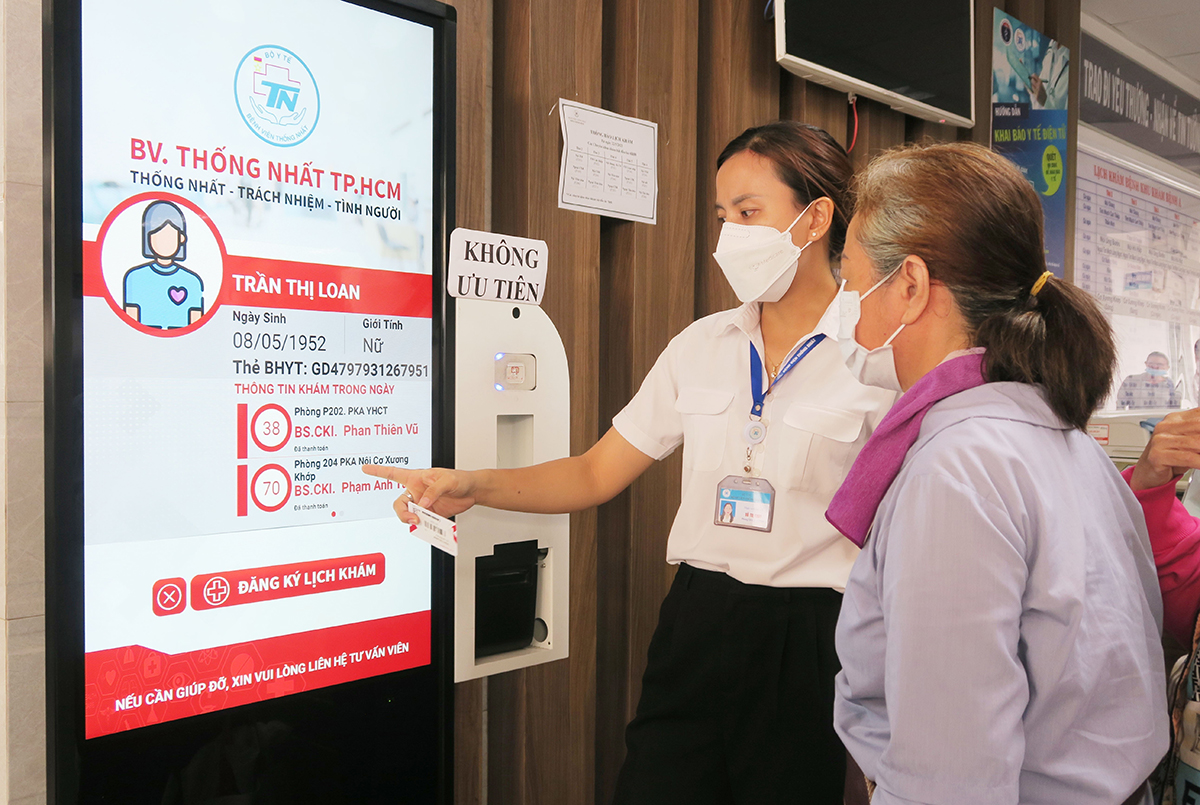
\includegraphics[width=0.5\linewidth]{graphics/ngdan_yte.png}
    \caption{Người bệnh đăng ký khám bệnh tại bảng thông tin điện tử của Bệnh viện Thống Nhất Thành phố Hồ Chí Minh\_Ảnh: TTXVN}
\end{figure}

\textbf{Đối với nhân viên y tế:}

Chuyển đổi số y tế giúp các bác sĩ dễ dàng tiếp cận kiến thức và kỹ thuật y học mới nhất, nâng cao chất lượng và an toàn cho bệnh nhân. Ngoài ra, chuyển đổi số cũng giảm thiểu nguy cơ sai sót trong các quy trình y tế, đảm bảo sự chính xác và đáng tin cậy trong quản lý thông tin y tế. Các công nghệ mới giúp nhân viên y tế cải thiện hiệu suất và chất lượng công việc, đồng thời nâng cao sự hài lòng của bệnh nhân.
Hệ thống quản lý thông tin y tế đã giúp tạo điều kiện thuận lợi cho việc truy cập và chia sẻ thông tin của bệnh nhân giữa các bác sĩ, cơ sở khám chữa bệnh. Điều này cho phép các chuyên gia y tế kết nối và tương tác dễ dàng hơn.

Mục tiêu của việc chuyển đổi số y tế là xây dựng hồ sơ bệnh án điện tử tại mỗi bệnh viện và cơ sở khám chữa bệnh.

Chuyển đổi số trong lĩnh vực y tế mang lại nhiều lợi ích cho việc quản lý sức khỏe và cung cấp dịch vụ chăm sóc. Công nghệ giúp các nhà quản lý y tế hiệu quả hơn trong công tác điều phối, giám sát, cảnh báo và dự báo về các vấn đề sức khỏe của người dân.
Chuyển đổi số đóng vai trò hết sức quan trọng trong tiến trình cải cách thủ tục hành chính của ngành y tế. Bằng việc áp dụng các ứng dụng và hệ thống trực tuyến, ngành y tế có thể giảm thiểu các thủ tục phức tạp, thời gian chờ đợi và cung cấp dịch vụ chăm sóc sức khỏe thuận lợi hơn cho người dân.

Chuyển đổi số cũng giúp tăng cường tính tiếp cận và hiệu quả khi thực hiện các dịch vụ y tế. Từ đó, chất lượng phục vụ cho người bệnh và nhân viên y tế có thể được nâng cao đáng kể.

Các ứng dụng hữu ích của chuyển đổi số cũng mang lại nhiều lợi ích cho nhà quản lý bệnh viện và cơ sở y tế. Các ứng dụng này giúp quản lý quy trình, phác đồ điều trị của nhân viên y tế và triển khai các công việc nhằm nâng cao chất lượng phục vụ cho người bệnh và nhân viên y tế.

\newpage

\begin{figure}[!htp]
    \centering
    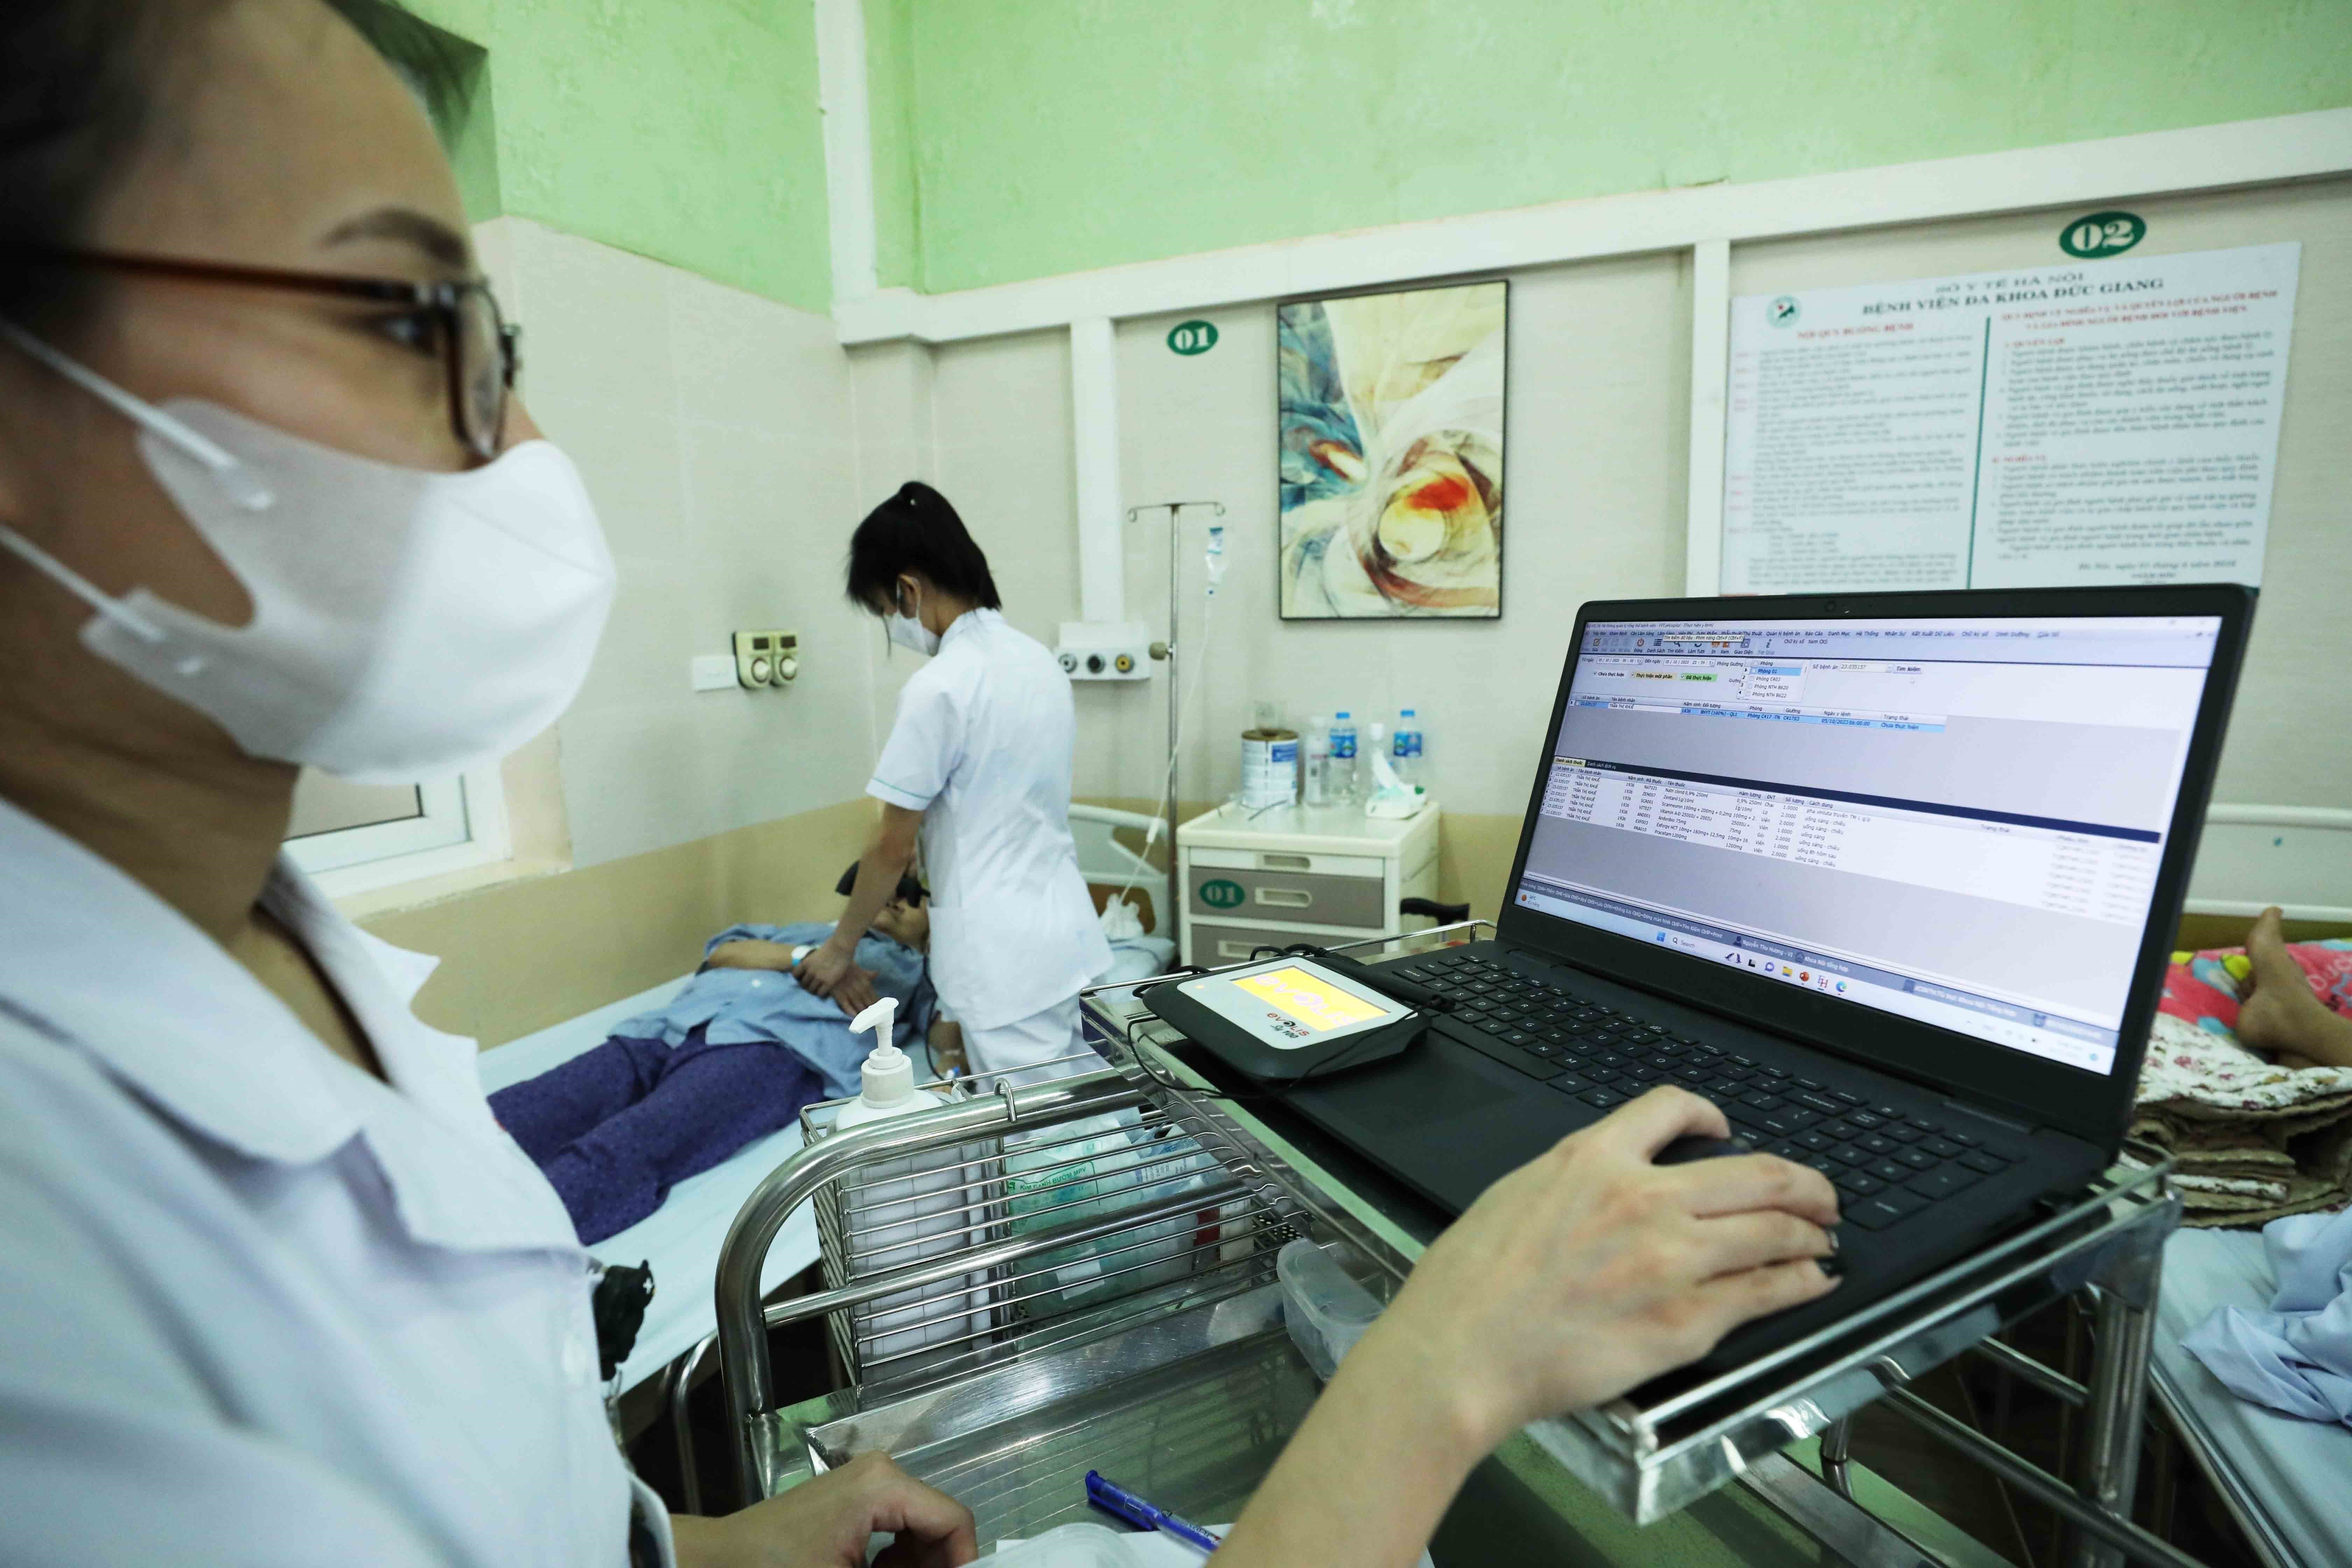
\includegraphics[width=0.6\linewidth]{graphics/bacsi_qr.png}
    \caption{Bệnh viện Đa khoa Đức Giang sử dụng mã QR Code cấp cho bệnh nhân giúp điều dưỡng viên nắm thông tin bệnh nhân thông qua thiết bị quét mã, hiển thị lên màn hình máy tính đặt trên xe thuốc\_Ảnh: TTXVN}
\end{figure}

\subsubsection{Thực trạng chuyển đổi số y tế tại Việt Nam}
Một nghiên cứu gần đây của Trường Đại học Kinh tế Tp. Hồ Chí Minh đã chỉ ra rằng Việt Nam, đặc biệt là TP.HCM, đã tương đối kiểm soát và ổn định được tình hình đại dịch COVID-19 trong vài năm trở lại đây. Dù đã kiểm soát được đại dịch nhưng dấu ấn còn lại của sự tàn phá khủng khiếp vẫn tiếp tục đọng lại trong tâm trí người dân.

Trong bối cảnh ứng dụng Công nghệ thông tin và chuyển đổi số trong công tác phòng chống dịch, Thành phố Hồ Chí Minh đã thể hiện sự sáng tạo và hiệu quả đáng ghi nhận. Một ví dụ điển hình cho điều này là hệ thống quản lý người bệnh COVID-19 được Sở Y tế TP.HCM phát triển và ra mắt vào đầu tháng 3/2022.

Trước đó, hàng nghìn người đến các trung tâm y tế chờ đợi để khai báo đã mắc COVID-19 (F0) và hàng nghìn người khác chờ đợi để nhận giấy xác nhận đã hoàn thành thời gian cách ly tại nhà. Tuy nhiên, nhờ vào hệ thống quản lý này, Thành phố đã giải quyết triệt để tình trạng tắc nghẽn của người bệnh tại các trung tâm y tế trên toàn thành phố.
Việt Nam đang đặt phát triển chăm sóc sức khỏe là một ưu tiên hàng đầu. Chi tiêu cho lĩnh vực y tế đang có sự tăng trưởng mạnh mẽ, từ 15,6 tỷ USD trong năm 2018 lên 42,9 tỷ USD vào năm 2028, tương đương mức tăng trưởng kép hàng năm (CAGR) là 11\% trong 10 năm. Điều này giúp Việt Nam trở thành quốc gia đầu tư nhiều nhất vào lĩnh vực chăm sóc sức khỏe trong khu vực ASEAN. Mức chi tiêu bình quân đầu người cho chăm sóc sức khỏe cũng dự kiến sẽ tăng lên 408 USD/năm vào năm 2028, gấp ba lần so với mức 141 USD/năm năm 2018.

Việt Nam có nhiều điều kiện thuận lợi để áp dụng các giải pháp y tế số. Các công nghệ mới đã nhanh chóng được đón nhận bởi hơn 60\% dân số Việt Nam dưới 54 tuổi. Người dân Việt Nam dành khoảng 7 giờ mỗi ngày cho các hoạt động trực tuyến, và 3 giờ trong số đó được thực hiện trên các thiết bị di động.

Việt Nam đã thực hiện nhiều chính sách để xây dựng cơ sở hạ tầng và phát triển các dịch vụ công nghệ thông tin và truyền thông. Việc truy cập internet đã được lan rộng trên toàn quốc, với tỷ lệ sử dụng đạt 67\% vào năm 2017, và tốc độ tăng trưởng hàng năm của việc sử dụng internet là 28\%. Công nghệ thông tin di động cũng đang phát triển mạnh mẽ tại Việt Nam, với mạng 4G đã có phủ sóng đến hơn 95\% các hộ gia đình.

Việc áp dụng các giải pháp y tế số tại Việt Nam sẽ mang lại nhiều lợi ích. Điều này bao gồm khả năng truy cập thông tin y tế và dịch vụ y tế từ xa, cũng như khả năng theo dõi và quản lý sức khỏe của người dân một cách hiệu quả hơn.

Cơ sở hạ tầng công nghệ ở Việt Nam đang hướng tới việc ứng dụng các dịch vụ dựa trên nền tảng lưu trữ đám mây, tạo điều kiện thuận lợi cho việc triển khai các giải pháp sáng tạo và hiệu quả về chi phí trong lĩnh vực chăm sóc sức khỏe.

Bộ Y tế đã đưa ra một kế hoạch để triển khai ứng dụng công nghệ thông tin và chuyển đổi số tại các cơ sở khám chữa bệnh. Theo đó, các bệnh viện sẽ phải thực hiện chuyển đổi số trước ngày 1/1/2027 để được cấp giấy phép hoạt động kể từ năm nay.

Các bệnh viện được cấp giấy phép hoạt động trước ngày 1/1/2027 sẽ có thời gian đến ngày 1/1/2029 để hoàn thành chuyển đổi số.

\begin{figure}[!htp]
    \centering
    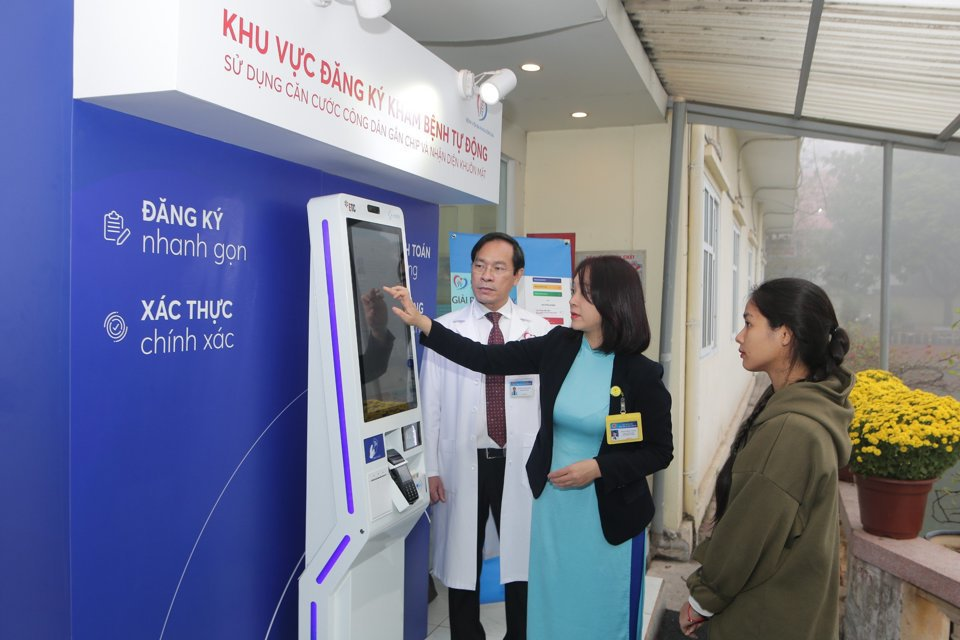
\includegraphics[width=0.6\linewidth]{graphics/faceid.png}
    \caption{Bệnh viện Đa khoa Đống Đa đã lắp đặt tại sảnh khoa Khám bệnh một máy đăng ký khám bệnh và phát số tự động sử dụng CCCD gắn chíp và nhận diện khuôn mặt.}
\end{figure}

\subsection{Thiết bị cân điện tử thông minh và tiềm năng ứng dụng}

Thị trường cân sức khỏe thông minh hiện nay đang ngày càng đa dạng với nhiều lựa chọn hấp dẫn như \textbf{Xiaomi Smart Scale 2} và \textbf{CRENOT Gofit S2}. Cả hai thiết bị này đều được trang bị công nghệ hiện đại, giúp người dùng theo dõi sức khỏe một cách chính xác và tiện lợi.

\textbf{Xiaomi Smart Scale 2} nổi bật với thiết kế đơn giản, hiện đại và khả năng kết nối nhanh chóng với ứng dụng Mi Fit. Thiết bị này cho phép người dùng đo được nhiều chỉ số cơ thể quan trọng như cân nặng, chỉ số khối cơ thể (BMI), tỷ lệ mỡ trong cơ thể, lượng nước trong cơ thể và khối lượng xương. Bên cạnh đó, Xiaomi Smart Scale 2 còn có khả năng nhận diện tới 16 người dùng khác nhau, rất phù hợp với những gia đình đông thành viên.

\begin{figure}[!htp]
    \centering
    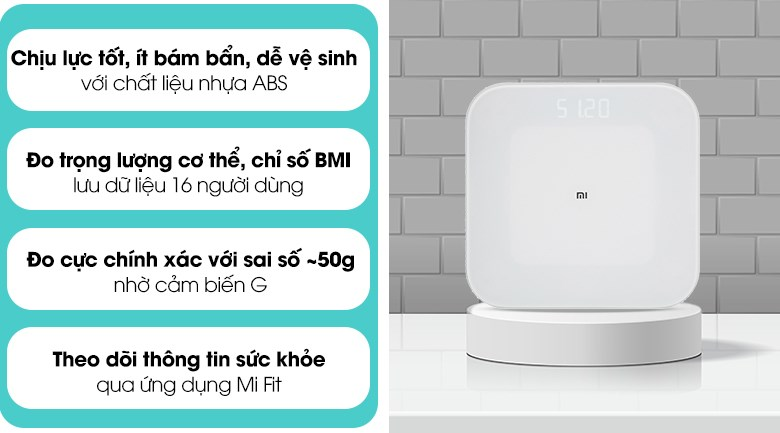
\includegraphics[width=0.8\linewidth]{graphics/xiaomi_scale2.jpg}
    \caption{Thông tin chi tiết của sản phẩm Xiaomi Smart Scale 2}
\end{figure}

Trong khi đó, \textbf{CRENOT Gofit S2} lại gây ấn tượng với độ chính xác cao nhờ sử dụng công nghệ phân tích trở kháng điện sinh học (BIA) kết hợp với chip cảm biến ZeroVar. Thiết bị này cung cấp một danh sách dài các chỉ số sức khỏe chi tiết hơn, giúp người dùng có cái nhìn toàn diện về tình trạng cơ thể của mình. Ngoài ra, CRENOT Gofit S2 còn có khả năng đồng bộ dữ liệu với nhiều ứng dụng sức khỏe khác nhau, tạo điều kiện cho người dùng quản lý thông tin một cách linh hoạt.

\newpage

\begin{figure}[!htp]
    \centering
    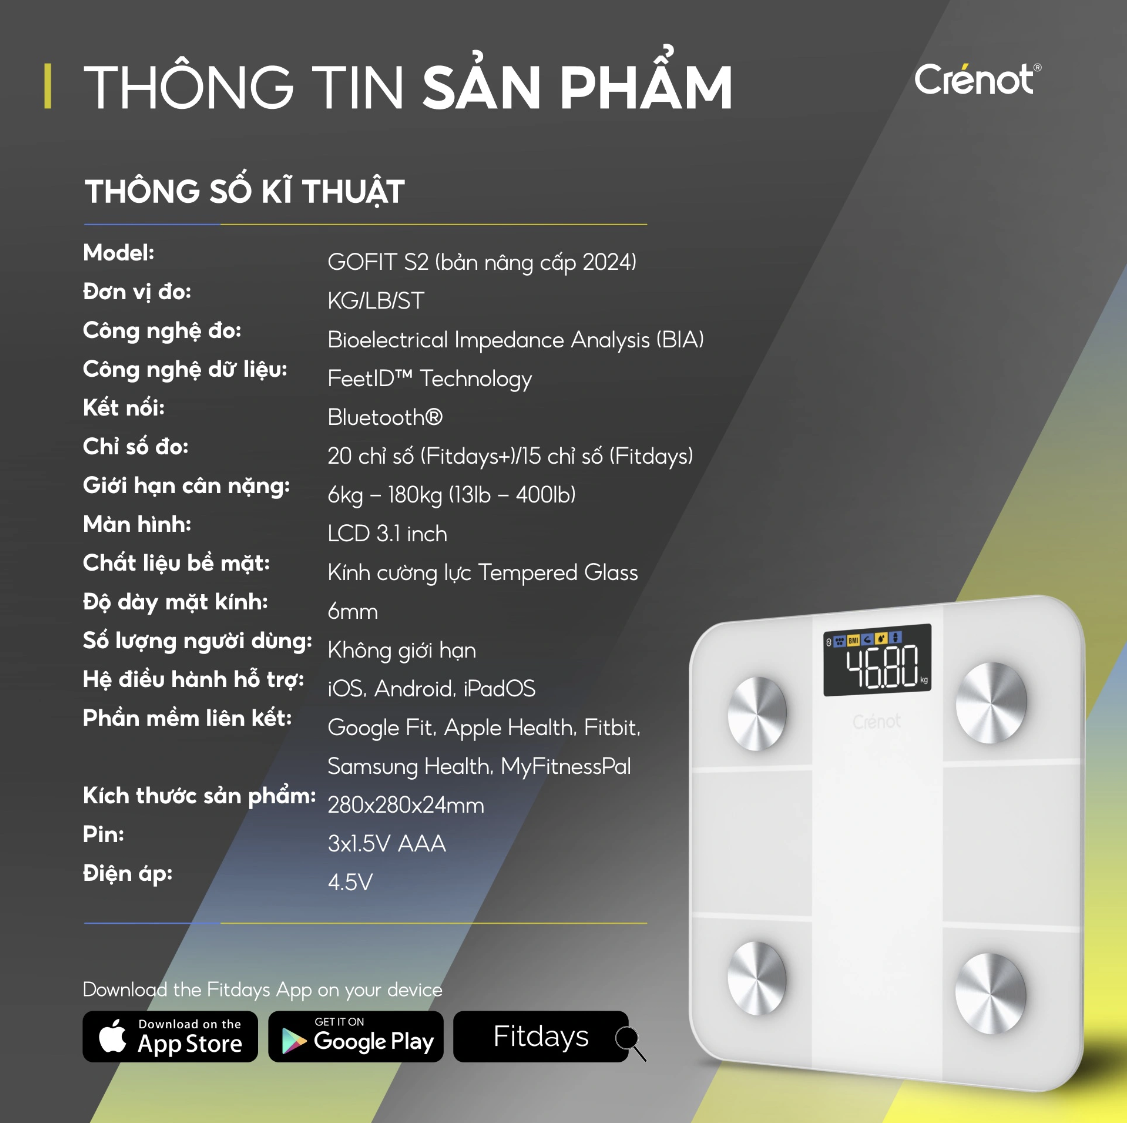
\includegraphics[width=0.7\linewidth]{graphics/info_crenot.png}
    \caption{Thông tin chi tiết của sản phẩm CRENOT Gofit S2}
\end{figure}

Xây dựng hệ thống chăm sóc sức khỏe điện tử với thiết bị cân điện tử sức khoẻ thông minh không chỉ mang lại những lợi ích cho cá nhân người sử dụng, mà còn đóng góp vào quá trình quản lý sức khỏe cộng đồng tại Việt Nam. Hệ thống này sẽ tận dụng dữ liệu được thu thập từ các thiết bị để cung cấp thông tin tổng quan về sức khỏe, giúp người dùng để phát hiện sớm những thay đổi tiêu cực trong cơ thể và có các biện pháp can thiệp kịp thời. 

Ngoài ra, hệ thống còn có thể tích hợp với các nền tảng khác như điện thoại thông minh, máy tính bảng và máy tính cá nhân thông qua các ứng dụng y tế hoặc nền tảng quản lý sức khỏe từ xa. Dữ liệu từ thiết bị cân thông minh được truyền qua kết nối Bluetooth hoặc Wi-Fi đến các ứng dụng quản lý sức khỏe, từ đó được lưu trữ trên hệ thống đám mây. Nhờ vào việc sử dụng trí tuệ nhân tạo (AI) và các công cụ phân tích dữ liệu lớn (Big Data), hệ thống có khả năng phân tích, đưa ra các gợi ý về sức khỏe, từ khuyến nghị về chế độ ăn uống, tập luyện cho đến các cảnh báo về nguy cơ bệnh tật.

Với xu hướng chuyển đổi số tại Việt Nam, hệ thống này còn có tiềm năng tích hợp với các hệ thống quản lý y tế cộng đồng, giúp các cơ sở y tế và bệnh viện dễ dàng theo dõi sức khỏe từ xa của bệnh nhân, đặc biệt là các bệnh nhân mắc bệnh mãn tính như tiểu đường, huyết áp cao hay béo phì. Điều này sẽ giảm tải áp lực cho hệ thống y tế, đặc biệt trong bối cảnh bệnh viện và các cơ sở y tế đang quá tải do số lượng bệnh nhân lớn.

\subsection{Các hệ thống tham chiếu trong nghiên cứu}
\subsubsection{Cân thông minh Xiaomi Body Scale S400 \cite{s400:online}}
Xiaomi Body Scale S400 là sản phẩm được người tiêu dùng sử dụng rộng rãi và vô cùng phổ biến ở thị trường trong và ngoài nước cũng là một trong những thiết bị thông minh đáng chú ý trong hệ sinh thái Xiaomi, được thiết kế để trở thành thiết bị chăm sóc sức khoẻ đáng tin cậy cho mỗi thành viên trong gia đình. Với thiết kế hiện đại và khả năng đo lường chính xác, sản phẩm này mang đến cho người dùng cái nhìn sâu sắc về tình trạng sức khỏe của bản thân, từ đó hỗ trợ xây dựng một lối sống lành mạnh và bền vững.

\begin{figure}[!htp]
    \centering
    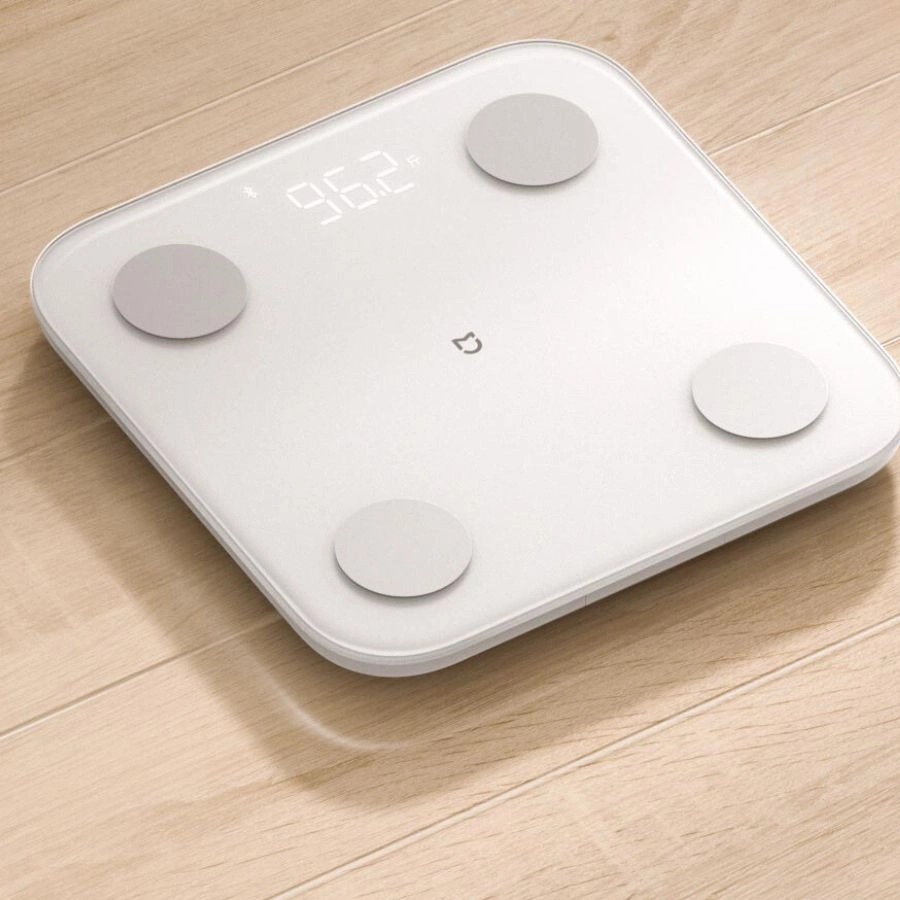
\includegraphics[width=0.6\linewidth]{graphics/s400.png}
    \caption{Cân Thông Minh Xiaomi Body Scale S400}
\end{figure}

Không chỉ đơn thuần là một chiếc cân, Xiaomi Body Scale S400 còn là một công cụ phân tích cơ thể toàn diện. Thiết bị này cung cấp hơn 10 chỉ số sức khỏe quan trọng, bao gồm một số tính năng nổi bật như:

\begin{itemize}
    \item \textbf{Cân nặng:} Theo dõi sự thay đổi cân nặng theo thời gian để đánh giá hiệu quả của quá trình giảm cân hoặc tăng cân.
    \item \textbf{Chỉ số khối cơ thể (BMI):} Đánh giá tình trạng cân nặng có phù hợp với chiều cao hay không, từ đó xác định nguy cơ mắc các bệnh liên quan đến béo phì hoặc suy dinh dưỡng.
    \item \textbf{Tỷ lệ mỡ cơ thể:} Cho biết lượng mỡ trong cơ thể, giúp bạn điều chỉnh chế độ ăn uống và tập luyện để đạt được tỷ lệ mỡ lý tưởng.
    \item \textbf{Tỷ lệ cơ bắp:} Đánh giá khối lượng cơ, giúp bạn theo dõi sự phát triển cơ bắp và xây dựng cơ thể săn chắc.
    \item \textbf{Khối lượng xương:} Giúp bạn theo dõi sức khỏe xương và phòng ngừa các bệnh về xương khớp.
    \item \textbf{Tỷ lệ nước trong cơ thể:} Cho biết lượng nước trong cơ thể, giúp bạn điều chỉnh lượng nước uống hàng ngày để duy trì sự cân bằng điện giải.
    \item Và nhiều chỉ số khác: Như khối lượng nội tạng, tuổi cơ thể, v.v., giúp bạn hiểu rõ hơn về tình trạng sức khỏe của mình.
\end{itemize}

\begin{figure}[!htp]
    \centering
    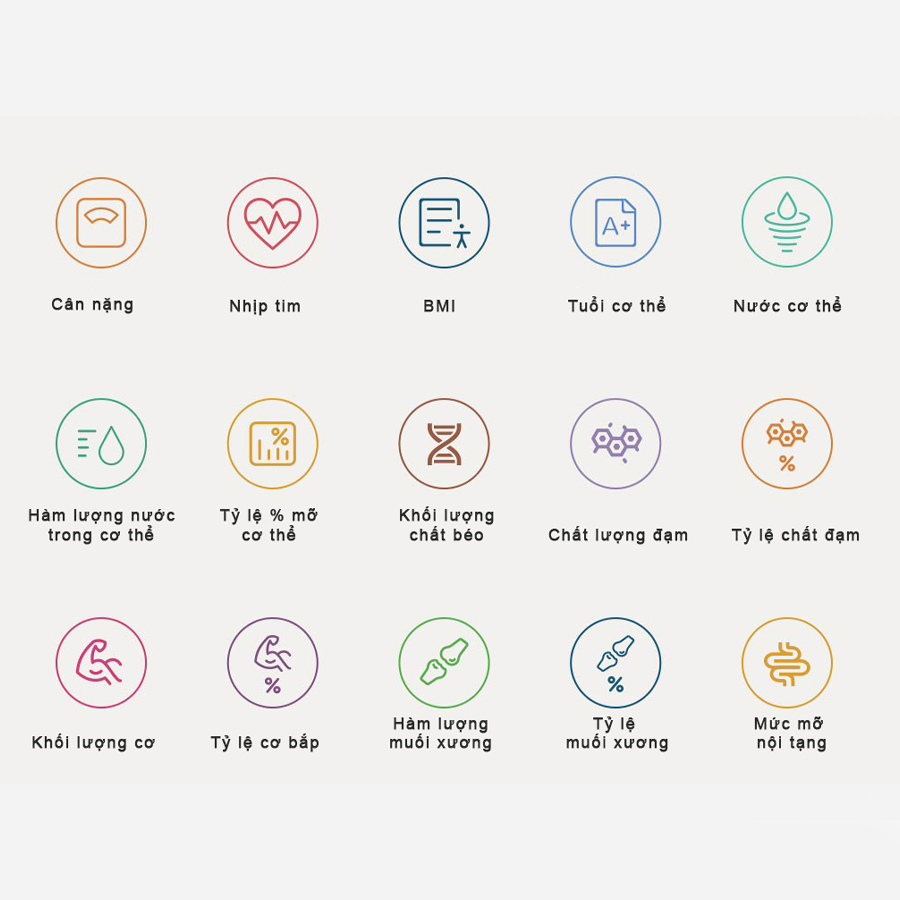
\includegraphics[width=0.6\linewidth]{graphics/thong_so_sk.png}
    \caption{Sự đa dạng về các chỉ số sức khoẻ mà S400 có thể đo được}
\end{figure}

Cân thông minh Xiaomi Body Scale S400 có thể kết nối với ứng dụng Mi Fit hoặc Zepp Life thông qua Bluetooth. Nhờ đó, người dùng có thể:

\begin{itemize}
    \item \textbf{Theo dõi dữ liệu theo thời gian thực:} Quan sát sự thay đổi của các chỉ số sức khỏe qua từng ngày, tuần hoặc tháng.
    \item \textbf{Trực quan hóa kết quả:} Biểu đồ và đồ thị trực quan giúp bạn dễ dàng nắm bắt tình hình sức khỏe của mình.
    \item \textbf{Nhận khuyến nghị cá nhân hóa:} Ứng dụng sẽ đưa ra các gợi ý về chế độ ăn uống và tập luyện phù hợp với mục tiêu của bạn.
    \item \textbf{Chia sẻ dữ liệu với chuyên gia:} Bạn có thể chia sẻ dữ liệu với bác sĩ hoặc chuyên gia dinh dưỡng để được tư vấn cụ thể hơn.
\end{itemize}

\begin{figure}[!htp]
    \centering
    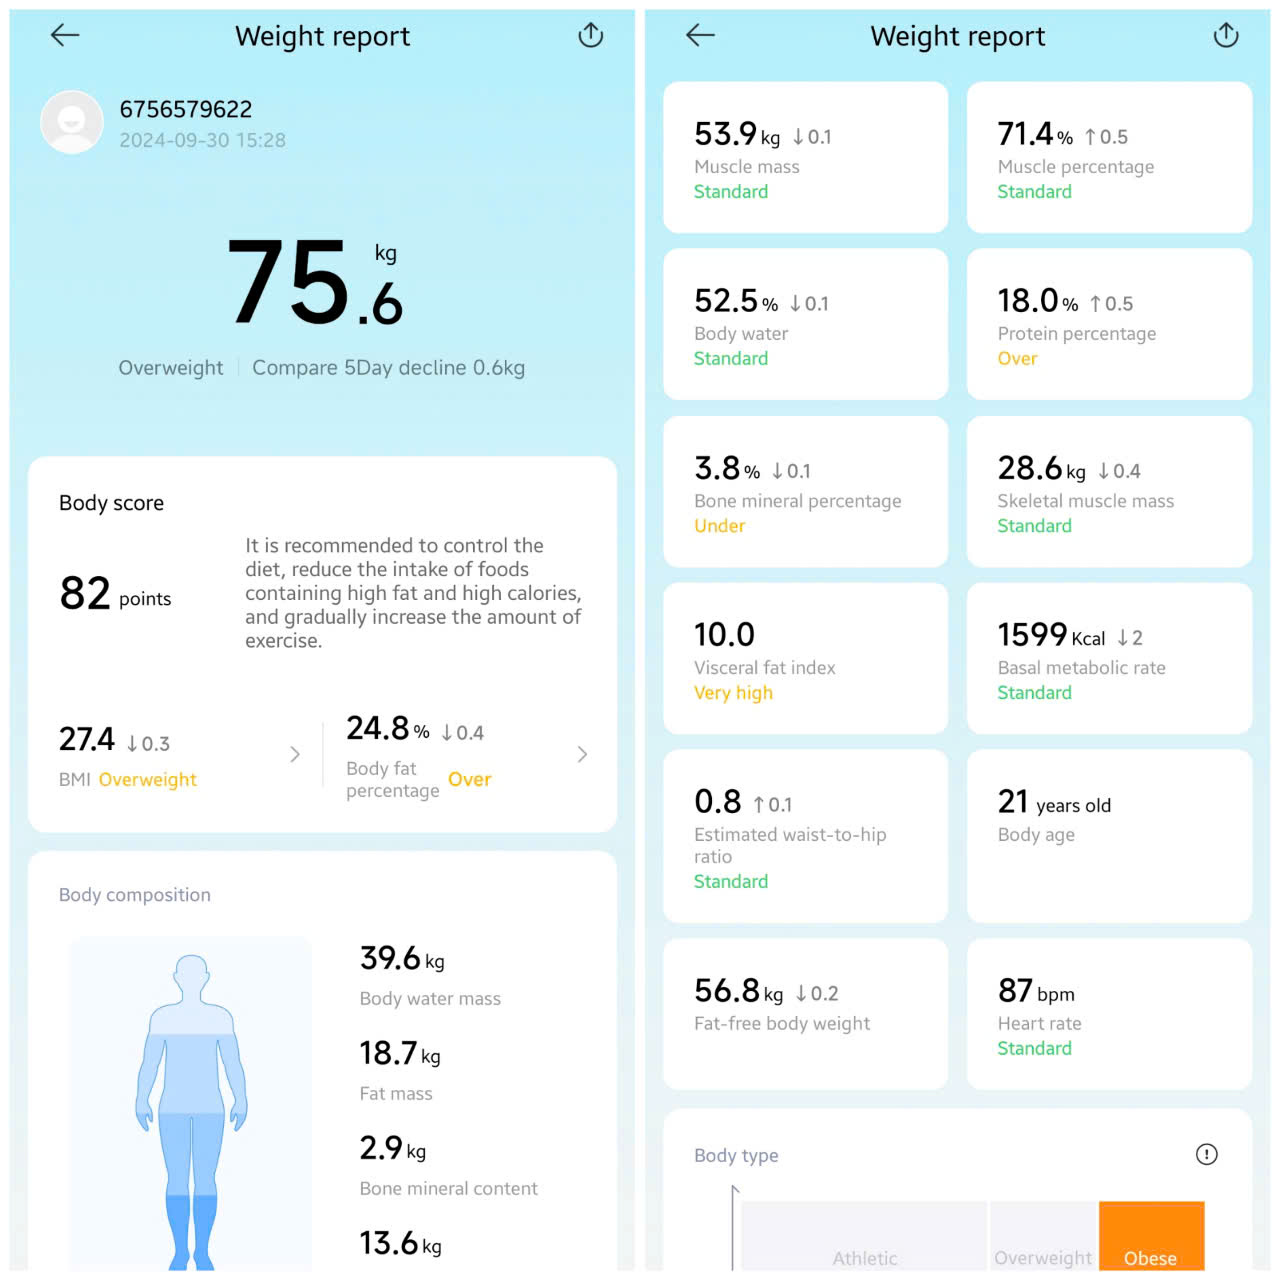
\includegraphics[width=0.5\linewidth]{graphics/info_user.png}
    \caption{Các chỉ số sức khoẻ của người dùng được thể hiện và đồng bộ hoá trên ứng dụng Mi Home}
\end{figure}

Xiaomi Body Scale S400 là một phần không thể thiếu trong hệ sinh thái nhà thông minh của Xiaomi. Người dùng có thể kết nối cân với các thiết bị khác như đồng hồ thông minh, điện thoại di động để tạo ra một hệ thống quản lý sức khỏe toàn diện.

\textbf{Ưu điểm nổi bật:}
\begin{itemize}
    \item \textbf{Thiết kế hiện đại, sang trọng:} Phù hợp với mọi không gian sống.
    \item \textbf{Dễ sử dụng:} Chỉ cần đứng lên cân là có thể đo được các chỉ số.
    \item \textbf{Độ chính xác cao:} Đảm bảo kết quả đo lường đáng tin cậy.
    \item \textbf{Tính năng nhận diện nhiều người dùng:} Phù hợp cho cả gia đình.
    \item \textbf{Giá cả phải chăng:} So với các sản phẩm cùng loại trên thị trường.
\end{itemize}

\textbf{Hạn chế:}
\begin{itemize}
    \item \textbf{Phụ thuộc vào kết nối Bluetooth:} Nếu kết nối không ổn định có thể ảnh hưởng đến việc đồng bộ dữ liệu.
    \item \textbf{Không hỗ trợ đồng bộ trực tiếp với một số ứng dụng sức khỏe khác:} Bạn có thể cần sử dụng các ứng dụng chuyển đổi dữ liệu.
\end{itemize}

\subsubsection{Cân thông minh 365 Selection WS1 \cite{ws1:online}}
Với một mặt kính cường lực trong suốt, cân sức khoẻ 365 Selection WS1 của Thái Lan có kiểu dáng sang trọng, tinh tế và đẹp mắt. Cân đo 18 chỉ số cơ thể, kết nối Bluetooth với điện thoại di động thông qua ứng dụng 365 Life và tự động nhận dạng người dùng. Màn hình LED hiển thị rõ ràng và chi tiết. Đây là lựa chọn hoàn hảo thiết bị chăm sóc và theo dõi sức khoẻ của mỗi gia đình.

\begin{figure}[!htp]
    \centering
    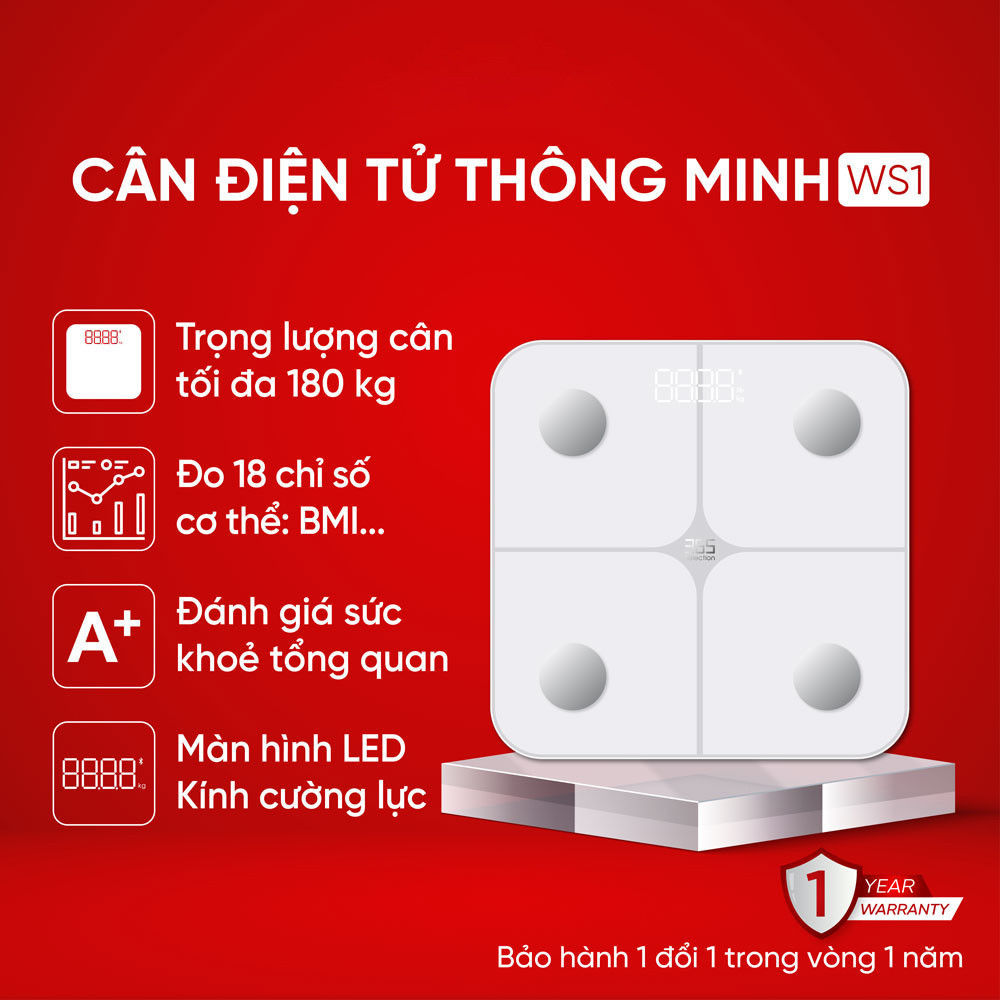
\includegraphics[width=0.6\linewidth]{graphics/ws1.png}
    \caption{Cân thông minh 365 Selection WS1}
\end{figure}

Được trang bị cảm biến chất lượng cao, cân thông minh 365 Selection WS1 đảm bảo đo lường trọng lượng với độ chính xác cao cùng tốc độ nhanh. Các cảm biến này cung cấp những thông số trọng lượng vô cùng chính xác và đáng tin cậy, cho phép người dùng đo lường và theo dõi trọng lượng cơ thể dễ dàng.

\begin{figure}[!htp]
    \centering
    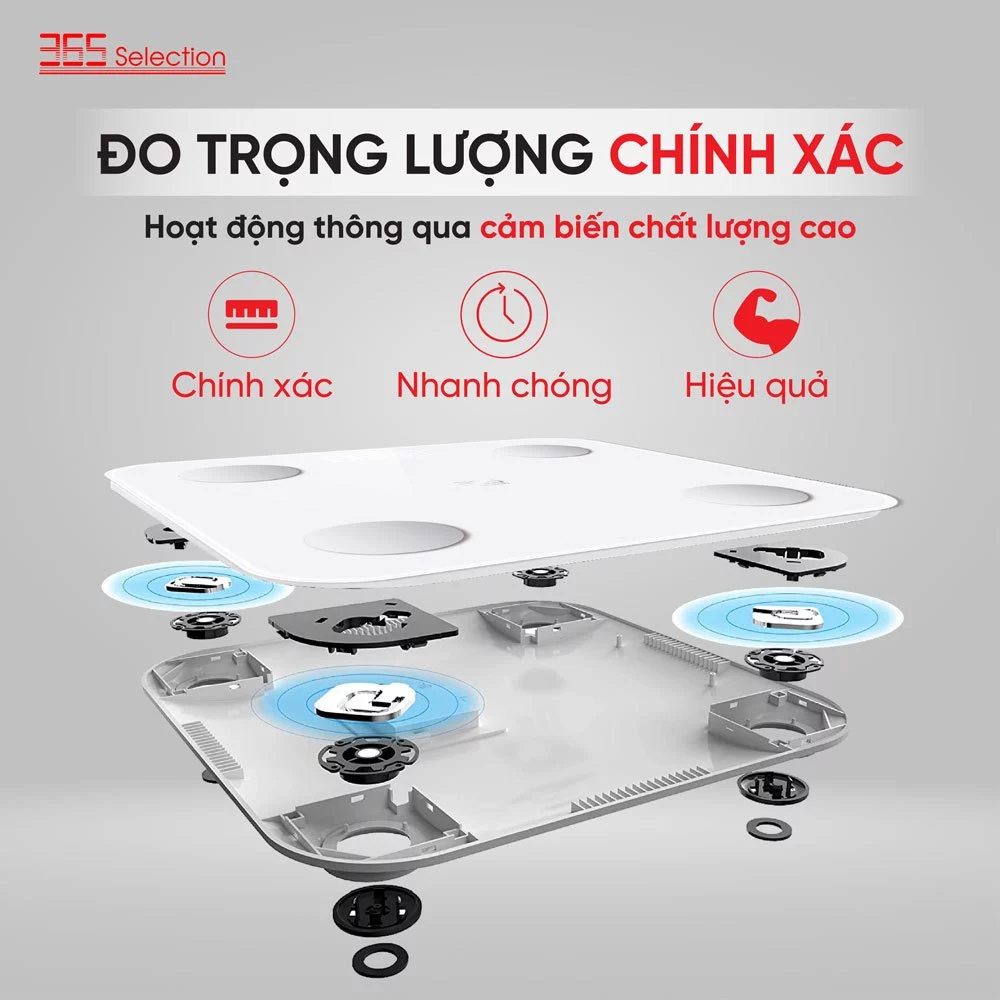
\includegraphics[width=0.6\linewidth]{graphics/sensors.png}
    \caption{Cảm biến chất lượng cao của WS1}
\end{figure}

Không chỉ đo trọng lượng chuẩn xác mà cân thông minh 365 Selection WS1 còn phân tích 18 chỉ số sức khoẻ quan trọng.

\begin{itemize}
    \item \textbf{Cân nặng:} Đo trọng lượng cơ thể tổng quát.
    \item BMI (Chỉ số khối cơ thể): Đánh giá sự cân đối giữa trọng lượng và chiều cao, giúp xác định mức độ béo phì hoặc thiếu cân.
    \item \textbf{Tỷ lệ mỡ cơ thể:} Xác định phần trăm mỡ so với tổng trọng lượng cơ thể, phản ánh mức độ mỡ cơ thể tổng quát.
    \item \textbf{Khối lượng cơ:} Đo lượng cơ bắp trong cơ thể, hữu ích để theo dõi sự phát triển cơ bắp và sức mạnh.
    \item \textbf{Khối lượng mỡ:} Đo lượng mỡ cơ thể toàn thân, giúp xác định mức độ mỡ dư thừa.
    \item \textbf{Chỉ số mỡ cơ thể:} Đánh giá mức độ phân bổ mỡ trong cơ thể, cung cấp cái nhìn về sự phân bố mỡ giữa các vùng cơ thể.
    \item \textbf{Mức độ béo phì:} Phân loại mức độ béo phì dựa trên tỷ lệ mỡ cơ thể và BMI, giúp xác định nguy cơ sức khỏe liên quan đến béo phì.
    \item \textbf{Cân nặng lý tưởng:} Cung cấp trọng lượng cơ thể lý tưởng dựa trên các yếu tố như chiều cao, tuổi, và giới tính.
    \item \textbf{Kiểm soát cân nặng:} Theo dõi sự thay đổi cân nặng theo thời gian để giúp bạn duy trì hoặc điều chỉnh mục tiêu cân nặng.
    \item \textbf{Chỉ số mỡ nội tạng:} Đo lượng mỡ xung quanh các cơ quan nội tạng, giúp đánh giá nguy cơ mắc bệnh tim mạch và các vấn đề sức khỏe khác.
    \item \textbf{Cân nặng trừ mỡ:} Xác định trọng lượng cơ thể sau khi trừ đi lượng mỡ, giúp phân tích khối lượng cơ và xương.
    \item \textbf{Nước trong cơ thể:} Đo lượng nước chiếm tỷ lệ trong cơ thể, phản ánh tình trạng hydrat hóa và sức khỏe tổng quát.
    \item \textbf{Khối lượng xương:} Đo lượng xương trong cơ thể, giúp theo dõi sức khỏe xương và nguy cơ loãng xương.
    \item \textbf{Tỷ lệ Protein:} Xác định tỷ lệ protein trong cơ thể, phản ánh tình trạng dinh dưỡng và sức khỏe cơ bắp.
    \item \textbf{BMR (Tỷ lệ trao đổi chất cơ bản):} Đánh giá số lượng calo cơ thể cần tiêu thụ để duy trì các chức năng cơ bản khi nghỉ ngơi.
    \item \textbf{Tuổi chuyển hóa:} Đo lường sự chuyển hóa cơ thể so với tuổi thực tế, giúp đánh giá tốc độ trao đổi chất và sức khỏe tổng quát.
    \item \textbf{Phân loại sức khỏe:} Xếp loại sức khỏe tổng thể dựa trên các chỉ số đo được, giúp bạn dễ dàng đánh giá tình trạng cơ thể.
    \item \textbf{Điểm số cơ thể:} Cung cấp một điểm số tổng hợp phản ánh tình trạng sức khỏe tổng thể, hỗ trợ bạn trong việc theo dõi và cải thiện lối sống.
\end{itemize}

Cân thông minh 365 Selection WS1 cho phép lưu trữ và cập nhật dữ liệu sức khoẻ trên ứng dụng 365 Life thông qua kết nối bluetooth. Cho phép người dùng nhanh chóng nắm bắt và theo dõi được tình trạng sức khoẻ qua từng lượt đo, có cái nhìn tổng quan về mức độ phát triển và tình trạng sức khoẻ của người dùng.

\newpage

\begin{figure}[!htp]
    \centering
    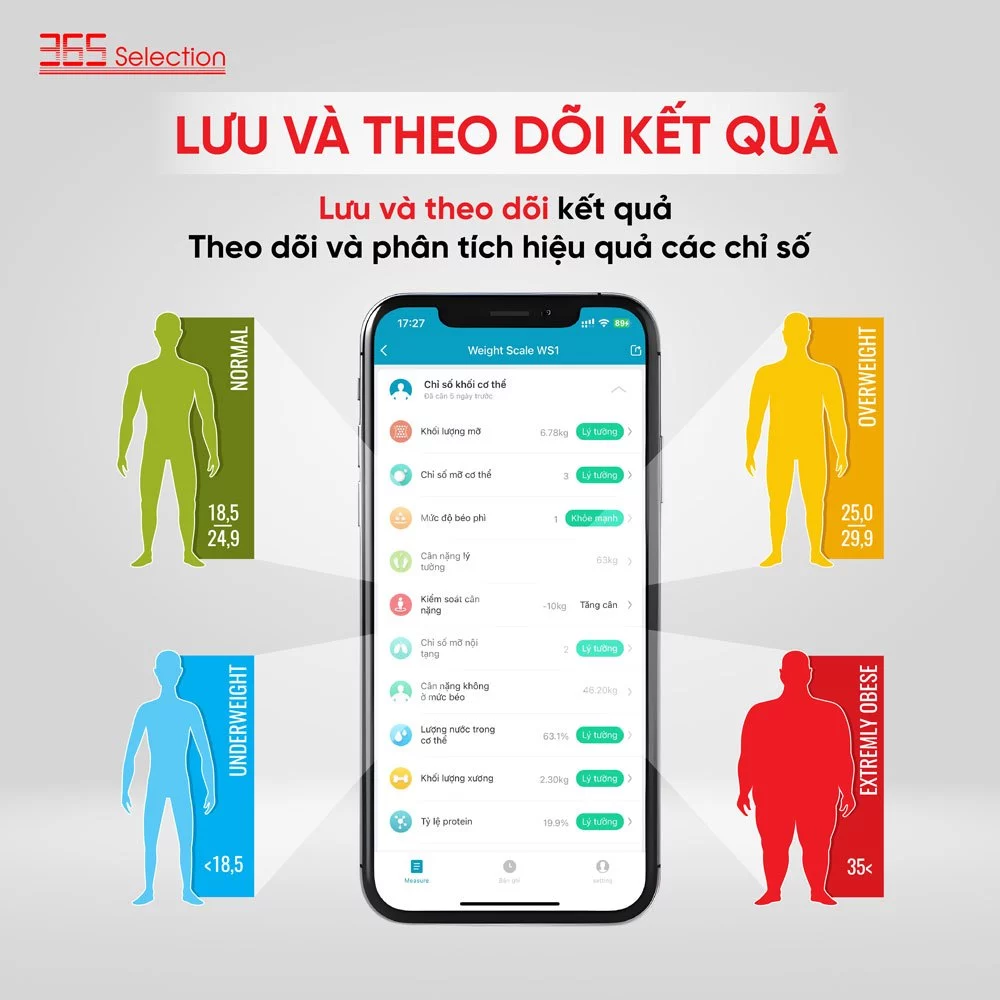
\includegraphics[width=0.6\linewidth]{graphics/theodoichiso.png}
    \caption{Khả năng lưu trữ và cập nhật dữ liệu}
\end{figure}

Ngoài ra, sản phẩm còn hỗ trợ lưu trữ kết quả đo cho tối đa 10 người, cân thông minh sẽ cho phép tất cả gia đình cùng sử dụng. Cân sẽ tự động nhận diện người sử dụng dựa trên các dữ liệu trước đó hoặc nhận diện người mới khi các chỉ số được đo. Trong ứng dụng 365 Life, kết quả đo sẽ được lưu trữ tự động, giúp bạn giám sát và theo dõi tình hình sức khoẻ của các thành viên trong gia đình một cách thuận tiện và dễ dàng.

\subsection{Thách thức và cơ hội triển khai tại Việt Nam}

Việt Nam đang trong giai đoạn thúc đẩy mạnh mẽ quá trình chuyển đổi số trong nhiều lĩnh vực, bao gồm cả y tế. Các cơ hội để phát triển và triển khai hệ thống chăm sóc sức khỏe điện tử rất lớn, nhờ vào sự hỗ trợ từ chính sách của chính phủ và tốc độ phát triển công nghệ. Cùng với sự phát triển của hạ tầng viễn thông và Internet, người dân Việt Nam ngày càng có khả năng tiếp cận các dịch vụ y tế thông minh, từ đó giúp nâng cao ý thức về chăm sóc sức khỏe.

Tuy nhiên, việc triển khai hệ thống chăm sóc sức khỏe điện tử tại Việt Nam vẫn đối mặt với một số thách thức. Đầu tiên là vấn đề về hạ tầng công nghệ, đặc biệt ở các khu vực nông thôn và vùng sâu, vùng xa. Khả năng tiếp cận Internet và các thiết bị thông minh ở những khu vực này còn hạn chế, do đó việc triển khai hệ thống có thể gặp khó khăn trong việc tiếp cận người dùng. Thứ hai, là vấn đề bảo mật và quyền riêng tư của dữ liệu sức khỏe cá nhân. Khi dữ liệu sức khỏe được thu thập và lưu trữ trên các hệ thống đám mây, cần có các biện pháp bảo mật chặt chẽ để đảm bảo không xảy ra các sự cố lộ lọt thông tin cá nhân.

\subsection{Tầm quan trọng của hệ thống trong tương lai}

Việc xây dựng một hệ thống chăm sóc sức khỏe điện tử với thiết bị CRENOT Gofit S2 phù hợp với xu hướng toàn cầu về chăm sóc sức khỏe thông minh, đồng thời góp phần vào việc cải thiện chất lượng chăm sóc sức khỏe tại Việt Nam. Hệ thống không chỉ đáp ứng nhu cầu của cá nhân trong việc theo dõi sức khỏe mà còn cung cấp một công cụ hỗ trợ đắc lực cho các cơ sở y tế trong quản lý sức khỏe cộng đồng, giảm tải gánh nặng cho hệ thống y tế hiện tại.

Với sự phát triển của trí tuệ nhân tạo và phân tích dữ liệu lớn, tương lai của hệ thống chăm sóc sức khỏe điện tử sẽ càng trở nên thông minh và hiệu quả hơn. Các công nghệ này sẽ giúp cá nhân hóa các giải pháp chăm sóc sức khỏe, từ đó không chỉ tăng cường chất lượng cuộc sống của người dân mà còn góp phần vào sự phát triển bền vững của hệ thống y tế Việt Nam.
\section{YÊU CẦU VÀ MỤC TIÊU ĐỀ TÀI}
\subsection{Yêu cầu đề tài}
Đề tài yêu cầu nghiên cứu và triển khai một hệ thống chăm sóc sức khỏe điện tử tích hợp với thiết bị cân thông minh như \textbf{Xiaomi Smart Scale 2} và \textbf{CRENOT Gofit S2}. Thiết bị này sẽ cung cấp các chỉ số sức khỏe cơ bản như cân nặng, tỷ lệ mỡ cơ thể, khối lượng cơ, nước, và xương thông qua công nghệ phân tích trở kháng điện sinh học (BIA). Hệ thống cần đảm bảo các yêu cầu sau:

\begin{enumerate}
    \item \textbf{Thu thập và quản lý dữ liệu tự động:} Hệ thống phải đảm bảo khả năng thu thập dữ liệu từ thiết bị cân sức khoẻ thông minh và lưu trữ chúng trong 1 file csv với theo từng cá nhân riêng biệt.
    \item \textbf{Vẽ biểu đồ, trực quan hoá dữ liệu:} Dữ liệu được thu thập sẽ được lưu lại trong 1 file csv với mục đích dùng để vẽ các biểu đồ về thông số sức khoẻ qua các ngày khác nhau, với mục đích để tiện cho việc theo dõi của người dùng
    \item \textbf{Phân tích dữ liệu và đưa ra khuyến nghị:} Dựa trên các dữ liệu thu thập, hệ thống cần có khả năng phân tích, đưa ra các khuyến nghị về chế độ dinh dưỡng, tập luyện, và cảnh báo sớm về các vấn đề sức khỏe cho người dùng.
    \item \textbf{Bảo mật và bảo vệ dữ liệu cá nhân:} Hệ thống cần tuân thủ các tiêu chuẩn bảo mật quốc tế về bảo vệ thông tin cá nhân, đảm bảo an toàn cho dữ liệu sức khỏe của người dùng trong quá trình truyền tải và lưu trữ.
\end{enumerate}

\subsection{Mục tiêu đề tài}
Mục tiêu của đề tài là xây dựng một hệ thống chăm sóc sức khỏe điện tử thông minh, giúp người dùng theo dõi và quản lý sức khỏe cá nhân một cách hiệu quả và tiện lợi. Cụ thể:

\begin{enumerate}
    \item \textbf{Tạo nền tảng quản lý sức khỏe toàn diện:} Hệ thống giúp người dùng theo dõi các chỉ số sức khỏe quan trọng từ thiết bị cân sức khoẻ thông minh, đồng thời cung cấp phân tích chi tiết về tình trạng sức khỏe của họ.
    \item \textbf{Cải thiện chất lượng cuộc sống:} Thông qua việc cung cấp thông tin và khuyến nghị sức khỏe, hệ thống sẽ giúp người dùng duy trì lối sống lành mạnh và ngăn ngừa các bệnh liên quan đến cân nặng, chế độ ăn uống và tập luyện không hợp lý.
    \item \textbf{Phát triển giải pháp y tế số:} Đề tài sẽ đóng góp vào sự phát triển của các giải pháp y tế số tại Việt Nam, giúp các cơ sở y tế và bệnh viện quản lý sức khỏe từ xa cho bệnh nhân một cách hiệu quả hơn, đặc biệt trong các trường hợp bệnh mãn tính.
    \item \textbf{Tăng cường nhận thức về chăm sóc sức khỏe:} Hệ thống sẽ giúp nâng cao nhận thức về việc theo dõi và duy trì sức khỏe hàng ngày của cá nhân, khuyến khích họ thường xuyên kiểm tra các chỉ số quan trọng để phát hiện sớm các dấu hiệu bất thường.
\end{enumerate}

Source code của bài báo cáo sẽ được lưu trữ và cập nhật tại đây: \href{https://github.com/DatTwenty3/xiaomi_smart_scale_2}{DatTwenty3 - GitHub}
\section{CƠ SỞ LÝ THUYẾT}
\subsection{Giới thiệu công nghệ Bluetooth Low Energy \cite{BLE:online}}

Thứ nhất, cần làm rõ rằng BLE không thể được coi là phương thức truyền thông duy nhất, vì nó không thay thế hoàn toàn các giao thức không dây khác như Wifi, Zigbee hay ngay cả Bluetooth Classic (phiên bản 2.0). BLE có mục tiêu thiết kế đặc thù hơn, nhắm đến lĩnh vực ứng dụng nhất định.

BLE (Bluetooth phiên bản 4.0 trở lên) được phát triển với những đặc điểm riêng cho các ứng dụng sau đây:

\begin{itemize}
    \item Tiết kiệm năng lượng tối đa, giúp thiết bị có thể hoạt động từ vài tháng đến vài năm chỉ với một viên pin nhỏ như pin đồng xu.
    \item Khoảng cách kết nối ngắn, thường hoạt động hiệu quả trong phạm vi khoảng 10 mét.
    \item Dữ liệu truyền tải ở mức độ thấp, rất phù hợp cho các ứng dụng cần điều khiển không liên tục và cảm biến.
\end{itemize}
Một số ứng dụng tiêu biểu của BLE bao gồm thiết bị giám sát sức khỏe, beacon, nhà thông minh, hệ thống an ninh, giải trí, cảm biến gần gũi và trong ngành công nghiệp ô tô. Trung tâm của nhiều hệ thống sử dụng BLE thường là smartphone, máy tính bảng và máy tính cá nhân.

\newpage

\begin{figure}[!htp]
    \centering
    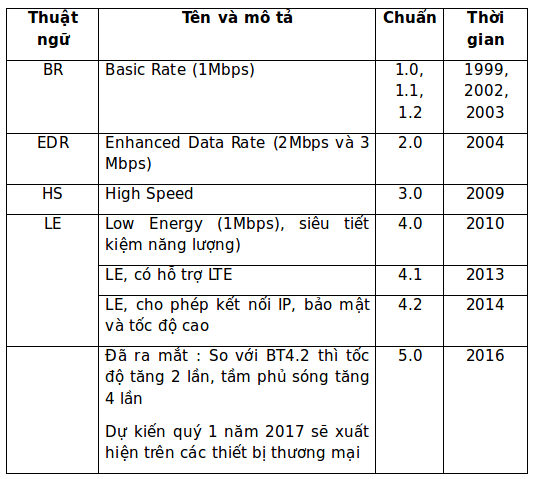
\includegraphics[width=0.7\linewidth]{graphics/lich_su_ble.png}
    \caption{Sự phát triển của công nghệ Bluetooth qua các thời kỳ}
\end{figure}

\subsubsection{Sự khác biệt của BLE}

Sự bùng nổ của các thiết bị thông minh hiện nay đã tạo ra nhu cầu tăng cao trong việc kết nối các thiết bị này với những nguồn bên ngoài. Trong bối cảnh đó, công nghệ Bluetooth Low Energy (BLE) đã được tích hợp vào hầu hết các mẫu điện thoại thông minh hiện đại.

\begin{itemize}
    \item BLE có chi phí thấp, điều này làm cho nó trở thành một lựa chọn hấp dẫn cho nhiều nhà sản xuất thiết bị.
    \item Công nghệ này cho phép các thiết bị giao tiếp hiệu quả với các nền tảng di động tiên tiến, giúp chúng dễ dàng trao đổi dữ liệu.
    \item Nhiều thiết bị chỉ cần truyền tải một lượng dữ liệu nhỏ trong mỗi lần kết nối và cần tiết kiệm pin, như thiết bị theo dõi nhịp tim hoặc thiết bị giám sát trẻ em, đều là những ví dụ tiêu biểu cho ứng dụng của BLE.
\end{itemize}

Ngoài ra, BLE cũng có mô hình dữ liệu tương đối đơn giản và không yêu cầu đầu tư vào giấy phép sử dụng, cùng với một stack giao thức không quá phức tạp, giúp việc phát triển trở nên dễ dàng hơn.

\subsubsection{Các kiểu thiết bị Bluetooth}

Tài liệu Bluetooth Specification (4.0 trở đi) định nghĩa hai công nghệ không dây sau:

\begin{itemize}
    \item BR/EDR (Classic Bluetooth)
    \item BLE (Bluetooth Low Energy)
\end{itemize}

Hiện nay các thiết bị Bluetooth được thể hiện trong hình sau:

\begin{figure} [!htp]
    \centering
    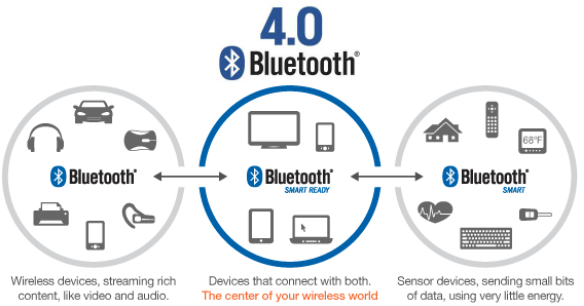
\includegraphics[width=0.8\linewidth]{graphics/cac_thiet_bi_blt.png}
    \caption{Các thiết bị Bluetooth phổ biến}
\end{figure}

Như hình ảnh trên cho thấy, thiết bị BLE được chia thành hai loại chính, đó là Bluetooth Smart và Bluetooth Smart Ready.

\begin{itemize}
    \item \textbf{Bluetooth Smart (Chế độ đơn)}: Loại thiết bị này chỉ có khả năng tương tác với các thiết bị khác thuộc nhóm Bluetooth Smart hoặc Bluetooth Smart Ready mà thôi. Điều này có nghĩa là nó không thể kết nối với các thiết bị sử dụng công nghệ Bluetooth cổ điển (Classic Bluetooth).
    \item \textbf{Bluetooth Smart Ready (Chế độ kép)}: Thiết bị này mang lại sự linh hoạt hơn khi có khả năng giao tiếp với nhiều loại thiết bị khác nhau. Nó không chỉ có thể kết nối với các thiết bị Bluetooth Smart và Bluetooth Smart Ready, mà còn hỗ trợ cả các thiết bị sử dụng công nghệ Classic Bluetooth. Nhờ vậy, người dùng có thể dễ dàng truy cập và sử dụng nhiều loại thiết bị khác nhau mà không gặp phải rào cản về công nghệ.
\end{itemize}

\subsubsection{Các khối chính của 1 thiết bị Bluetooth}

Trong một thiết bị Bluetooth luôn bao gồm 3 khối chức năng chính:

\begin{itemize}
    \item \textbf{Khối Application:} Là khối ứng dụng hỗ trợ người dùng giao tiếp với Bluetooth protocol stack.
    \item \textbf{Khối Host:} Các lớp phía trên của Bluetooth protocol stack.
    \item \textbf{Khối Controller:} Bao gồm các chức năng truyền nhận là lớp dưới của Bluetooth protocol stack.
\end{itemize}

\textit{(\textbf{Bluetooth Protocol Stack:} Bộ giao thức dạng stack cho phép các thiết bị Bluetooth thiết lập, kết nối, truyền nhận dữ liệu với nhau)}

Ba khối chức năng chính của 1 thiết bị Bluetooth có thể cấu hình theo các kiểu phần cứng khác nhau, hình bên dưới biểu diễn 3 kiểu cấu hình phần cứng chính:

\begin{figure}[!htp]
    \centering
    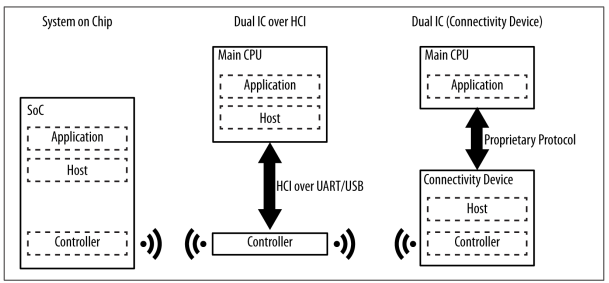
\includegraphics[width=0.8\linewidth]{graphics/phan_cung_bluetooth.png}
    \caption{Các kiểu cấu hình phần cứng chính của 1 thiết bị Bluetooth}
\end{figure}

\subsubsection{Các hạn chế của BLE}

\textbf{Thông lượng dữ liệu nhỏ}

Theo lý thuyết, trong không gian tần số điều chế của sóng BLE là 1Mbps. Tuy nhiên, tần số này có thể nhỏ hơn do tác động của nhiều yếu tố ngoại cảnh.

Ta đặt giả thiết là một thiết bị chủ (Master) được khởi tạo và thiết lập kết nối đến một ngoại vi (Slave) qua giao diện BLE:

\begin{itemize}
    \item Ta có khái niệm về chu kỳ kết nối (Conneciton interval), đây là khoảng thời gian giữa 2 sự kiện kết nối liên tiếp. Với BLE, khi một sự kiện kết nối diễn ra, các thiết bị trong kết nối sẽ trao đổi dữ liệu với nhau, sau đó trở về trạng thái IDLE để tiết kiệm năng lượng, và chờ đến thời điểm thì thực hiện sự kiện kết nối tiếp theo. Tham số này nằm trong khoảng 7.5ms đến 4s.
    \item nRF51822 có thể truyền đến 6 gói dữ liệu trong mỗi sự kiện kết nối. Mỗi gói có thể chứa 20 bytes dữ liệu của người dùng.
    \item Giả sử tần số sự kiện kết nối là lớn nhất (chu kỳ kết nối nhỏ nhất = 7.5ms). Khi đó mỗi giây có thể xảy ra tối đa 133 sự kiện kết nối
\end{itemize}

\textbf{Khoảng cách gần}

Các yếu tố ảnh hưởng đến khoảng cách truyền thông như môi trường hoạt động, thiết kế anten, vật cản, hướng thiết bị, ... BLE tập trung vào các ứng dụng truyền thông trong phạm vi gần.

Với BLE ta có:
\begin{itemize}
    \item Khoảng cách lý thuyết: 100m (điều kiện tốt).
    \item Khoảng cách khả thi: 30m.
    \item Khoảng cách thường được sử dụng: 2-5m.
\end{itemize}

\subsubsection{Protocols và Profiles}

Các thiết bị BLE cần tuân thủ một vài quy định để hai thiết bị có thể giao tiếp với nhau thông qua chuẩn BLE. Các quy định này được chia theo từng giao thức và cấu hình.

\textbf{Protocol} (Phương thức): Các định dạng gói tin, định tuyến, dồn kênh, mã hoá, . . . nhằm trao đổi thông tin giữa các bên được quy định trong Tập các lệnh.

\textbf{Profile} (Cấu hình): Định nghĩa cách mà giao thức được sử dụng nhằm thực hiện các mục đích cụ thể. Có hai loại cấu hình là cấu hình tổng quát (generic profiles) và cấu hình cụ thể theo trường hợp dùng (use-case profiles)


\begin{itemize}
    \item \textit{Generic profiles:} các profile cơ sở được mô tả trong tài liệu Bluetooth Specifications, đây là hai profiles không thể thiếu để các thiết bị BLE giao tiếp và chia sẻ thông tin với nhau, GAP và GATT.
    \item \textit{Use-case profile:} Các profile cho các trường hợp sử dụng cụ thể
    \begin{itemize}
        \item Các profile do Bluetooth Special Interest Group (SIG) định nghĩ
        \item Các profile do vendor tự định nghĩa
    \end{itemize}
\end{itemize}

\subsubsection{The BLE Protocols Stack}

\begin{figure}[!htp]
    \centering
    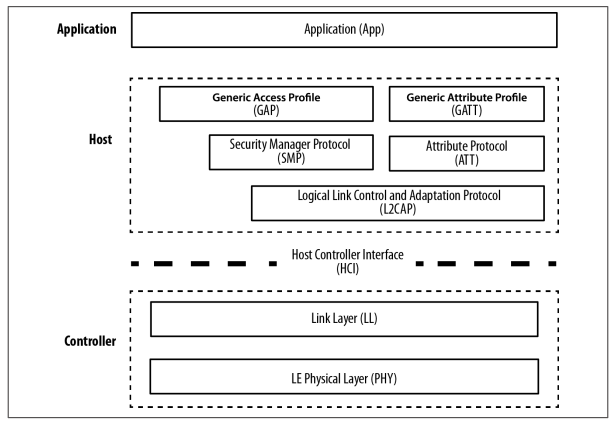
\includegraphics[width=0.8\linewidth]{graphics/cac_lop_ble.png}
    \caption{Các thành phần trong bộ giao thức BLE cơ bản}
\end{figure}

Bộ giao thức cho các thiết bị BLE được chia làm 3 thành phần chính: \textbf{Application}, \textbf{Host} và \textbf{Controller}

\textbf{Lớp Application:} Lớp cao nhất của cả giao thức cung cấp giao diện để giao tiếp với người dùng, xử lý logic, và điều khiển và tính toán dữ liệu liên quan đến ứng dụng. Tuỳ từng ứng dụng khác nhau mà có kiến trúc của lớp Application khác nhau.

\textbf{Lớp Host:} Bên trong lớp Host bao gồm các lớp con sau:
\begin{itemize}
    \item Generic Access Profile (GAP)
    \item Generic Attribute Profile (GATT)
    \item Attribute Protocol (ATT)
    \item Security Manager (SM)
    \item Logical Link Control and Adaptation Protocol (L2CAP)
    \item Host Controller Interface (HCI), Host side
\end{itemize}

\textbf{Lớp Controller:} Là lớp cuối cùng của cả bộ giao thức bên trong có chứa các lớp \textit{Host Controller Interface (HCI)}, \textit{Link Layer (LL)} và lớp \textit{LE Physical Layer}

\begin{figure}[!htp]
    \centering
    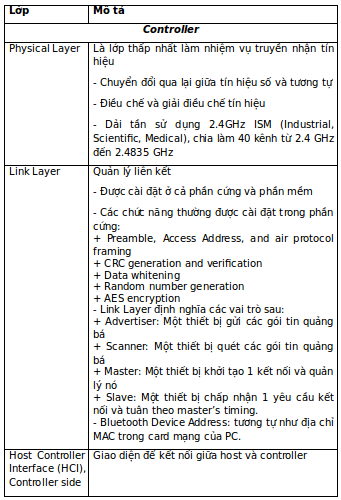
\includegraphics[width=0.5\linewidth]{graphics/lop_controller.png}
    \caption{Bảng mô tả chức năng của lớp Host}
\end{figure}

\begin{figure}[!htp]
    \centering
    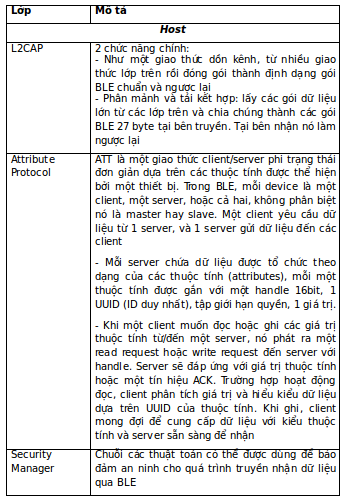
\includegraphics[width=0.5\linewidth]{graphics/lop_host.png}
    \caption{Bảng mô tả chức năng của lớp Controller}
\end{figure}

\begin{figure}[!htp]
    \centering
    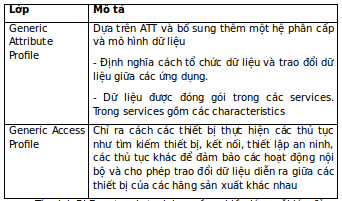
\includegraphics[width=0.5\linewidth]{graphics/GAP_GATT.png}
    \caption{Bảng mô tả chức năng của 2 profiles cơ sở: GAP và GATT}
\end{figure}

\subsubsection{GAP và GATT}

\textbf{GAP (Advertising and Connections):}

GAP (Generic Access Profile) là nền tảng cho phép các thiết bị BLE giao tiếp với nhau. Nó cung cấp một framework mà bất cứ thiết bị BLE nào cũng phải tuân theo để có thể tìm kiếm các thiết bị BLE (Bluetooth) khác, quảng bá dữ liệu, thiết lập kết nối an ninh, thực hiện nhiều hoạt động nền tảng theo một chuẩn.

Tài liệu BLE Specifications định nghĩa các khái niệm sau khi xét đến sự tương tác giữa các thiết bị:
\begin{itemize}
    \item Roles: Mỗi thiết bị có thể hoạt động theo một hoặc nhiều vai trò khác nhau tại cùng một thời điểm: broadcaster, observer, central, peripheral.
    \item Modes: Một mode là một trạng thái mà thiết bị có thể chuyển đến trong một khoảng thời gian để đạt được một mục đích cụ thể hoặc nhiều điều đặc biệt, để cho phép một peer thực hiện một thủ tục cụ thể.
    \item Procedures: Là các thủ tục (thường thì Link Layer điều khiển sự trao đổi gói tin) để cho phép một thiết bị đạt được một mục đích chắc chắn. Một thủ tục thường được liên kết với một mode, nên mode và procedure thường được xem xét cùng nhau.
    \item Security: GAP xây dựng dựa trên Security Manager và Security Manager Protocol (định nghĩa các modes và procedures an ninh để xác định cách mà các thiết bị đặt mức an ninh khi trao đổi dữ liệu). Ngoài ra GAP định nghĩa thêm các tính năng an ninh cao hơn mà không gắn với modes và procedures cụ thể nào, tăng cường mức bảo vệ dữ liệu được yêu cầu bởi mỗi ứng dụng.
\end{itemize}

\textbf{GATT (Services and Characteristics):}

GATT thiết lập chi tiết cách trao đổi tất cả profile và dữ liệu người dùng qua kết nối BLE. Ngược lại với GAP (định nghĩa sự tương tác mức thấp với các thiết bị), GATT chỉ trình bày các thủ tục truyền và định dạng dữ liệu thực tế

GATT sử dụng ATT và giao thức truyền của nó để trao đổi dữ liệu giữa các thiết bị. Dữ liệu này được tổ chức phân cấp thành các phần gọi là services, nó nhóm các phần khái niệm liên quan của dữ liệu người dùng gọi là characteristic. Nói một cách ngắn gọn thì dữ liệu truyền qua BLE là dữ liệu có cấu trúc, mà cụ thể là được tổ chức phân cấp thành services và characteristics.

\textbf{Roles}

\begin{itemize}
    \item GATT Client: tương ứng với ATT client, gửi yêu cầu đến server và nhận kết quả phản hồi. Ban đầu, GATT Client không biết server hỗ trợ những thuộc tính nào vì thế nó cần phải thực hiện service discovery.
    \item GATT Server: tương ứng ATT server, nhận yêu cầu từ client và gửi những nội dung tương ứng.
    \item Chú ý rằng các vai trò của GATT không phụ thuộc vào vai trò của GAP. Có nghĩa là cả GAP Central và GAP Peripheral có thể hoạt động như GATT Client hoặc GATT Server hoặc thậm chí là cả hai tại cùng một thời điểm.
\end{itemize}

\textbf{UUIDs}

\begin{itemize}
    \item Là một số định danh thiết bị, dài 128 bit (16 byte) duy nhất trên thế giới. Vì độ dài quá lớn, chiếm phần lớn trong gói dữ liệu, BLE Specification định nghĩa thêm 2 định dạng UUID: 16bit và 32 bit. Các định dạng ngắn này có thể chỉ được sử dụng với UUID được định nghĩa trong BT Specification.
\end{itemize}

\textbf{Attributes}

\begin{itemize}
    \item Là thực thể dữ liệu nhỏ nhất được định nghĩa bởi GATT (và ATT).
    \item Cả GATT và ATT chỉ làm việc với attributes nên để tương tác giữa client và server tất cả dữ liệu phải được tổ chức theo định dạng này.
    \item Mỗi attribute chứa thông tin về chính nó là dữ liệu người dùng và được mô tả như sau:
    \begin{itemize}
        \item Handle: số 16 bit duy nhất trên mỗi server để địa chỉ hóa attribute
        \item Type:là kiểu UUID, 16bit – 32bit – 128 bit
        \item Permission: xác định các ATT opertation có thể thực thi trên attribute cụ thể
        \item Value: chứa phần dữ liệu thực tế trong attribute, giới hạn 512 byte
    \end{itemize}
\end{itemize}

\textbf{Services và Characteristics}

Dữ liệu trao đổi thông qua kết nối BLE là dữ liệu có cấu trúc, được tổ chức phân cấp thành các services, bản thân services lại bao gồm các characteristics.

\newpage

\begin{figure}[!htp]
    \centering
    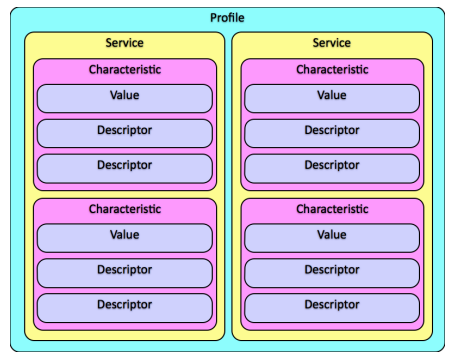
\includegraphics[width=0.6\linewidth]{graphics/ser_and_char.png}
    \caption{Services và Characteristics của BLE}
\end{figure}

\subsection{Cấu trúc dữ liệu được truyền từ cân sức khoẻ thông minh \cite{GATT:2024}}
Đặc tính Cân nặng được sử dụng để biểu thị cân nặng của một người dùng. Cấu trúc của đặc tính này được định nghĩa như sau:


\begin{table}[!htp]
    \centering
    \begin{tabular}{|>{\raggedright\arraybackslash}p{0.1\linewidth}|>{\raggedright\arraybackslash}p{0.1\linewidth}|>{\raggedright\arraybackslash}p{0.15\linewidth}|>{\raggedright\arraybackslash}p{0.65\linewidth}|} \hline 
         \textbf{Trường}&  \textbf{Loại dữ liệu}&  \textbf{Kích thước}
(trong octets)& \textbf{Mô tả}\\ \hline 
         Weight&  uint16&  2& Đơn vị cơ bản: org.bluetooth.unit.mass.kilogram. Giá trị biểu diễn: M = 5, d = -3, b = 0. Đơn vị là 0.005 kilogram\\ \hline
    \end{tabular}
    \caption{Cấu trúc của đặc tính Cân nặng (Weight characteristic)}
\end{table}

Đặc tính Đo lường Cân nặng được sử dụng để biểu thị dữ liệu liên quan đến việc đo lường cân nặng. Cấu trúc của đặc tính này được định nghĩa như sau:

\newpage

\begin{table} [!htp]
    \centering
    \begin{tabular}{|>{\raggedright\arraybackslash}p{0.1\linewidth}|>{\raggedright\arraybackslash}p{0.1\linewidth}|>{\raggedright\arraybackslash}p{0.15\linewidth}|>{\raggedright\arraybackslash}p{0.65\linewidth}|} \hline 
         \textbf{Trường}&  \textbf{Loại dữ liệu}&  \textbf{Kích thước}
(trong octets)& \textbf{Mô tả}\\ \hline 
         Flags&  boolean[8]&  1& Xem bảng mô tả ở dưới\\ \hline 
         Weight&  uint16&  2& Trường này được tính bằng kilogram với độ phân giải 0.005 nếu bit 0 của trường Cờ là 0, hoặc bằng pound với độ phân giải 0.01 nếu bit 0 của trường Flags là 1.\\ \hline 
         Time Stamp&  struct&  0 hoặc 7& Đơn vị là ngày với độ phân giải 1, giá trị nhỏ nhất: 1, giá trị lớn nhất: 16777214, giá trị biểu diễn: M = 1, d = 0, b = 0, đơn vị: org.bluetooth.unit.time.day, giá trị 0x000000 biểu thị 'value is not known'.\\ \hline 
         User ID&  uint8&  0 hoặc 1& Giá trị đặc biệt 0xFF cho User ID biểu thị "người dùng không xác định". Chức năng được enable nếu bit 2 của trường Flags được đặt thành 1.\\ \hline 
         BMI&  uint16&  0 hoặc 2& Đơn vị là 0.1 kg/m² hoặc org.bluetooth.unit.kilogram\_per\_square\_metre, giá trị biểu diễn: M = 1, d = -1, b = 0. Chức năng được enable nếu bit 3 của trường Flags được đặt thành 1.\\ \hline 
         Height&  uint16&  0 hoặc 2& Trường này được tính bằng mét với độ phân giải 0.001 nếu bit 0 của trường Flag là 0 hoặc bằng inch với độ phân giải 0.1 nếu bit 0 của trường Flag là 1. Chức năng được enable nếu bit 3 của trường Flags được đặt thành 1.\\ \hline
    \end{tabular}
    \caption{Cấu trúc của đặc tính Đo lường Cân nặng (Weight Measurement characteristic)}
\end{table}

Các bit của trường \textbf{Flags} được định nghĩa như sau:


\begin{table} [!htp]
    \centering
    \begin{tabular}{|>{\raggedright\arraybackslash}p{0.1\linewidth}|>{\raggedright\arraybackslash}p{0.9\linewidth}|} \hline 
         \textbf{Bit}& \textbf{Định nghĩa}\\ \hline 
         0& Các đơn vị đo lường: 0 = SI (Cân nặng và Khối lượng bằng đơn vị kilogram (kg) và Chiều cao bằng đơn vị mét); 1 = Imperial (Cân nặng và Khối lượng bằng đơn vị pound (lb) và Chiều cao bằng đơn vị inch (in)).\\ \hline 
         1& Time Stamp present\\ \hline 
         2& User ID present\\ \hline 
         3& BMI and Height present\\ \hline 
         4 - 7& Reserved for Future Use\\ \hline
    \end{tabular}
    \caption{Trường Flags}
\end{table}

\subsection{Thư viện Bleak}
\textbf{Bleak} là một thư viện Python hỗ trợ giao tiếp với các thiết bị Bluetooth Low Energy (BLE). Thư viện này rất phổ biến để kết nối với các thiết bị IoT (Internet of Things) hoặc các thiết bị BLE như đồng hồ thông minh, thiết bị theo dõi sức khỏe, và các thiết bị cảm biến. Các lớp được sử dụng trong dự án thuộc thư viện Bleak:

\subsubsection{Lớp BleakClient}
Đây là lớp đại diện cho kết nối BLE giữa thiết bị (laptop) và một thiết bị BLE khác. BleakClient cho phép thực hiện các thao tác chính như kết nối, đọc và viết dữ liệu, cũng như lắng nghe các thay đổi trong thuộc tính của thiết bị.

Ví dụ: Để kết nối và đọc thông tin từ một thiết bị BLE, BleakClient được sử dụng để thực hiện một kết nối ngắn hạn hoặc lâu dài.
\begin{lstlisting}[language=python,caption={Đoạn code mẫu sử dụng lớp BleakClient}]
import asyncio
from bleak import BleakClient

async def connect_device(address):
    async with BleakClient(address) as client:
        services = await client.get_services()
        for service in services:
            print(service)

asyncio.run(connect_device("device_ble_address"))
\end{lstlisting}

\subsubsection{Lớp BleakScanner}
Lớp này được sử dụng để quét các thiết bị BLE xung quanh. BleakScanner cho phép liệt kê các thiết bị BLE đang phát sóng trong phạm vi và trả về địa chỉ hoặc thông tin của thiết bị.

Ví dụ: Để quét và in ra danh sách các thiết bị BLE khả dụng:
\begin{lstlisting}[language=python,caption={Đoạn code mẫu sử dụng lớp BleakScanner}]
import asyncio
from bleak import BleakScanner

async def scan_devices():
    devices = await BleakScanner.discover()
    for device in devices:
        print(device)

asyncio.run(scan_devices())
\end{lstlisting}

\subsubsection{Lớp BleakGATTCharacteristic}
Đây là một lớp đại diện cho đặc tính (characteristic) của một dịch vụ GATT (Generic Attribute Profile) trên thiết bị BLE. Trong mô hình BLE, mỗi dịch vụ có thể có nhiều thuộc tính (characteristic), mỗi thuộc tính lại có thể chứa các giá trị cụ thể (như đo nhiệt độ, nhịp tim, v.v.).
\begin{itemize}
    \item Các characteristic thường được sử dụng để đọc, viết hoặc thông báo các thay đổi từ thiết bị BLE đến máy chủ (ví dụ: thiết bị BLE có thể tự động gửi thông tin nhịp tim khi giá trị này thay đổi).
\end{itemize}
Ví dụ, khi bạn đã kết nối với một thiết bị BLE và biết UUID của characteristic, bạn có thể đọc hoặc viết dữ liệu như sau:
\begin{lstlisting}[language=python,caption={Đoạn code mẫu sử dụng lớp BleakGATTCharacteristic}]
import asyncio
from bleak import BleakClient

async def read_characteristic(address, char_uuid):
    async with BleakClient(address) as client:
        value = await client.read_gatt_char(char_uuid)
        print(f"Value: {value}")

asyncio.run(read_characteristic("device_ble_address", "char_uuid"))
\end{lstlisting}

\subsection{Thư viện MediaPipe}
MediaPipe là một thư viện mã nguồn mở do Google phát triển, cho phép các nhà nghiên cứu và lập trình viên xây dựng các giải pháp và ứng dụng học máy tiên tiến trên nhiều nền tảng như di động, thiết bị biên, đám mây và web.

\textbf{Tính năng chính của MediaPipe:}

\begin{itemize}
    \item Xử lý đa phương tiện theo thời gian thực: MediaPipe hỗ trợ xử lý dữ liệu đa phương tiện như video, âm thanh và văn bản theo thời gian thực, phù hợp cho các ứng dụng yêu cầu độ trễ thấp và hiệu suất cao.
    \item Kiến trúc mô-đun linh hoạt: MediaPipe sử dụng kiến trúc dựa trên đồ thị, trong đó mỗi nút (được gọi là "Calculator") thực hiện một tác vụ cụ thể. Điều này cho phép dễ dàng tùy chỉnh và mở rộng các pipeline xử lý theo nhu cầu cụ thể của ứng dụng. \cite{mediapipe}
    \item Hỗ trợ đa nền tảng: Thư viện này có thể được triển khai trên nhiều hệ điều hành và nền tảng phần cứng khác nhau, bao gồm Windows, macOS, Linux và các thiết bị di động.
\end{itemize}

\textbf{Cài đặt MediaPipe trong Python:}

Để cài đặt MediaPipe, có thể sử dụng pip:

\begin{lstlisting}[language=python,caption={Đoạn code cài đặt thư viện MediaPipe}]
pip install mediapipe
\end{lstlisting}

Sau khi cài đặt, nhập thư viện vào dự án Python:

\begin{lstlisting}[language=python,caption={Đoạn code cài đặt thư viện MediaPipe}]
import mediapipe as mp
\end{lstlisting}

\textbf{Các giải pháp sẵn có trong MediaPipe:}

MediaPipe cung cấp nhiều giải pháp đã được xây dựng sẵn cho các tác vụ thị giác máy tính phổ biến, bao gồm: \cite{mediapipe}

\begin{itemize}
    \item Phát hiện và theo dõi khuôn mặt: Xác định vị trí và theo dõi các điểm đặc trưng trên khuôn mặt trong thời gian thực.
    \item Nhận diện cử chỉ tay: Phát hiện và theo dõi bàn tay, cùng với nhận diện các cử chỉ cụ thể. \cite{vohungvi}
    \item Phân tích tư thế cơ thể: Xác định vị trí của các khớp và bộ phận trên cơ thể người, hỗ trợ trong việc phân tích chuyển động và tư thế.
    \item Nhận diện đối tượng: Phát hiện và theo dõi các đối tượng trong video hoặc hình ảnh.
\end{itemize}

\textbf{Ứng dụng của MediaPipe:}

Nhờ vào khả năng xử lý mạnh mẽ và linh hoạt, MediaPipe được ứng dụng rộng rãi trong nhiều lĩnh vực, bao gồm:

\begin{itemize}
    \item \textbf{Thực tế tăng cường (AR):} Tạo các hiệu ứng AR dựa trên nhận diện khuôn mặt và cử chỉ tay.
    \item \textbf{Y tế:} Phân tích tư thế và chuyển động để hỗ trợ chẩn đoán và điều trị.
    \item \textbf{Thể thao:} Theo dõi và phân tích kỹ thuật của vận động viên trong thời gian thực. \cite{gfg_mediapipe}
    \item \textbf{Giải trí:} Tạo các ứng dụng tương tác dựa trên nhận diện cử chỉ và chuyển động.
\end{itemize}

MediaPipe là một công cụ mạnh mẽ và linh hoạt cho các dự án liên quan đến thị giác máy tính và học máy, cung cấp nhiều giải pháp sẵn có và khả năng tùy chỉnh cao, giúp tăng tốc quá trình phát triển và triển khai các ứng dụng thông minh.

\subsection{Giao thức MQTT}

\textbf{Message Queuing Telemetry Transport} (MQTT) là một giao thức truyền tin nhắn nhẹ dựa trên mô hình publish-subscribe, được thiết kế để kết nối các thiết bị trong môi trường mạng có băng thông thấp, độ trễ cao hoặc không ổn định. MQTT đặc biệt phù hợp cho các ứng dụng trong lĩnh vực Internet of Things (IoT), nơi các thiết bị thường có tài nguyên hạn chế và yêu cầu giao tiếp hiệu quả. \cite{emqx_mqtt}

\subsubsection{Nguyên lý hoạt động}

MQTT hoạt động theo mô hình publish-subscribe, trong đó:

\begin{itemize}
    \item \textbf{Publisher (Nhà xuất bản):} Gửi thông điệp đến một hoặc nhiều "chủ đề" (topics) cụ thể.
    \item \textbf{Subscriber (Người đăng ký):} Đăng ký nhận thông điệp từ một hoặc nhiều chủ đề quan tâm.
    \item \textbf{Broker (Máy môi giới):} Trung gian chịu trách nhiệm tiếp nhận thông điệp từ publisher và phân phối đến các subscriber tương ứng.
\end{itemize}

\begin{figure}[!htp]
    \centering
    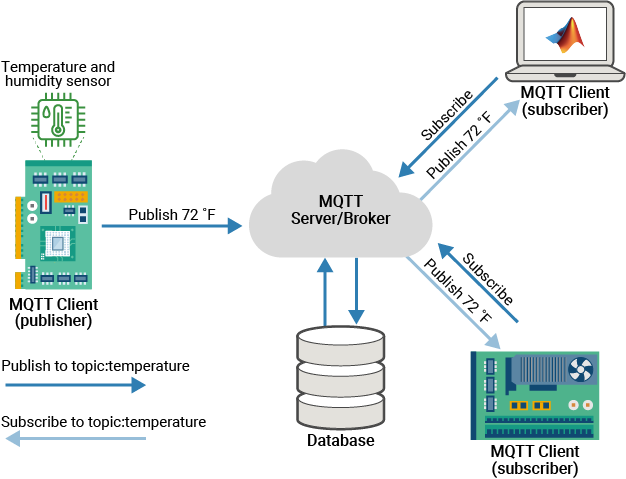
\includegraphics[width=0.75\linewidth]{graphics/mqtt_chart.png}
    \caption{Mô hình publish-subscribe của 1 MQTT}
\end{figure}

\subsubsection{Các mức chất lượng dịch vụ (QoS)}

MQTT hỗ trợ ba mức QoS để đảm bảo độ tin cậy trong việc truyền thông điệp: \cite{matlab_mqtt}

\begin{itemize}
    \item \textbf{QoS 0 (At most once):} Thường được gọi là "gửi rồi quên", là phương thức truyền tin theo cơ chế nỗ lực tối đa (best effort). Không có bất kỳ đảm bảo nào rằng thông điệp sẽ được gửi thành công. Bên nhận không xác nhận việc đã nhận được thông điệp, và bên gửi cũng không thực hiện gửi lại nếu thất bại, mà sẽ xóa thông điệp đó khỏi bộ nhớ cục bộ sau khi gửi.
\end{itemize}

\newpage

\begin{figure}[!htp]
    \centering
    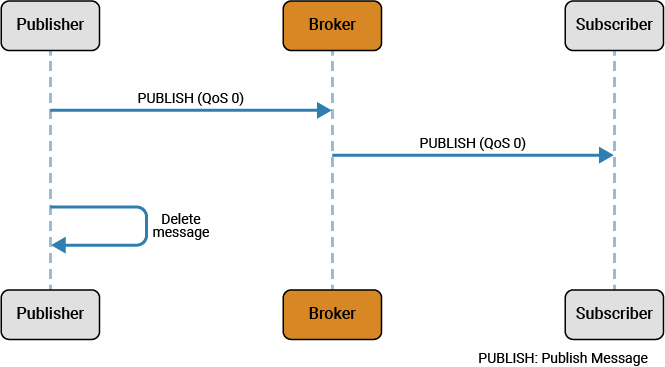
\includegraphics[width=0.75\linewidth]{graphics/qos0_mqtt.png}
    \caption{Mô hình publish-subscribe của mức QoS 0 (At most once)}
\end{figure}

\begin{itemize}
    \item \textbf{QoS 1 (At least once):} Đảm bảo rằng thông điệp sẽ được gửi đến ít nhất một lần. Bên gửi sẽ lưu trữ thông điệp cho đến khi nhận được gói xác nhận đã nhận (PUBACK) từ bên nhận. Nếu sau 10 giây không nhận được xác nhận, bên gửi sẽ thực hiện gửi lại thông điệp. Ở cấp độ này, một thông điệp có thể được gửi hoặc nhận nhiều lần.
\end{itemize}

\newpage

\begin{figure}[!htp]
    \centering
    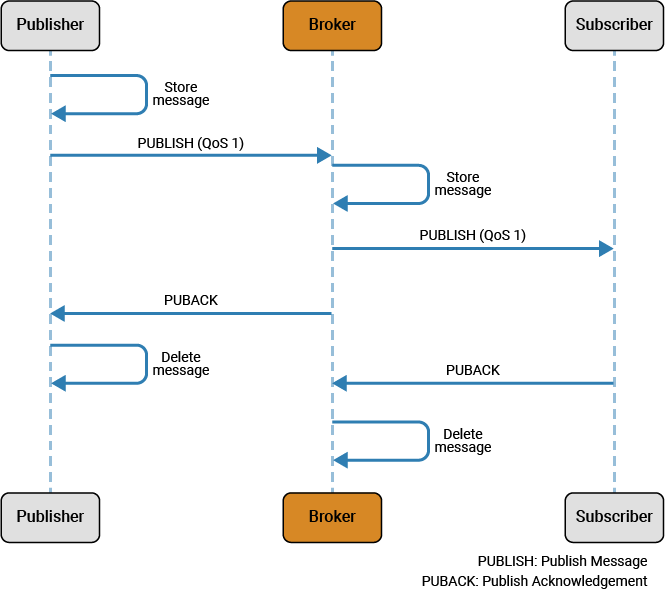
\includegraphics[width=0.75\linewidth]{graphics/qos1_mqtt.png}
    \caption{Mô hình publish-subscribe của mức QoS 1 (At least once)}
\end{figure}

\begin{itemize}
    \item \textbf{QoS 2 (Exactly once):} Là cấp độ dịch vụ cao nhất trong giao thức MQTT, mang đến sự đảm bảo rằng mỗi thông điệp chỉ được nhận một lần duy nhất bởi đúng đối tượng nhận. Tuy nhiên, để đạt được độ tin cậy này, QoS 2 đòi hỏi thêm chi phí xử lý do sử dụng quy trình bắt tay gồm bốn bước, khiến nó trở thành cấp độ chậm nhất trong ba mức QoS. Quá trình hoạt động của QoS 2 bắt đầu khi bên nhận tiếp nhận một gói tin PUBLISH. Sau khi xử lý nội dung thông điệp, bên nhận sẽ phản hồi bằng một gói xác nhận đã nhận, gọi là PUBREC. Trong trường hợp bên gửi không nhận được gói PUBREC, nó sẽ tiếp tục gửi lại gói PUBLISH cho đến khi nhận được phản hồi. Một khi gói PUBREC được nhận, bên gửi sẽ loại bỏ gói PUBLISH khỏi bộ nhớ, đồng thời lưu lại gói PUBREC và tiếp tục gửi một gói tin khác có tên là PUBREL để thông báo rằng quá trình gửi đã hoàn tất. Tiếp theo, khi bên nhận nhận được gói PUBREL, nó sẽ xóa mọi trạng thái liên quan đến thông điệp đang xử lý, và gửi lại một gói phản hồi cuối cùng là PUBCOMP. Ngay sau khi nhận được gói PUBCOMP, bên gửi sẽ xóa gói PUBREC đã lưu trước đó, đồng thời giải phóng mã định danh gói tin để có thể sử dụng lại cho các thông điệp tiếp theo. Thông qua quy trình này, QoS 2 đảm bảo mức độ tin cậy cao nhất, đồng thời tránh được việc gửi trùng lặp, vốn có thể xảy ra ở các cấp độ thấp hơn.
\end{itemize}

\begin{figure}[!htp]
    \centering
    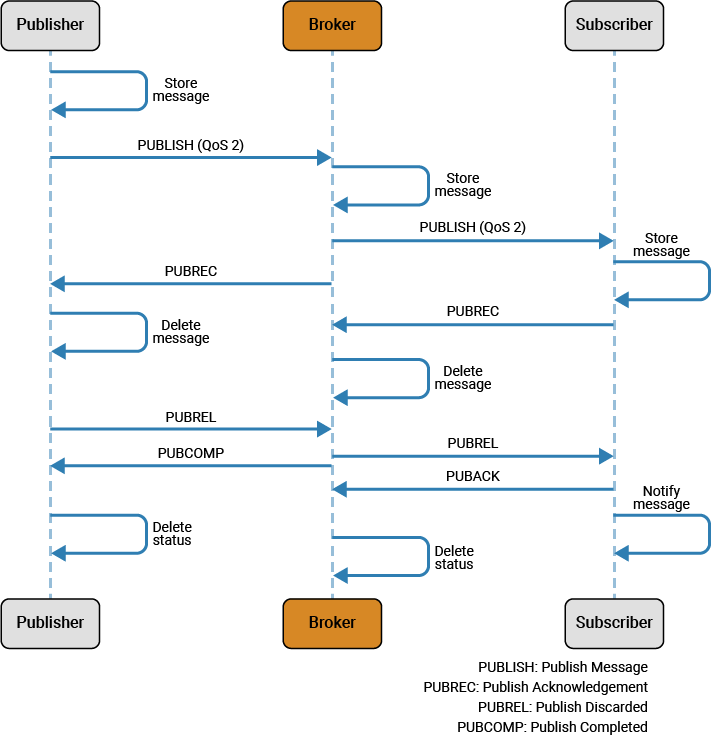
\includegraphics[width=0.75\linewidth]{graphics/qos2_mqtt.png}
    \caption{Mô hình publish-subscribe của mức QoS 2 (Exactly once)}
\end{figure}

\subsubsection{Ưu điểm của MQTT}

\begin{itemize}
    \item \textbf{Nhẹ và hiệu quả:} Thiết kế tối giản giúp giảm thiểu tài nguyên cần thiết, phù hợp với các thiết bị có khả năng xử lý và bộ nhớ hạn chế.
    \item \textbf{Độ tin cậy cao:} Các mức QoS cho phép lựa chọn giữa hiệu suất và độ tin cậy tùy theo yêu cầu ứng dụng.
    \item \textbf{Mở rộng linh hoạt:} Mô hình publish-subscribe cho phép dễ dàng mở rộng hệ thống và tích hợp nhiều thiết bị.
    \item \textbf{Hỗ trợ đa nền tảng:} MQTT có thể triển khai trên nhiều hệ điều hành và nền tảng phần cứng khác nhau.
\end{itemize}

\subsubsection{Ứng dụng của MQTT}

MQTT được sử dụng rộng rãi trong các lĩnh vực như:

\begin{itemize}
    \item \textbf{Nhà thông minh:} Điều khiển và giám sát các thiết bị gia dụng thông minh.
    \item \textbf{Công nghiệp:} Thu thập dữ liệu từ cảm biến và điều khiển thiết bị trong quy trình sản xuất.
    \item \textbf{Y tế:} Giám sát từ xa các thông số sức khỏe của bệnh nhân thông qua các thiết bị đeo.
    \item \textbf{Giao thông vận tải:} Theo dõi vị trí và trạng thái của phương tiện trong thời gian thực.
\end{itemize}

Với những đặc điểm trên, MQTT đã trở thành tiêu chuẩn phổ biến cho việc truyền thông tin trong các hệ thống IoT hiện đại.

\subsection{Nền tảng Core IoT}

Nền tảng Core IoT, truy cập tại \href{https://app.coreiot.io/}{Core IoT}, là một giải pháp công nghệ tiên tiến được thiết kế để hỗ trợ các kỹ sư lập trình nhúng trong việc quản lý, giám sát và vận hành các hệ thống IoT một cách hiệu quả. Được xây dựng dựa trên ThingsBoard – một nền tảng IoT mã nguồn mở nổi tiếng – Core IoT cung cấp các công cụ mạnh mẽ để thu thập, xử lý, trực quan hóa dữ liệu và quản lý thiết bị \cite{ThingsBoard}. Với khả năng hỗ trợ các giao thức chuẩn công nghiệp như MQTT, CoAP và HTTP, nền tảng này đảm bảo khả năng kết nối liền mạch và tương tác linh hoạt giữa các thiết bị IoT, đáp ứng nhu cầu đa dạng của các dự án IoT từ quy mô nhỏ đến lớn. Bài viết này sẽ phân tích chi tiết các tính năng chính, ứng dụng di động và khả năng tích hợp giao thức MQTT của Core IoT, đồng thời làm rõ vai trò của nền tảng trong việc tối ưu hóa quản lý hệ thống IoT.

\subsubsection{Tính năng chính của Core IoT}

Core IoT nổi bật với bộ tính năng toàn diện, được thiết kế để đáp ứng các yêu cầu phức tạp của quản lý và vận hành hệ thống IoT. Dưới đây là các tính năng cốt lõi của nền tảng, được trình bày một cách chi tiết:

\begin{enumerate}
    \item \textbf{Quản lý thiết bị và tài sản:} Core IoT cung cấp khả năng cung cấp, giám sát và điều khiển các thực thể IoT (thiết bị, tài sản, khách hàng) thông qua các API phía máy chủ mạnh mẽ. Người dùng có thể thiết lập các mối quan hệ giữa các thực thể, chẳng hạn như liên kết một nhóm thiết bị với một tài sản cụ thể hoặc một khách hàng, từ đó tạo ra một hệ thống quản lý linh hoạt và có tổ chức. Tính năng này đặc biệt hữu ích trong các ứng dụng như giám sát nhà máy thông minh hoặc quản lý đội xe, nơi cần theo dõi và điều phối nhiều thiết bị cùng lúc \cite{CoreIoT}.

    \item \textbf{Thu thập và trực quan hóa dữ liệu:} Nền tảng cho phép thu thập và lưu trữ dữ liệu từ xa một cách đáng tin cậy, với khả năng chịu lỗi và mở rộng cao. Dữ liệu được trực quan hóa thông qua hơn 30 widget tùy chỉnh, bao gồm biểu đồ đường, đồng hồ số, bản đồ và bảng, giúp người dùng xây dựng các bảng điều khiển (dashboard) phù hợp với nhu cầu cụ thể. Ví dụ, trong các ứng dụng giám sát môi trường, Core IoT có thể hiển thị dữ liệu từ các cảm biến nhiệt độ hoặc độ ẩm theo thời gian thực, hỗ trợ người dùng đưa ra quyết định nhanh chóng \cite{ThingsBoardDocs}.

    \item \textbf{Xử lý và phản ứng:} Core IoT tích hợp một công cụ quy tắc (rule engine) mạnh mẽ, cho phép định nghĩa các chuỗi xử lý dữ liệu phức tạp. Người dùng có thể chuyển đổi, chuẩn hóa dữ liệu từ thiết bị hoặc thiết lập các kịch bản tự động, chẳng hạn như kích hoạt cảnh báo khi phát hiện sự cố (ví dụ: thiết bị không hoạt động hoặc dữ liệu vượt ngưỡng). Tính năng này đảm bảo phản ứng kịp thời trước các tình huống bất thường, nâng cao hiệu quả vận hành của hệ thống IoT \cite{CoreIoT}.

    \item \textbf{Hỗ trợ triển khai linh hoạt:} Core IoT hỗ trợ cả triển khai trên đám mây (cloud) và tại chỗ (on-premises), phù hợp với các yêu cầu đa dạng của doanh nghiệp. Kiến trúc microservice của nền tảng đảm bảo khả năng mở rộng tuyến tính và tính chịu lỗi tối đa, cho phép hệ thống xử lý hàng triệu thiết bị mà không gặp gián đoạn. Điều này đặc biệt quan trọng trong các ứng dụng quy mô lớn như giám sát năng lượng thông minh hoặc quản lý đô thị thông minh \cite{ThingsBoardDocs}.

    \item \textbf{Bảo mật và quản lý quyền truy cập:} Nền tảng cung cấp các cơ chế bảo mật tiên tiến, bao gồm mã hóa dữ liệu trong quá trình truyền tải (hỗ trợ MQTT và HTTPS) và quản lý thông tin đăng nhập thiết bị dựa trên token hoặc chứng chỉ X.509. Ngoài ra, Core IoT áp dụng mô hình kiểm soát truy cập dựa trên vai trò (RBAC), cho phép phân quyền linh hoạt giữa các người dùng, đảm bảo an toàn và bảo mật dữ liệu trong toàn bộ hệ thống \cite{MQTT}.
\end{enumerate}

\newpage

\begin{figure}[!htp]
    \centering
    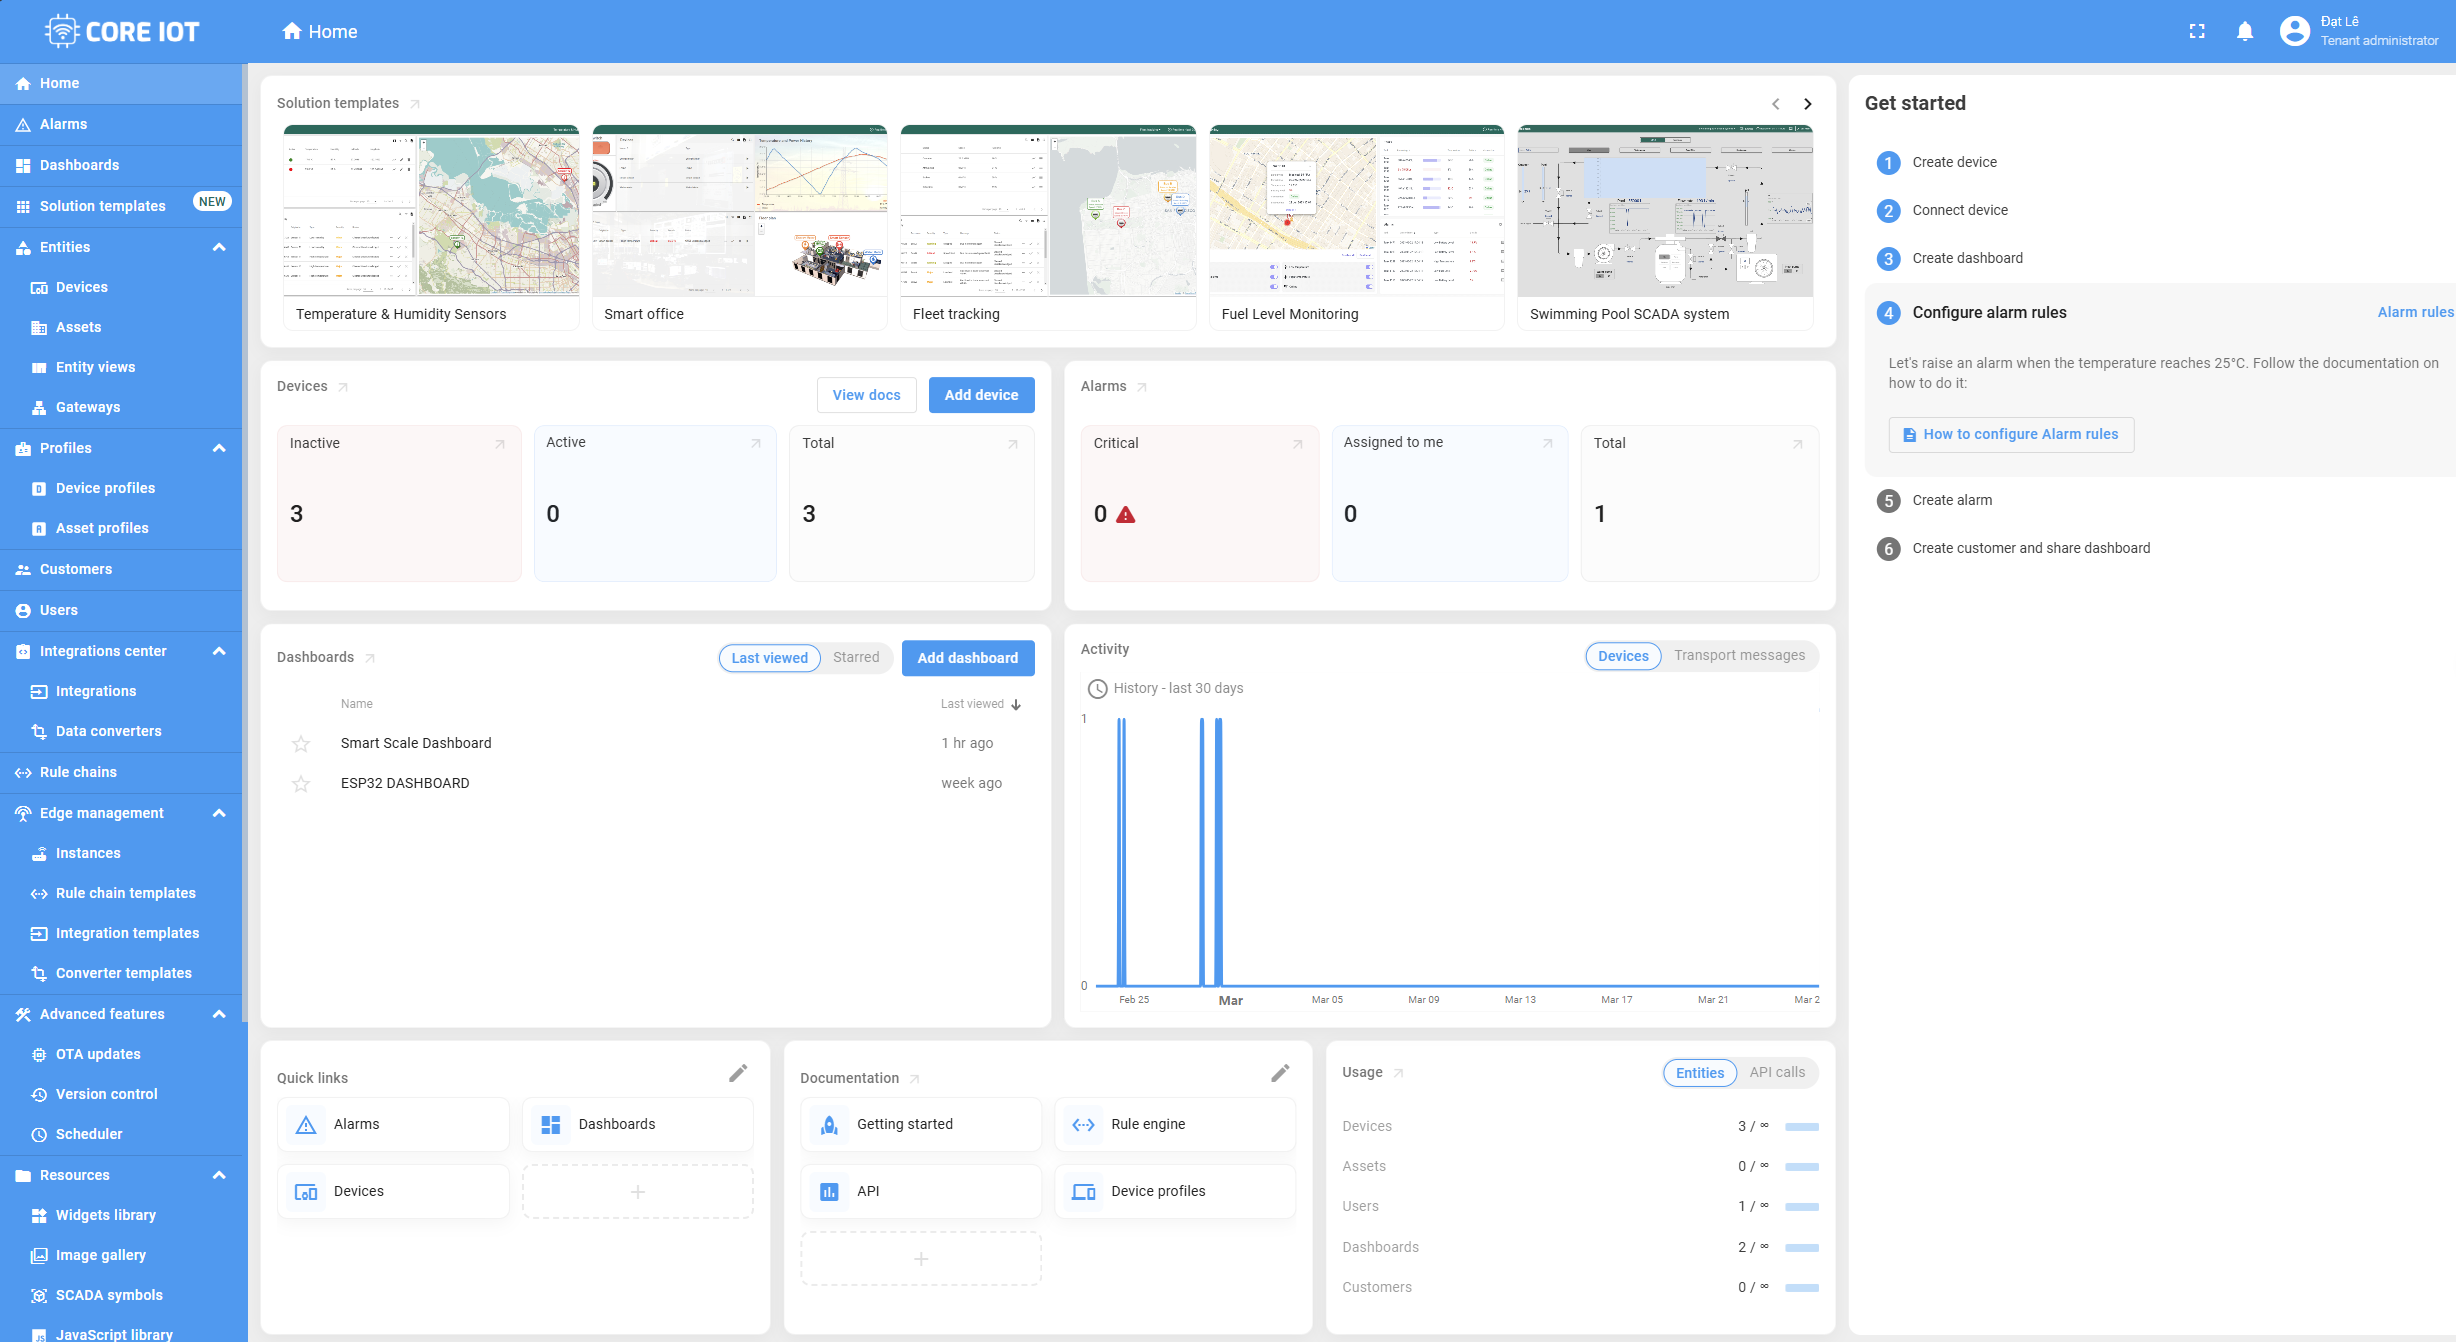
\includegraphics[width=0.9\linewidth]{graphics/giaodien_coreiot.png}
    \caption{Giao diện hệ thống Core IoT dành cho người dùng có quyền Tenant Administrator, hiển thị các công cụ quản lý và trực quan hóa dữ liệu.}
\end{figure}

\subsubsection{Ứng dụng di động Core IoT}

Để tăng cường tính tiện lợi và khả năng truy cập, Core IoT cung cấp một ứng dụng di động có sẵn trên Google Play Store, được phát triển dựa trên ứng dụng Flutter ThingsBoard mã nguồn mở. Ứng dụng này cho phép người dùng quản lý hệ thống IoT từ xa với các tính năng nổi bật sau:

\begin{itemize}
    \item \textbf{Quản lý bảng điều khiển:} Người dùng có thể duyệt, chỉnh sửa và tương tác với các bảng điều khiển được tùy chỉnh, giúp theo dõi trạng thái hệ thống IoT mọi lúc, mọi nơi.
    \item \textbf{Xử lý cảnh báo:} Ứng dụng hỗ trợ theo dõi và xử lý các cảnh báo liên quan đến thiết bị, chẳng hạn như thông báo về lỗi thiết bị hoặc dữ liệu bất thường, đảm bảo phản ứng nhanh chóng trước các sự cố.
    \item \textbf{Quản lý thiết bị theo hồ sơ:} Người dùng có thể quản lý các thiết bị theo từng hồ sơ cụ thể, phù hợp với các ứng dụng như giám sát tài sản hoặc quản lý đội xe.
    \item \textbf{Hành động di động:} Ứng dụng cho phép thực hiện các hành động được cấu hình trong các widget của bảng điều khiển, chẳng hạn như gửi lệnh điều khiển từ xa đến thiết bị.
\end{itemize}

Ứng dụng di động không chỉ mang lại sự linh hoạt mà còn tăng cường khả năng giám sát thời gian thực, đặc biệt trong các tình huống yêu cầu phản ứng nhanh, như quản lý hệ thống y tế thông minh hoặc giám sát cơ sở hạ tầng \cite{GooglePlayCoreIoT}.

\begin{figure}[!htp]
    \centering
    
\includegraphics[width=0.8\linewidth]{graphics/coreiot_chplay.png}
    \caption{Ứng dụng Core IoT trên Google Play Store, cung cấp khả năng quản lý IoT từ xa.}
\end{figure}

\subsubsection{Tích hợp giao thức MQTT trong Core IoT}

Giao thức MQTT (Message Queuing Telemetry Transport) là một trong những giao thức quan trọng được Core IoT tích hợp chặt chẽ, nhờ vào tính nhẹ, hiệu quả và khả năng hoạt động trong môi trường băng thông thấp. Sự tích hợp này mang lại các khả năng sau:

\begin{itemize}
    \item \textbf{Thu thập dữ liệu từ xa:} Các thiết bị IoT có thể gửi dữ liệu telemetry (như nhiệt độ, độ ẩm, hoặc vị trí) đến Core IoT thông qua các topic MQTT, đảm bảo việc thu thập dữ liệu liên tục và đáng tin cậy ngay cả trong điều kiện mạng không ổn định. Dữ liệu được lưu trữ an toàn và có thể truy cập thông qua API phía máy chủ hoặc bảng điều khiển \cite{MQTT}.
    \item \textbf{Quản lý thuộc tính thiết bị:} Core IoT cho phép thiết bị cập nhật các thuộc tính (attributes) của mình, chẳng hạn như trạng thái hoặc cấu hình, thông qua các topic MQTT được xác định trước. Đồng thời, máy chủ có thể gửi các cấu hình mới đến thiết bị, hỗ trợ quản lý từ xa hiệu quả \cite{ThingsBoardDocs}.
    \item \textbf{Thực hiện lệnh từ xa (RPC):} Nền tảng hỗ trợ giao tiếp hai chiều thông qua các lệnh RPC (Remote Procedure Call) dựa trên MQTT. Điều này cho phép máy chủ gửi các lệnh điều khiển đến thiết bị (ví dụ: bật/tắt thiết bị) và nhận phản hồi từ thiết bị, đảm bảo khả năng vận hành linh hoạt trong các ứng dụng như tự động hóa công nghiệp hoặc nhà thông minh \cite{MQTT}.
\end{itemize}

Việc tích hợp MQTT không chỉ tối ưu hóa hiệu suất truyền dữ liệu mà còn đảm bảo khả năng mở rộng và tính bảo mật, nhờ vào hỗ trợ mã hóa TLS trong quá trình truyền tải.
\section{BÁO CÁO KẾT QUẢ THỰC HIỆN}

\subsection{Tổng quan hệ thống}

Hệ thống chăm sóc sức khỏe điện tử được thiết kế nhằm cung cấp giải pháp theo dõi sức khỏe cá nhân tự động, sử dụng các thiết bị cân điện tử thông minh kết hợp với nền tảng IoT và trí tuệ nhân tạo (AI). Mục tiêu là tự động thu thập, phân tích và trực quan hóa các thông số sức khỏe, từ đó đưa ra các khuyến nghị hoặc cảnh báo phù hợp cho người dùng.

\subsubsection{Thành phần chính của hệ thống}

Hệ thống được chia thành các thành phần chức năng sau:

\begin{itemize}
  \item \textbf{Thiết bị cân sức khỏe thông minh (Xiaomi Smart Scale 2 / Crenot Gofit S2)}: Đóng vai trò thu thập dữ liệu cân nặng, chỉ số BIA (Bioelectrical Impedance Analysis) và truyền dữ liệu qua giao thức Bluetooth Low Energy (BLE).
  
  \item \textbf{Ứng dụng trung gian (máy tính cá nhân/điện thoại)}: Sử dụng thư viện \texttt{Bleak} để giao tiếp với thiết bị cân và nhận dữ liệu thô. Các chỉ số sau đó được phân tích, nội suy và xử lý tại đây.
  
  \item \textbf{Mô đun phân tích dữ liệu}: Áp dụng các công thức y sinh học và mô hình AI để tính toán các chỉ số như BMI, BMR, TDEE, LBM, phần trăm mỡ, tỷ lệ cơ – xương – nước trong cơ thể, đồng thời đưa ra các dự đoán và lời khuyên cá nhân hóa.
  
  \item \textbf{Hệ thống lưu trữ}: Dữ liệu sau khi xử lý được lưu trữ dưới định dạng \texttt{CSV}, phân loại theo từng người dùng, để phục vụ cho việc theo dõi sức khỏe dài hạn và đánh giá tiến trình thay đổi.
  
  \item \textbf{Nền tảng trực quan hoá (CoreIoT)}: Hệ thống cho phép đẩy dữ liệu theo thời gian thực thông qua giao thức MQTT lên nền tảng đám mây CoreIoT, nơi người dùng có thể giám sát các chỉ số sức khỏe qua giao diện bảng điều khiển (Dashboard).
\end{itemize}

\subsubsection{Quy trình hoạt động}

Quy trình hoạt động tổng thể của hệ thống được mô tả theo các bước sau:

\begin{enumerate}
  \item Người dùng thực hiện bước lên thiết bị cân thông minh.
  \item Dữ liệu được truyền qua BLE đến thiết bị xử lý trung gian.
  \item Ứng dụng xử lý dữ liệu, phân tích, nội suy và áp dụng các mô hình AI.
  \item Dữ liệu sau xử lý được lưu trữ và đẩy lên nền tảng CoreIoT.
  \item Người dùng theo dõi trực quan các thông số thông qua Dashboard và nhận khuyến nghị sức khỏe.
\end{enumerate}

\subsubsection{Sơ đồ kiến trúc hệ thống}

\begin{figure}[!htp]
    \centering
    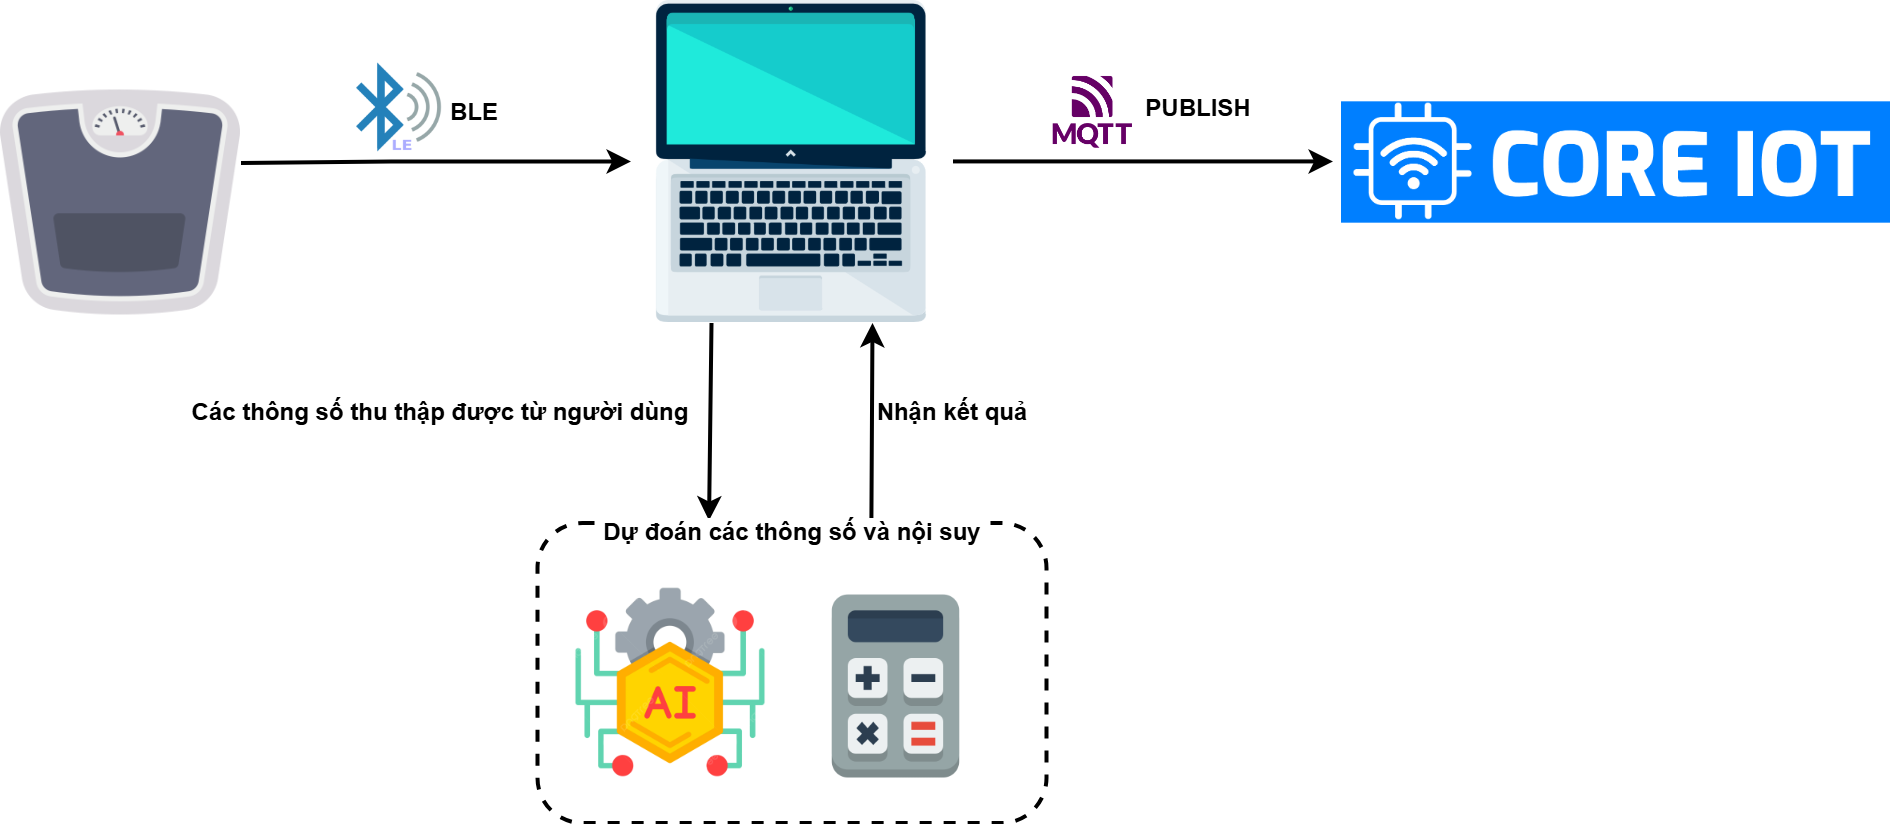
\includegraphics[width=0.9\linewidth]{graphics/scale_diagram.png}
    \caption{Sơ đồ kiến trúc hệ thống chăm sóc sức khỏe điện tử}
\end{figure}

Hình trên minh hoạ luồng dữ liệu và mối quan hệ giữa các thành phần trong hệ thống. Việc áp dụng kiến trúc phân tầng giúp đảm bảo tính mở rộng, dễ bảo trì và hỗ trợ tích hợp thêm các thiết bị mới hoặc dịch vụ y tế số trong tương lai.

\subsection{Thu thập các thông tin cơ bản từ người dùng}
Sử dụng thư viện \href{https://docs.python.org/3/library/tkinter.html}{Tkiner} của Python để tạo hộp thoại yêu cầu người dùng điền 1 số thông tin cá nhân cơ bản để phục vụ cho việc nội suy các chỉ số sức khoẻ.

\begin{figure} [!htp]
    \centering
    
\includegraphics[width=0.6\linewidth]{graphics/hopthoai.jpg}
    \caption{Hộp thoại được tạo bằng thư viện Tkiner để thu thập các thông tin cơ bản của người dùng}
\end{figure}

 Ở hộp thoại này, người dùng có thể nhập mới thông tin, hoặc chọn tên người dùng có sẵn được lưu trữ trước đó trong cơ sở dữ liệu, các thông tin còn lại như ngày sinh, chiều cao, và hệ số hoạt động sẽ được tự động điền.

\subsection{Đọc và phân tích dữ liệu cân nặng từ cân điện tử thông minh}
Đê có thể đọc và phân tích dữ liệu từ cân điện tử thông minh, đầu tiên ta phải biết được UUID của thiết bị. Để làm được điều đó em sử dụng ứng dụng trên điện thoại thông minh có tên "\textbf{BLE Scanner (Connect \& Notify)}" được tải từ CH Play.

\begin{figure} [!htp]
    \centering
    
\includegraphics[width=0.8\linewidth]{graphics/BLE Scanner.png}
    \caption{Ứng dụng BLE Scanner được tải từ CH Play}
\end{figure}

Sử dụng ứng dụng kết nối với 2 thiết bị cân thông  minh \textbf{Xiaomi Smart Scale 2} và \textbf{Crenot Gofit S2} để tìm UUID của 2 thiết bị.

\newpage

\begin{figure} [!htp]
    \centering
    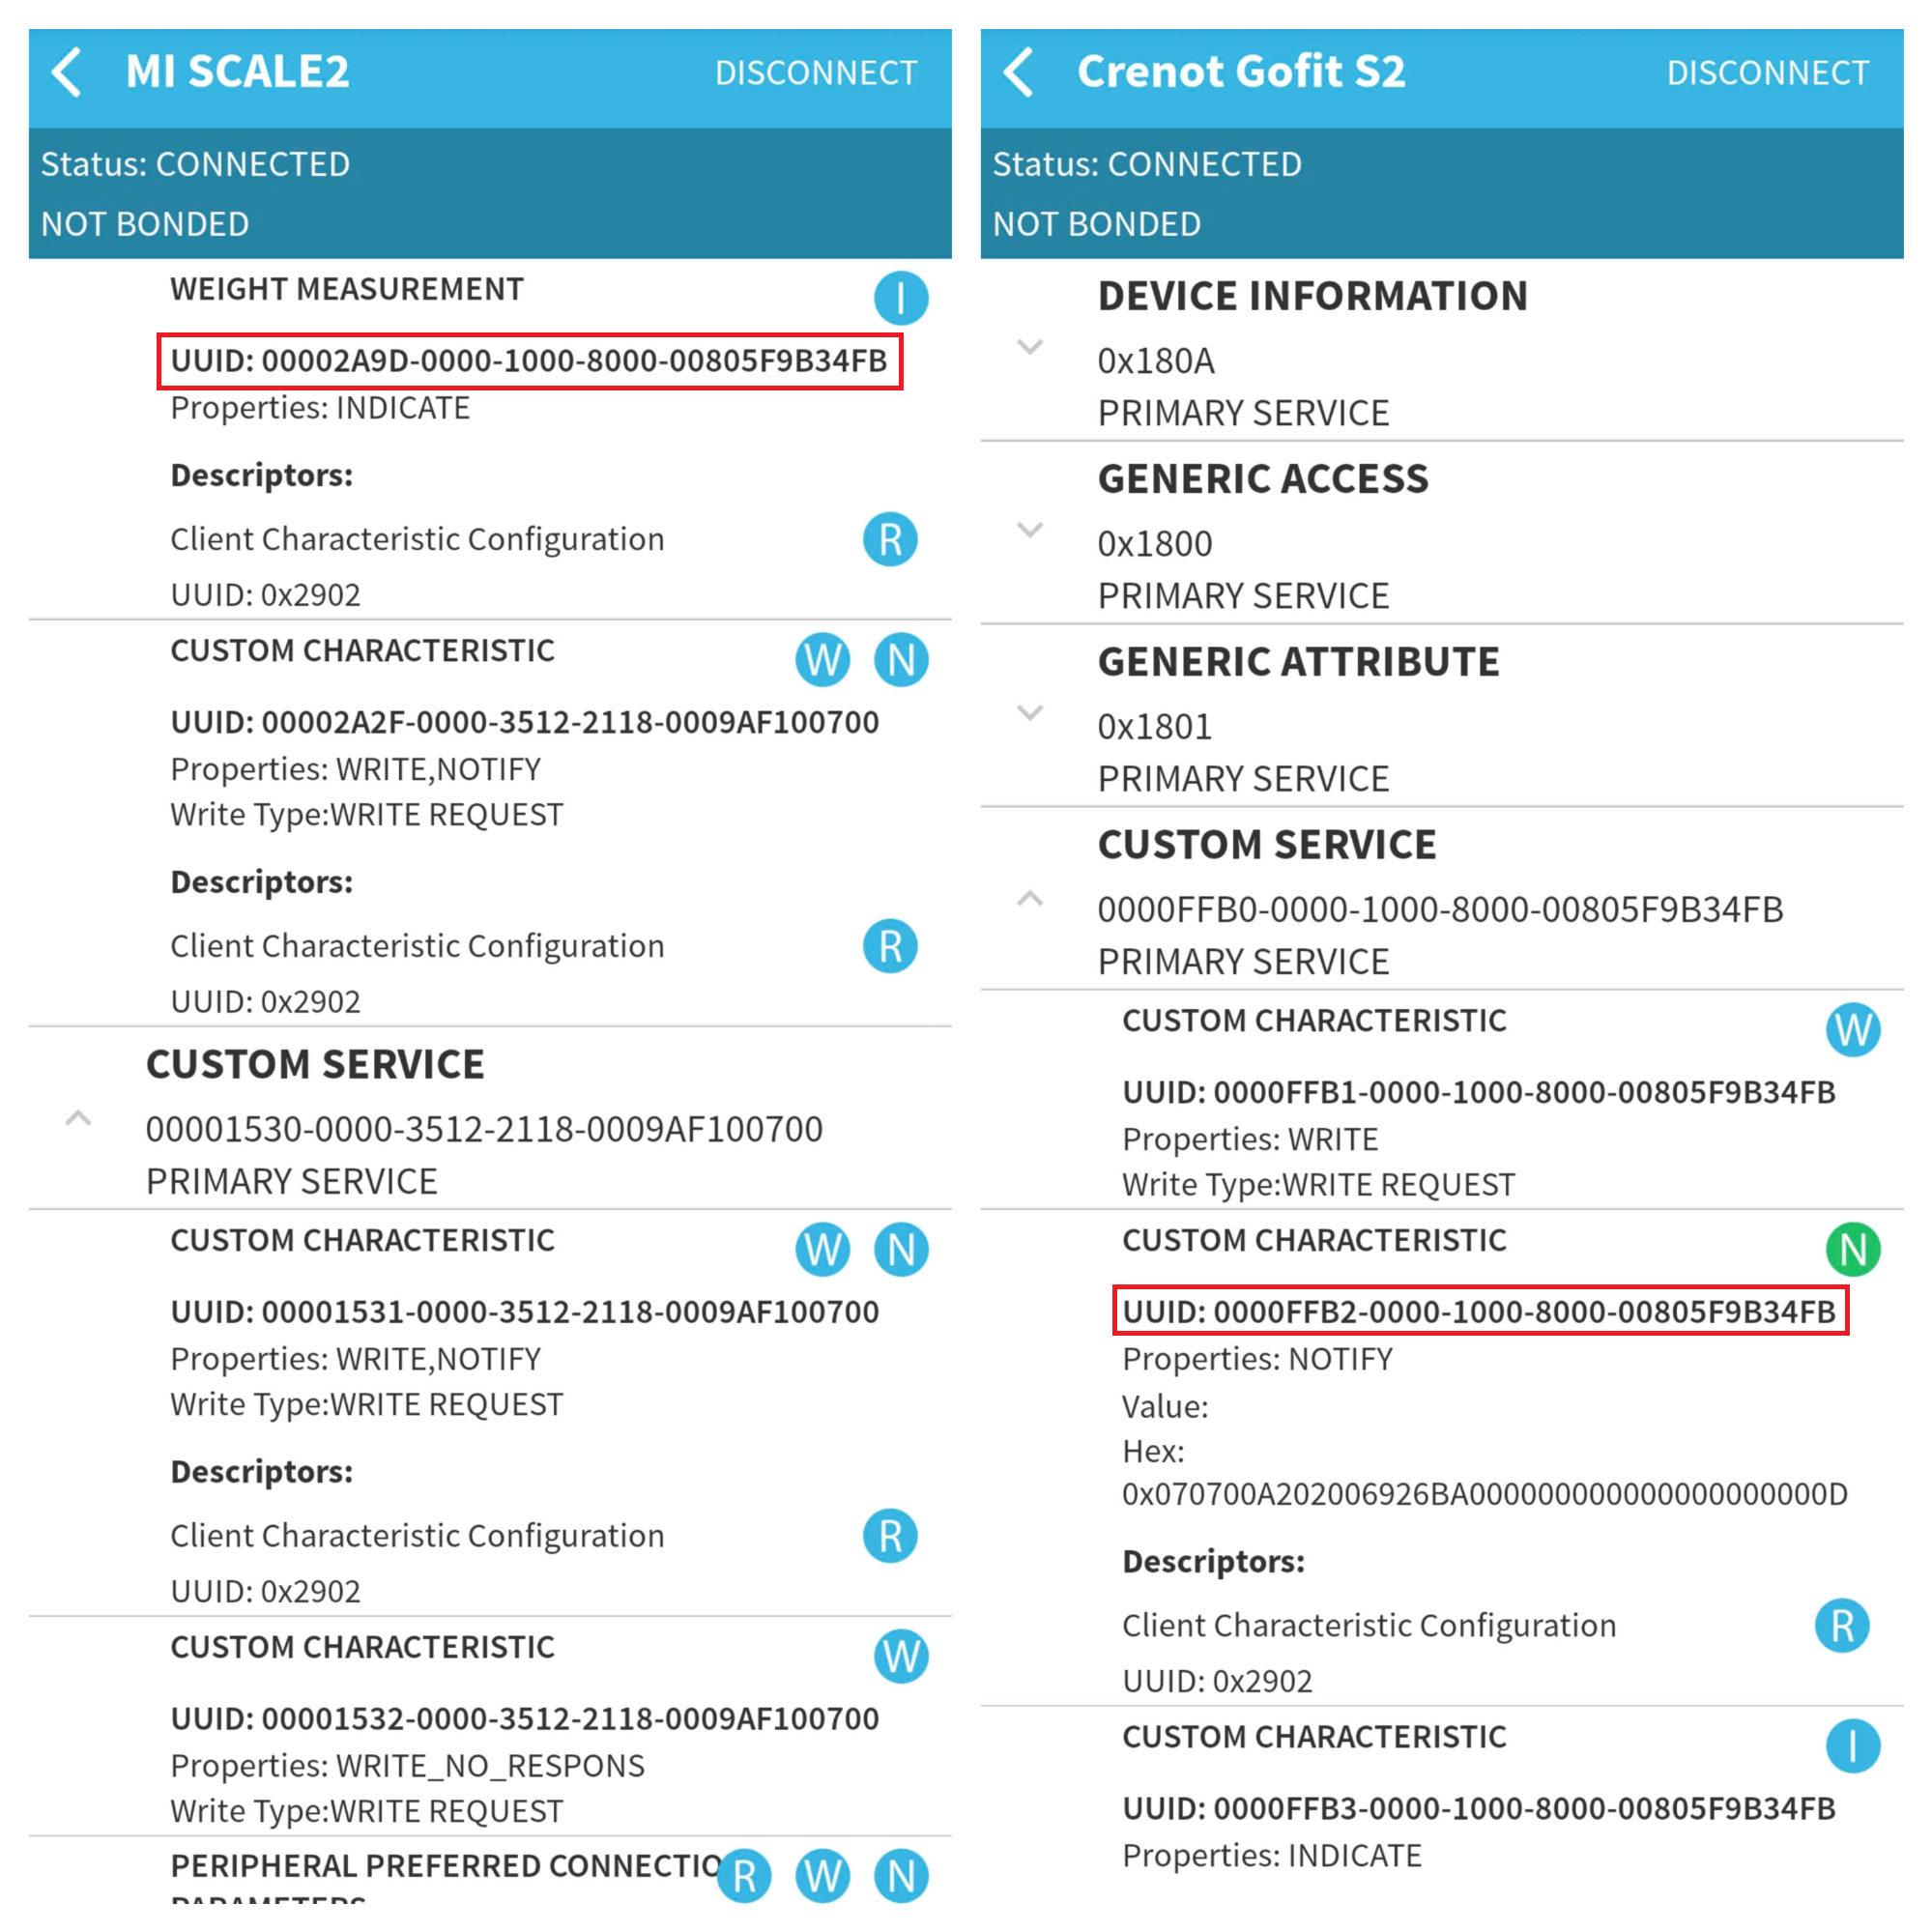
\includegraphics[width=0.6\linewidth]{graphics/miandcrenot.png}
    \caption{Tìm UUID của 2 thiết bị cân điện tử thông minh}
\end{figure}

Ta thu được 2 UUID tương ứng với 2 thiết bị Xiaomi Smart Scale 2 và Crenot Gofit S2 lần lượt như sau:

\begin{itemize}
    \item \textbf{Xiaomi Smart Scale 2 UUID:} 00002A9D-0000-1000-8000-00805F9B34FB
    \item \textbf{Crenot Gofit S2 UUID:} 0000FFB2-0000-1000-8000-00805F9B34FB
\end{itemize}

Sử dụng UUID vừa tìm được để kết nối với thiết bị cân cần nghiên cứu:

\begin{lstlisting}[language=python,caption={Sử dụng UUID để kết nối với thiết bị cần nghiên cứu}]
#DEVICE_NAME = 'MI SCALE2'
#BODY_COMPOSITION_MEASUREMENT_UUID = '00002A9D-0000-1000-8000-00805F9B34FB'  # UUID for the Weight Measurement
# characteristic Mi Scale 2

DEVICE_NAME = 'Crenot Gofit S2'
BODY_COMPOSITION_MEASUREMENT_UUID = '0000FFB2-0000-1000-8000-00805F9B34FB'  # UUID for the Weight Measurement
# characteristic Crenot Gofit S2

async def connect_and_measure():
    disconnected_event = asyncio.Event()

    def disconnected_callback(_bleak_client: BleakClient):
        logger.info("disconnected callback")
        disconnected_event.set()

    device = await find_scale_device()
    if device:
        logger.info(f"found device: {device.name}")
    if not device:
        logger.info("no device found")
        return

    client = BleakClient(device, disconnected_callback = disconnected_callback)

    async with client:
        await client.start_notify(
            BODY_COMPOSITION_MEASUREMENT_UUID, notification_handler
        )
        await disconnected_event.wait()
\end{lstlisting}

\subsubsection{Phân tích dữ liệu được gửi về từ Xiaomi Smart Scale 2}

Sử dụng đoạn code sau để phân tích dữ liệu từ cân Xiaomi ra chỉ số cân nặng có thể đọc được

\begin{lstlisting}[language=python,caption={Code phân tích dữ liệu cân nặng được gửi về từ cân Xiaomi}]
weight = int.from_bytes(data[1:3], byteorder = 'little')/200
\end{lstlisting}

Cụ thể:

\begin{itemize}
    \item data[1:3]: Lấy phần tử thứ 2 và thứ 3 (vì chỉ số bắt đầu từ 0) từ mảng data. Đoạn này là một mảng con chứa hai byte.
    \item int.from\_bytes(..., byteorder='little'): Chuyển đổi hai byte vừa lấy thành một số nguyên, sử dụng thứ tự byte là 'little\-endian' (byte nhỏ nhất nằm ở trước).
    \item / 200: Chia giá trị nguyên đó cho 200 để chuyển đổi thành một giá trị thập phân (theo lý thuyết về dữ liệu được gửi từ thiết bị BLE được trình bày phía trên).
\end{itemize}

\subsubsection{Phân tích dữ liệu được gửi về từ Crenot Gofit S2}

Để tìm được cân nặng được gửi từ thiết bị ta tiến hành khảo sát bằng cách cân thử và đọc dữ liệu gốc (dạng Hex) từ ứng dụng BLE Scanner ta thu được dữ liệu trả về trên ứng dụng như sau:

\begin{itemize}
    \item 76,7 kí: 0XCD0700A202006\textbf{92B9C}000000000000000000001A
    \item 0 kí: 0X3B0700A201006\textbf{80000}000000000000000000000B
\end{itemize}

Nhận thấy dữ liệu gốc trả về tương đồng nhau, chỉ khác nhau ở các phần tử 92B9C (76,6 kí) và 80000 (0 kí). Lấy 2 phần khác nhau trừ nhau ta thu được: 0x92B9C - 0x80000 = 0x12B9C đổi sang hệ DEC ta được 76700. Từ khảo sát trên ta có đoạn code tổng quát để xử lý dữ liệu được gửi về từ cân Crenot Gofit S2 như sau:

\begin{lstlisting}[language=python,caption={Code phân tích dữ liệu cân nặng được gửi về từ cân Crenot Gofit S2}]
weight = round((int(data.hex()[13:18], 16) - 524288) / 1000, 2)
\end{lstlisting}

\subsection{Nội suy các thông số sức khoẻ của cơ thể từ chỉ số cân nặng thu được}
Chỉ số cân nặng thu được từ cân điện tử, có thể được sử dụng để tính toán các thông số sức khoẻ khác của cơ thể dựa theo \href{https://github.com/lolouk44/xiaomi_mi_scale}{các công thức từ ứng dụng Mi Fit của Xiaomi}

\subsubsection{Chỉ số BMI}
Chỉ số BMI (Body Mass Index) là một công cụ được sử dụng để đánh giá mối quan hệ giữa cân nặng và chiều cao của một người, nhằm xác định xem họ có thuộc mức cân nặng bình thường, thừa cân hay thiếu cân hay không. Công thức tính BMI được thực hiện bằng cách lấy cân nặng (kg) chia cho bình phương chiều cao (m). Chỉ số BMI được tính trong project này thông qua hàm như sau:

\begin{lstlisting}[language=python,caption={Hàm tính toán chỉ số BMI của cơ thể}]
def get_bmi(height, weight):
    height_in_meters = height / 100
    return round(weight / (height_in_meters ** 2), 2)
\end{lstlisting}

Ngoài ra, dựa vào chỉ số BMI ta có thể chia ra các tình trạng thể chất như:
\begin{itemize}
    \item BMI < 18.5: Thiếu cân
    \item 18.5 $\leq$ BMI < 24.9: Bình thưởng
    \item 25 $\leq$ BMI < 29.9: Thừa cân
    \item BMI $\geq$ 30: Béo phì
\end{itemize}

\begin{lstlisting}[language=python,caption={Hàm đánh giá chỉ số BMI của cơ thể}]
def evaluate_bmi(bmi, height, weight):
    if bmi < 18.5:
        weight_needed = 18.5 * (height / 100) ** 2 - weight
        # bmi_eval_label.config(fg="blue", font=("Helvetica", 12, "bold"))
        return f"THIEU CAN, BAN CAN TANG KHOANG {weight_needed:.2f} kg."
    elif 18.5 <= bmi < 24.9:
        # bmi_eval_label.config(fg="green", font=("Helvetica", 12, "bold"))
        return "BINH THUONG"
    elif 25 <= bmi < 29.9:
        weight_needed = weight - 24.9 * (height / 100) ** 2
        # bmi_eval_label.config(fg="orange", font=("Helvetica", 12, "bold"))
        return f"THUA CAN, BAN CAN GIAM KHOANG {weight_needed:.2f} kg."
    else:
        weight_needed = weight - 24.9 * (height / 100) ** 2
        # bmi_eval_label.config(fg="red", font=("Helvetica", 12, "bold"))
        return f"BEO PHI. BAN CAN GIAM KHOANG {weight_needed:.2f} kg."
\end{lstlisting}

\subsubsection{Chỉ số TDEE và BMR}
Chỉ số BMR (Basal Metabolic Rate) là lượng calo cơ thể cần để duy trì các chức năng sống cơ bản như hô hấp, tuần hoàn và duy trì nhiệt độ cơ thể khi ở trạng thái nghỉ ngơi hoàn toàn. Đây là yếu tố quan trọng để xác định mức năng lượng tối thiểu cần thiết mỗi ngày.


Chỉ số TDEE (Total Daily Energy Expenditure) là lượng calo mà cơ thể cần để duy trì các hoạt động hàng ngày, bao gồm các hoạt động thể chất và sinh hoạt. TDEE được tính dựa trên BMR và hệ số hoạt động, giúp xác định lượng calo cần thiết để duy trì cân nặng hiện tại hoặc điều chỉnh chế độ ăn uống.

\begin{lstlisting}[language=python,caption={Hàm tính toán chỉ số TDEE và BMR của cơ thể}]
def get_bmr_tdee(weight, height, age, gender, activity_factor):
    if gender == 'male':
        bmr = 88.362 + (13.397 * weight) + (4.799 * height) - (5.677 * age)
    else:
        bmr = 447.593 + (9.247 * weight) + (3.098 * height) - (4.330 * age)
    tdee = bmr * activity_factor
    return round(bmr, 2), round(tdee, 2)
\end{lstlisting}

\subsubsection{Khối lượng cơ thể không mỡ (LBM)}
Chỉ số LBM (Lean Body Mass) hay khối lượng cơ thể không mỡ là một chỉ số thể hiện tổng khối lượng cơ bắp, xương, nước và các mô khác trong cơ thể, không bao gồm mỡ. Đây là một chỉ số quan trọng trong việc đánh giá thành phần cơ thể và theo dõi sức khỏe cũng như hiệu quả của các chương trình tập luyện.

\begin{lstlisting}[language=python,caption={Hàm tính toán chỉ số LBM của cơ thể}]
def get_lbm(height, weight, gender):
    if gender == 'male':
        lbm = (0.32810 * weight) + (0.33929 * height) - 29.5336
        return round(lbm, 2)
    else:
        lbm = (0.29569 * weight) + (0.41813 * height) - 43.2933
        return round(lbm, 2)
\end{lstlisting}

\subsubsection{Tỷ lệ phần trăm nước trong cơ thể}
Đoạn mã dưới đây được thiết kế để tính toán tỷ lệ phần trăm nước trong cơ thể dựa trên các thông tin cá nhân bao gồm giới tính, tuổi, cân nặng và chiều cao. Phương pháp này đóng vai trò quan trọng trong việc đánh giá sức khỏe và thể chất, bởi tỷ lệ nước trong cơ thể ảnh hưởng trực tiếp đến nhiều chức năng sinh lý. Để thực hiện điều này, đoạn mã sử dụng một công thức cơ bản dựa trên tỷ lệ phần trăm mỡ trong cơ thể, sau đó điều chỉnh kết quả bằng một hệ số phù hợp và đảm bảo giá trị cuối cùng nằm trong phạm vi hợp lý về mặt sinh lý học.

Trước tiên, tỷ lệ nước ban đầu được tính toán thông qua công thức sau:
\[
P_{\text{water}} = \left(100 - P_{\text{fat}}(G, A, W, H)\right) \times 0.7
\]
Trong đó, \( P_{\text{fat}}(G, A, W, H) \) biểu thị tỷ lệ phần trăm mỡ trong cơ thể, được xác định dựa trên giới tính (\(G\)), tuổi (\(A\)), cân nặng (\(W\)) và chiều cao (\(H\)) thông qua hàm \texttt{get\_fat\_percentage}. Công thức này xuất phát từ giả định rằng phần không có mỡ của cơ thể (lean body mass) chiếm khoảng 70\% là nước, do đó, sau khi trừ đi tỷ lệ mỡ, phần còn lại được nhân với 0.7 để ước lượng lượng nước.

Tiếp theo, giá trị \( P_{\text{water}} \) được tinh chỉnh bằng một hệ số điều chỉnh (coefficient), phụ thuộc vào mức nước ban đầu:
\[
\text{Coefficient} = 
\begin{cases} 
1.02 & \text{nếu } P_{\text{water}} \leq 50 \\
0.98 & \text{nếu } P_{\text{water}} > 50
\end{cases}
\]
Hệ số này được áp dụng nhằm phản ánh chính xác hơn tỷ lệ nước thực tế, có thể dựa trên các nghiên cứu thực nghiệm hoặc dữ liệu sinh lý. Sau khi xác định hệ số, đoạn mã kiểm tra một điều kiện đặc biệt: nếu \( P_{\text{water}} \times \text{coefficient} \geq 65 \), tỷ lệ nước sẽ được đặt thành 75. Bước này dường như là một cơ chế giới hạn giá trị tối đa, nhằm tránh các kết quả không hợp lý về mặt sinh học. Sau đó, giá trị \( P_{\text{water}} \) được nhân với hệ số và làm tròn đến hai chữ số thập phân để tăng độ chính xác và dễ đọc.

Cuối cùng, kết quả được đưa qua hàm \texttt{check\_val\_overflow} để đảm bảo nằm trong khoảng từ 35 đến 75, một phạm vi được coi là hợp lý về mặt sinh lý học:
\[
P_{\text{water, final}} = \text{CheckValOverflow}(P_{\text{water, adjusted}}, 35, 75)
\]
Hàm này có thể được hiểu là một bước kiểm tra và điều chỉnh, giới hạn giá trị để tránh vượt quá ngưỡng tối thiểu hoặc tối đa cho phép.

Dưới đây là mã nguồn Python minh họa quá trình tính toán:

\begin{lstlisting}[language=python,caption={Hàm tính toán chỉ số phần trăm nước của cơ thể}]
def get_water_percentage(gender, age, weight, height):
    water_percentage = (100 - get_fat_percentage(gender, age, weight, height)) * 0.7

    if water_percentage <= 50:
        coefficient = 1.02
    else:
        coefficient = 0.98

    # Capping water percentage
    if water_percentage * coefficient >= 65:
        water_percentage = 75

    water_percentage = water_percentage * coefficient
    water_percentage = round(water_percentage, 2)

    return check_val_overflow(water_percentage, 35, 75)
\end{lstlisting}

Cụ thể, quá trình triển khai trong mã nguồn bao gồm các bước sau:  
\begin{enumerate}
    \item Tính toán tỷ lệ nước ban đầu bằng cách lấy 100 trừ đi tỷ lệ mỡ (từ hàm \texttt{get\_fat\_percentage}), sau đó nhân với 0.7.  
    \item Xác định hệ số điều chỉnh dựa trên ngưỡng 50 của tỷ lệ nước ban đầu.  
    \item Áp dụng điều kiện giới hạn: nếu tích của tỷ lệ nước và hệ số lớn hơn hoặc bằng 65, giá trị được đặt thành 75.  
    \item Nhân tỷ lệ nước với hệ số và làm tròn kết quả đến hai chữ số thập phân.  
    \item Kiểm tra và điều chỉnh giá trị cuối cùng thông qua hàm \texttt{check\_val\_overflow} để đảm bảo nằm trong khoảng 35 đến 75.
\end{enumerate}

Như vậy, thông qua việc kết hợp công thức toán học và các bước xử lý trong mã nguồn, đoạn mã này cung cấp một phương pháp tính toán tỷ lệ nước trong cơ thể một cách có hệ thống, đồng thời đảm bảo tính chính xác và hợp lý về mặt khoa học.

\subsubsection{Khối lượng xương}

Đoạn mã được thiết kế nhằm tính toán khối lượng xương (\textit{bone mass}) dựa trên các thông tin cá nhân như chiều cao, cân nặng và giới tính. Phương pháp này đóng vai trò quan trọng trong việc đánh giá sức khỏe xương, một yếu tố cốt lõi ảnh hưởng đến sức khỏe tổng thể và khả năng vận động. Để thực hiện, đoạn mã sử dụng một công thức tích hợp giá trị cơ sở khác biệt giữa nam và nữ, kết hợp với khối lượng cơ thể không mỡ (LBM), sau đó tinh chỉnh và giới hạn kết quả để đảm bảo tính hợp lý về mặt sinh lý học.

Trước hết, giá trị cơ sở \( B_{\text{base}} \) được xác định dựa trên giới tính như sau:
\[
B_{\text{base}} = 
\begin{cases} 
0.245691014 & \text{(nữ)} \\
0.18016894 & \text{(nam)}
\end{cases}
\]
Giá trị này phản ánh sự khác biệt sinh học trong cấu trúc xương giữa hai giới. Tiếp theo, khối lượng cơ thể không mỡ (LBM) được tính toán thông qua hàm \texttt{get\_lbm}, dựa trên chiều cao và cân nặng, đại diện cho phần khối lượng cơ thể không bao gồm mỡ, bao gồm cơ bắp, xương và các mô khác.

Sau đó, khối lượng xương ban đầu \( B_{\text{mass}} \) được tính bằng công thức:
\[
B_{\text{mass}} = \left(B_{\text{base}} - (LBM \times 0.05158)\right) \times (-1)
\]
Công thức này suy ra khối lượng xương từ giá trị cơ sở và LBM, với hệ số 0.05158 có thể bắt nguồn từ các nghiên cứu thực nghiệm. Kết quả sau đó được điều chỉnh dựa trên ngưỡng cố định:
\[
B_{\text{mass, adjusted}} = 
\begin{cases} 
B_{\text{mass}} + 0.1 & \text{nếu } B_{\text{mass}} > 2.2 \\
B_{\text{mass}} - 0.1 & \text{nếu } B_{\text{mass}} \leq 2.2
\end{cases}
\]
Bước điều chỉnh này nhằm tinh chỉnh giá trị, đảm bảo phản ánh chính xác hơn các yếu tố sinh lý bổ sung. Tiếp theo, giá trị được giới hạn theo giới tính để tránh các kết quả không thực tế:
\[
B_{\text{mass, capped}} = 
\begin{cases} 
8 & \text{nếu là nữ và } B_{\text{mass, adjusted}} > 5.1 \\
8 & \text{nếu là nam và } B_{\text{mass, adjusted}} > 5.2 \\
B_{\text{mass, adjusted}} & \text{ngược lại}
\end{cases}
\]
Việc áp dụng ngưỡng giới hạn này đảm bảo khối lượng xương phù hợp với đặc điểm sinh lý của từng giới. Cuối cùng, giá trị được kiểm tra và điều chỉnh thông qua hàm \texttt{check\_val\_overflow} để nằm trong khoảng từ 0.5 đến 8:
\[
B_{\text{mass, final}} = \text{CheckValOverflow}(B_{\text{mass, capped}}, 0.5, 8)
\]
Bước này đóng vai trò như một biện pháp kiểm soát cuối cùng, đảm bảo giá trị luôn nằm trong phạm vi hợp lý.

Dưới đây là mã nguồn Python minh họa quá trình tính toán:

\begin{lstlisting}[language=python,caption={Hàm tính toán chỉ số khối lượng xương của cơ thể}]
def get_bone_mass(height, weight, gender):
    if gender == 'female':
        base = 0.245691014
    else:
        base = 0.18016894

    lbm = get_lbm(height, weight, gender)
    bone_mass = (base - (lbm * 0.05158)) * -1

    if bone_mass > 2.2:
        bone_mass += 0.1
    else:
        bone_mass -= 0.1

    # Capping bone_mass
    if gender == 'female' and bone_mass > 5.1:
        bone_mass = 8
    elif gender == 'male' and bone_mass > 5.2:
        bone_mass = 8

    bone_mass = round(bone_mass, 2)

    return check_val_overflow(bone_mass, 0.5, 8)
\end{lstlisting}

\textbf{Giải thích chi tiết}
\begin{itemize}
    \item \( B_{\text{base}} \): Giá trị cơ sở, phụ thuộc vào giới tính, với nữ có giá trị cao hơn nam, phản ánh đặc điểm sinh học.
    \item \( LBM \): Khối lượng cơ thể không mỡ, được tính từ chiều cao và cân nặng qua hàm \texttt{get\_lbm}.
    \item \( B_{\text{mass}} \): Khối lượng xương ban đầu, được suy ra từ \( B_{\text{base}} \) và \( LBM \) theo công thức đã nêu.
    \item \( B_{\text{mass, adjusted}} \): Giá trị sau khi điều chỉnh dựa trên ngưỡng 2.2, tăng hoặc giảm 0.1 tùy trường hợp.
    \item \( B_{\text{mass, capped}} \): Giá trị được giới hạn ở mức tối đa 5.1 (nữ) hoặc 5.2 (nam), nếu vượt quá thì đặt thành 8.
    \item \( B_{\text{mass, final}} \): Giá trị cuối cùng, được kiểm tra bởi hàm \texttt{check\_val\_overflow}, đảm bảo trong khoảng 0.5 đến 8.
\end{itemize}

\subsubsection{Khối lượng cơ bắp}
Đoạn mã được trình bày dưới đây được thiết kế để tính toán khối lượng cơ bắp (\textit{muscle mass}) dựa trên các thông số cá nhân bao gồm giới tính, tuổi, cân nặng và chiều cao. Phương pháp này đóng vai trò quan trọng trong việc đánh giá thành phần cơ thể, đặc biệt là sức mạnh cơ bắp, một yếu tố thiết yếu đối với sức khỏe và hiệu suất vận động. Để đạt được mục tiêu này, đoạn mã áp dụng một công thức trừ đi khối lượng mỡ và khối lượng xương khỏi tổng cân nặng, sau đó tinh chỉnh kết quả bằng cách áp dụng các giới hạn phù hợp với giới tính, đảm bảo giá trị cuối cùng nằm trong phạm vi hợp lý về mặt sinh lý học.

Quá trình tính toán bắt đầu với công thức cơ bản để xác định khối lượng cơ bắp ban đầu:
\[
M_{\text{mass}} = W - \left(\left(P_{\text{fat}}(G, A, W, H) \times 0.01\right) \times W\right) - B_{\text{mass}}(H, W, G)
\]
Trong đó:
\begin{itemize}
    \item \( W \): Cân nặng tổng của cơ thể (kg).
    \item \( P_{\text{fat}}(G, A, W, H) \): Tỷ lệ phần trăm mỡ trong cơ thể, được tính thông qua hàm \texttt{get\_fat\_percentage}, phụ thuộc vào giới tính (\( G \)), tuổi (\( A \)), cân nặng (\( W \)) và chiều cao (\( H \)).
    \item \( B_{\text{mass}}(H, W, G) \): Khối lượng xương, được xác định từ hàm \texttt{get\_bone\_mass} dựa trên chiều cao (\( H \)), cân nặng (\( W \)) và giới tính (\( G \)).
\end{itemize}

Công thức này phản ánh giả định rằng khối lượng cơ bắp là phần còn lại của cân nặng sau khi loại bỏ khối lượng mỡ (tính bằng tỷ lệ phần trăm nhân với cân nặng) và khối lượng xương. Kết quả \( M_{\text{mass}} \) sau đó được điều chỉnh bằng cách áp dụng các giới hạn tối đa dựa trên giới tính:
\[
M_{\text{mass, capped}} = 
\begin{cases} 
120 & \text{nếu là nữ và } M_{\text{mass}} \geq 84 \\
120 & \text{nếu là nam và } M_{\text{mass}} \geq 93.5 \\
M_{\text{mass}} & \text{ngược lại}
\end{cases}
\]
Các ngưỡng 84 (đối với nữ) và 93.5 (đối với nam) được thiết lập để phản ánh giới hạn sinh lý thực tế, trong khi giá trị tối đa 120 được sử dụng để tránh các kết quả không hợp lý. Bước này đảm bảo rằng khối lượng cơ bắp được giới hạn ở mức phù hợp với đặc điểm sinh học của từng giới.

Cuối cùng, giá trị được kiểm tra thông qua hàm \texttt{check\_val\_overflow} để đảm bảo nằm trong khoảng từ 10 đến 120:
\[
M_{\text{mass, final}} = \text{CheckValOverflow}(M_{\text{mass, capped}}, 10, 120)
\]

Hàm này đóng vai trò như một cơ chế kiểm soát, đảm bảo giá trị cuối cùng không vượt quá ngưỡng tối thiểu hoặc tối đa cho phép, từ đó tăng độ tin cậy của kết quả.

Dưới đây là mã nguồn Python minh họa quá trình tính toán:

\begin{lstlisting}[language=python,caption={Hàm tính toán khối lượng cơ bắp của cơ thể}]
def get_muscle_mass(gender, age, weight, height):
    muscle_mass = weight - ((get_fat_percentage(gender, age, weight, height) * 0.01) * weight) - get_bone_mass(height, weight, gender)

    # Capping muscle mass
    if gender == 'female' and muscle_mass >= 84:
        muscle_mass = 120
    elif gender == 'male' and muscle_mass >= 93.5:
        muscle_mass = 120

    muscle_mass = round(muscle_mass, 2)

    return check_val_overflow(muscle_mass, 10, 120)
\end{lstlisting}

\textbf{Giải thích chi tiết}
\begin{itemize}
    \item \( M_{\text{mass}} \): Khối lượng cơ bắp ban đầu, được tính bằng cách trừ khối lượng mỡ (dựa trên tỷ lệ phần trăm mỡ) và khối lượng xương khỏi tổng cân nặng.
    \item \( P_{\text{fat}}(G, A, W, H) \): Tỷ lệ phần trăm mỡ trong cơ thể, được xác định từ hàm \texttt{get\_fat\_percentage}, phản ánh thành phần mỡ dựa trên các thông số cá nhân.
    \item \( B_{\text{mass}}(H, W, G) \): Khối lượng xương, được tính từ hàm \texttt{get\_bone\_mass}, cung cấp giá trị khối lượng xương dựa trên chiều cao, cân nặng và giới tính.
    \item \( M_{\text{mass, capped}} \): Giá trị khối lượng cơ bắp sau khi áp dụng giới hạn tối đa, với ngưỡng 84 (nữ) hoặc 93.5 (nam), và giá trị tối đa được đặt thành 120.
    \item \( M_{\text{mass, final}} \): Giá trị cuối cùng, được kiểm tra bởi hàm \texttt{check\_val\_overflow}, đảm bảo nằm trong khoảng 10 đến 120, phù hợp với các giới hạn sinh lý.
\end{itemize}

\subsubsection{Tỷ lệ phần trăm đạm của cơ thể}
Đoạn mã dưới đây được thiết kế nhằm tính toán tỷ lệ phần trăm protein trong cơ thể, một chỉ số quan trọng để đánh giá thành phần cơ thể và tình trạng sức khỏe tổng thể. Phương pháp tính toán này dựa trên các thông số cá nhân bao gồm giới tính, tuổi, cân nặng và chiều cao. Người dùng có thể lựa chọn giữa hai phương pháp: phương pháp gốc (\texttt{orig=True}) và phương pháp thay thế (\texttt{orig=False}). Kết quả cuối cùng được tinh chỉnh để đảm bảo nằm trong khoảng giá trị hợp lý về mặt sinh lý học.

\textbf{Phương pháp gốc (\texttt{orig=True})}

Phương pháp này sử dụng khối lượng cơ bắp và tỷ lệ nước trong cơ thể để suy ra tỷ lệ protein. Công thức áp dụng được biểu diễn như sau:
\[
P_{\text{protein}} = \left( \frac{M_{\text{mass}}(G, A, W, H)}{W} \right) \times 100 - P_{\text{water}}(G, A, W, H)
\]
Trong đó:
\begin{itemize}
    \item \( M_{\text{mass}}(G, A, W, H) \): Khối lượng cơ bắp, được tính dựa trên giới tính (\( G \)), tuổi (\( A \)), cân nặng (\( W \)) và chiều cao (\( H \)).
    \item \( W \): Cân nặng tổng của cơ thể, đơn vị là kilogam.
    \item \( P_{\text{water}}(G, A, W, H) \): Tỷ lệ phần trăm nước trong cơ thể, được xác định thông qua hàm phù hợp.
\end{itemize}

Phương pháp này dựa trên giả định rằng protein chiếm phần lớn trong cơ bắp sau khi loại bỏ thành phần nước, từ đó tính toán tỷ lệ protein bằng cách lấy tỷ lệ cơ bắp trừ đi tỷ lệ nước.

\textbf{Phương pháp thay thế (\texttt{orig=False})}

Ngược lại, phương pháp thay thế tính toán tỷ lệ protein bằng cách loại bỏ các thành phần khác của cơ thể (bao gồm mỡ, nước và xương) khỏi tổng 100\%. Công thức cụ thể được thể hiện như sau:

\begin{align*}
P_{\text{protein}} &= 100 - \left\lfloor P_{\text{fat}}(G, A, W, H) \times 100 \right\rfloor / 100 \\
&\quad - \left\lfloor P_{\text{water}}(G, A, W, H) \times 100 \right\rfloor / 100 \\
&\quad - \left\lfloor \frac{B_{\text{mass}}(H, W, G)}{W} \times 100 \times 100 \right\rfloor / 100
\end{align*}

Trong đó:
\begin{itemize}
    \item \( P_{\text{fat}}(G, A, W, H) \): Tỷ lệ phần trăm mỡ trong cơ thể, được xác định từ hàm tương ứng.
    \item \( B_{\text{mass}}(H, W, G) \): Khối lượng xương, được tính dựa trên chiều cao, cân nặng và giới tính.
    \item \( \left\lfloor x \times 100 \right\rfloor / 100 \): Thao tác làm tròn giá trị \( x \) đến hai chữ số thập phân để đảm bảo độ chính xác.
\end{itemize}

Phương pháp này xem protein như phần còn lại sau khi đã trừ đi các thành phần chính khác của cơ thể, mang lại một cách tiếp cận toàn diện hơn.

\textbf{Kết quả cuối cùng}

Sau khi áp dụng một trong hai phương pháp trên, tỷ lệ protein được làm tròn đến hai chữ số thập phân và kiểm tra để đảm bảo nằm trong khoảng từ 5 đến 32, thông qua công thức:
\[
P_{\text{protein, final}} = \text{CheckValOverflow}(P_{\text{protein}}, 5, 32)
\]
Bước kiểm tra này đóng vai trò như một biện pháp bảo vệ, đảm bảo kết quả không vượt quá ngưỡng sinh lý hợp lý, từ đó tăng tính tin cậy của phép tính.

\textbf{Mã nguồn minh họa}

Dưới đây là đoạn mã Python thể hiện quá trình tính toán tỷ lệ protein trong cơ thể:

\begin{lstlisting}[language=python,caption={Hàm tính toán chỉ số phần trăm đạm của cơ thể}]
def get_protein_percentage(gender, age, weight, height, orig=True):
    # Use the original algorithm from mi fit (or legacy guess one)
    if orig:
        protein_percentage = (get_muscle_mass(gender, age, weight, height) / weight) * 100
        protein_percentage -= get_water_percentage(gender, age, weight, height)
    else:
        protein_percentage = 100 - (floor(get_fat_percentage(gender, age, weight, height) * 100) / 100)
        protein_percentage -= floor(get_water_percentage(gender, age, weight, height) * 100) / 100
        protein_percentage -= floor((get_bone_mass(height, weight, gender) / weight * 100) * 100) / 100

    protein_percentage = round(protein_percentage, 2)

    return check_val_overflow(protein_percentage, 5, 32)
\end{lstlisting}

\textbf{Giải thích chi tiết các ký hiệu}

\begin{itemize}
    \item \( P_{\text{protein}} \): Tỷ lệ phần trăm protein trong cơ thể, là mục tiêu chính của phép tính.
    \item \( M_{\text{mass}}(G, A, W, H) \): Khối lượng cơ bắp, được sử dụng trong phương pháp gốc.
    \item \( P_{\text{water}}(G, A, W, H) \): Tỷ lệ phần trăm nước, thành phần quan trọng trong cả hai phương pháp.
    \item \( P_{\text{fat}}(G, A, W, H) \): Tỷ lệ phần trăm mỡ, được sử dụng trong phương pháp thay thế.
    \item \( B_{\text{mass}}(H, W, G) \): Khối lượng xương, yếu tố bổ sung trong phương pháp thay thế.
    \item \( \left\lfloor x \times 100 \right\rfloor / 100 \): Thao tác làm tròn nhằm duy trì độ chính xác của kết quả.
    \item \( \text{CheckValOverflow}(x, \text{min}, \text{max}) \): Hàm kiểm tra và giới hạn giá trị \( x \) trong khoảng từ 5 đến 32, phù hợp với thực tế sinh lý.
\end{itemize}

\subsubsection{Mỡ nội tạng}

Phần mã này được thiết kế để ước tính lượng mỡ nội tạng (\emph{visceral fat}) dựa trên hai điều kiện so sánh giữa chiều cao và cân nặng, cùng với tuổi. Mỡ nội tạng thường tập trung quanh vùng bụng, ảnh hưởng đến sức khỏe tim mạch và chuyển hóa. Do đó, việc tính toán chính xác giúp theo dõi và cải thiện tình trạng sức khỏe. Phương pháp tính toán bao gồm hai trường hợp, sau khi xác định đúng công thức sẽ làm tròn và kiểm soát kết quả trong ngưỡng hợp lý từ 1 đến 50.

\textbf{Trường hợp \(H < W \times 1.6\)}
\begin{itemize}
    \item Tính giá trị trung gian:
    \[
      \text{sub\_calc} = \bigl(H \times 0.4 - H \times (H \times 0.0826)\bigr)\times(-1)
    \]
    \item Tính lượng mỡ nội tạng:
    \[
      V_{\text{fat}} = \frac{W \times 305}{\text{sub\_calc} + 48} - 2.9 + (A \times 0.15)
    \]
\end{itemize}

\textbf{Trường hợp ngược lại}
\begin{itemize}
    \item Tính giá trị trung gian:
    \[
      \text{sub\_calc} = 0.765 + H \times (-0.0015)
    \]
    \item Tính lượng mỡ nội tạng:
    \[
      V_{\text{fat}} = \bigl(H \times 0.143 - W \times \text{sub\_calc}\bigr)\times(-1) + (A \times 0.15) - 5.0
    \]
\end{itemize}

\textbf{Xử lý kết quả cuối cùng}

Sau khi chọn công thức phù hợp, giá trị \(V_{\text{fat}}\) được làm tròn đến hai chữ số thập phân và đảm bảo nằm trong khoảng từ 1 đến 50:
\[
  V_{\text{fat, final}} = \text{CheckValOverflow}\bigl(\,\text{round}(V_{\text{fat}},2),\,1,\,50\bigr)
\]

\textbf{Ý nghĩa các biến số}
\begin{itemize}
  \item \(H\): chiều cao (m)  
  \item \(W\): cân nặng (kg)  
  \item \(A\): tuổi (năm)  
  \item \(\text{sub\_calc}\): giá trị trung gian phục vụ công thức  
  \item \(V_{\text{fat}}\): lượng mỡ nội tạng trước khi kiểm soát  
  \item \(\text{CheckValOverflow}(x,\min,\max)\): hàm giới hạn giá trị \(x\) trong \([\min,\max]\)
\end{itemize}

\textbf{Mã nguồn minh họa}

\begin{lstlisting}[language=python,caption={Hàm tính chỉ số mỡ nội tạng}]
def get_visceral_fat(height, weight, age):
    if height < weight * 1.6:
        sub_calc = ((height * 0.4) - (height * (height * 0.0826))) * -1
        visceral_fat = ((weight * 305) / (sub_calc + 48)) - 2.9 + (age * 0.15)
    else:
        sub_calc = 0.765 + height * -0.0015
        visceral_fat = (((height * 0.143) - (weight * sub_calc)) * -1) + (age * 0.15) - 5.0

    visceral_fat = round(visceral_fat, 2)
    return check_val_overflow(visceral_fat, 1, 50)
\end{lstlisting}

\subsubsection{Căn nặng lý tưởng}

Phần mã này được thiết kế để ước tính trọng lượng lý tưởng (\textit{ideal weight}) dựa trên các thông số cá nhân bao gồm giới tính và chiều cao. Trọng lượng lý tưởng đóng vai trò quan trọng trong việc đánh giá tình trạng sức khỏe tổng thể và là cơ sở để xác định các mục tiêu về cân nặng. Phương pháp tính toán được điều chỉnh linh hoạt, cho phép người dùng lựa chọn giữa hai cách tiếp cận: phương pháp gốc (\texttt{orig=True}) và phương pháp thay thế (\texttt{orig=False}). Kết quả cuối cùng được giới hạn trong khoảng từ 5.5 đến 198 để đảm bảo tính hợp lý.

\textbf{Công thức dành cho phương pháp gốc (\texttt{orig=True})}

Phương pháp này sử dụng các hệ số chuẩn khác nhau cho nữ và nam, phản ánh sự khác biệt sinh học giữa hai giới:

\begin{itemize}
    \item Với giới tính nữ:
    \[
    W_{\text{ideal}} = (H - 70) \times 0.6
    \]
    \item Với giới tính nam:
    \[
    W_{\text{ideal}} = (H - 80) \times 0.7
    \]
\end{itemize}

Trong đó, \( H \) là chiều cao tính bằng centimet. Công thức này dựa trên giả định rằng trọng lượng lý tưởng tỷ lệ thuận với phần chiều cao vượt quá một ngưỡng nhất định (70 cm cho nữ và 80 cm cho nam), với các hệ số điều chỉnh khác nhau cho từng giới.

\textbf{Công thức dành cho phương pháp thay thế (\texttt{orig=False})}

Phương pháp này sử dụng chỉ số BMI (\textit{Body Mass Index}) chuẩn để tính toán trọng lượng lý tưởng:
\[
W_{\text{ideal}} = \frac{22 \times H^2}{10000}
\]

Trong đó, \( H \) là chiều cao tính bằng centimet. Công thức này xuất phát từ việc áp dụng giá trị BMI lý tưởng là 22, một con số thường được coi là khỏe mạnh cho người trưởng thành. Bằng cách sử dụng công thức BMI đảo ngược, trọng lượng lý tưởng được tính toán dựa trên chiều cao và giá trị BMI mong muốn.

\textbf{Xử lý kết quả cuối cùng}

Sau khi áp dụng công thức phù hợp, giá trị \( W_{\text{ideal}} \) được làm tròn đến hai chữ số thập phân. Đối với phương pháp thay thế, kết quả còn được kiểm tra để đảm bảo nằm trong khoảng từ 5.5 đến 198 thông qua hàm:
\[
W_{\text{ideal, final}} = \text{CheckValOverflow}(W_{\text{ideal}}, 5.5, 198)
\]
Bước này giúp giới hạn kết quả trong ngưỡng hợp lý, tránh các giá trị không thực tế hoặc không phù hợp với bối cảnh sinh lý.

\textbf{Ý nghĩa các biến số}

\begin{itemize}
    \item \( W_{\text{ideal}} \): Trọng lượng lý tưởng, tính bằng kilogam.
    \item \( H \): Chiều cao, tính bằng centimet.
    \item \( \text{CheckValOverflow}(x, \text{min}, \text{max}) \): Hàm kiểm soát giá trị \( x \), đảm bảo không vượt quá khoảng từ 5.5 đến 198.
\end{itemize}

\textbf{Mã nguồn minh họa}

Dưới đây là đoạn mã Python triển khai quá trình tính toán trọng lượng lý tưởng:

\begin{lstlisting}[language=python,caption={Hàm tính toán cân nặng lý tưởng của cơ thể}]
def get_ideal_weight(gender, height, orig=True):
    # Uses mi fit algorithm (or Holtek's one)
    if orig and gender == 'female':
        ideal_weight = (height - 70) * 0.6
        return round(ideal_weight, 2)
    elif orig and gender == 'male':
        ideal_weight = (height - 80) * 0.7
        return round(ideal_weight, 2)
    else:
        ideal_weight = (22 * height) * height / 10000
        ideal_weight = round(ideal_weight, 2)
        return check_val_overflow(ideal_weight, 5.5, 198)
\end{lstlisting}

\subsection{Các tính năng liên quan đến trí tuệ nhân tạo và thị giác máy tính}
\subsubsection{Dự đoán giới tính của người dùng thông qua cân nặng và chiều cao}
Để có thể dự đoán được giới tính người dùng thông qua 2 thông số cân nặng và chiều cao, cần chọn 1 bộ dữ liệu phù hợp cho quá trình huấn luyện để có kết quả tối ưu. Cụ thể, bộ dữ liệu được chọn  gồm 3 đặc tính \textbf{"Gender"}, \textbf{"Height"}, và \textbf{"Weight"}, với số lượng 10000 mẫu:

\begin{table}[!htp]
\centering
\begin{tabular}{l|r|r|}
\cline{2-3}
                            & \textbf{Height}       & \textbf{Weight}       \\ \hline
\multicolumn{1}{|l|}{count} & 10000.000000 & 10000.000000 \\ \hline
\multicolumn{1}{|l|}{mean}  & 168.573602   & 73.228114    \\ \hline
\multicolumn{1}{|l|}{std}   & 9.772721     & 14.564143    \\ \hline
\multicolumn{1}{|l|}{min}   & 137.828359   & 29.347484    \\ \hline
\multicolumn{1}{|l|}{25\%}  & 161.304276   & 61.606032    \\ \hline
\multicolumn{1}{|l|}{50\%}  & 168.447898   & 73.124954    \\ \hline
\multicolumn{1}{|l|}{75\%}  & 175.702625   & 84.898668    \\ \hline
\multicolumn{1}{|l|}{max}   & 200.656806   & 122.465267   \\ \hline
\end{tabular}
\caption{Đặc tính của bộ dữ liệu dùng để huấn luyện}
\end{table}

Dựa vào những thông tin trên, nhận xét về bộ dữ liệu như sau
\begin{itemize}
    \item \textbf{Trung bình:} Một người trung bình trong mẫu dữ liệu có chiều cao là 168.57 cm và cân nặng là 73.23 kg.
    \item \textbf{Giá trị nhỏ nhất và lớn nhất:} Chiều cao thấp nhất của người trong mẫu là 137.83 cm, trong khi chiều cao lớn nhất là 200.66 cm. Người nhẹ nhất trong mẫu cân nặng 29.35 kg và người nặng nhất là 122.47 kg.
    \item \textbf{Phân vị:} 25\% số người trong mẫu có chiều cao dưới 161.30 cm, trong khi 25\% số người có chiều cao trên 175.70 cm. 25\% số người trong mẫu có cân nặng dưới 61.61 kg, trong khi 25\% số người có cân nặng trên 84.90 kg.
    \item \textbf{Trung vị:} 50\% số người trong mẫu có chiều cao khoảng 168.45 cm. 50\% số người trong mẫu có cân nặng khoảng 73.12 kg.
    \item \textbf{Độ lệch chuẩn:} Trung bình, chiều cao của một người thay đổi 9.77 cm so với chiều cao trung bình. Trung bình, cân nặng của một người thay đổi 14.56 kg so với cân nặng trung bình.
\end{itemize}

Vì đây là bài toán phân loại nhị phân nên cân nhắc lựa chọn các mô hình phân loại sau:
\begin{enumerate}
    \item Binary Decision Tree
    \item Support Vector Machine
    \item k-n Neighbours Classifier
    \item Naive Bayes Classifier
\end{enumerate}

Đánh giá độ chính xác của từng mô hình phân loại trên bộ dữ liệu được chọn ta có kết quả như sau:

\begin{figure}[!htp]
    \centering
    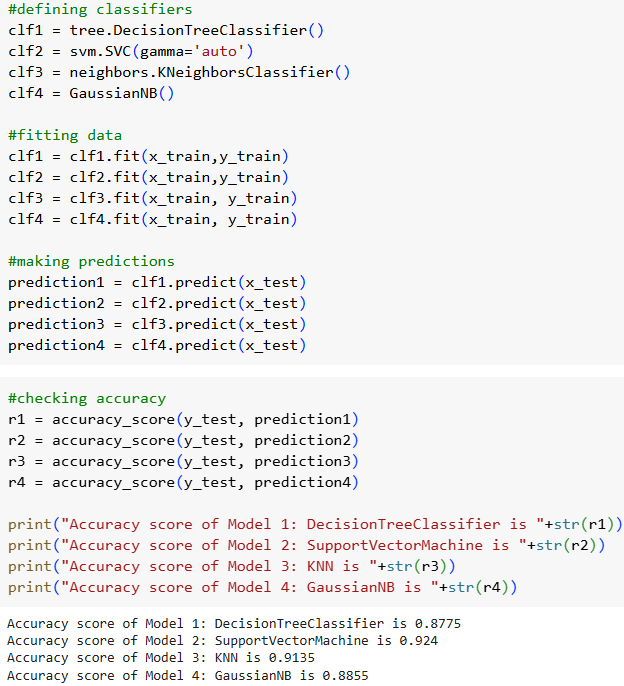
\includegraphics[width=0.8\linewidth]{graphics/dochinhxac.png}
    \caption{Độ chính xác của từng phân loại trên tập dữ liệu được chọn}
\end{figure}

\newpage

Nhìn chung, độ chính xác của phân loại Support Vector Machine cao nhất trong tất cả các phân loại (92,4\%)

Tiếp theo, cần phải có đánh giá về tỷ lệ phân loại sai của các mô hình phân loại:

\begin{figure} [!htp]
    \centering
    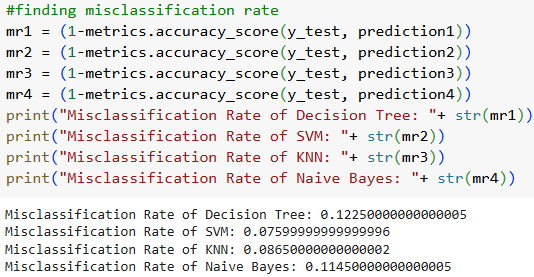
\includegraphics[width=0.75\linewidth]{graphics/sai.png}
    \caption{Tỷ lệ phân loại sai của từng mô hình phân loại trên tập dữ liệu được chọn}
\end{figure}

Vậy mô hình phân loại Support Vector Machine có tỷ lệ phân loại sai thấp nhất (7,6\%). Nên lựa chọn mô hình phân loại Support Vector Machine cho bài toán dự đoán giới tính là phù hợp nhất.

Lưu lại các tham số đã huấn luyện của mô hình trước đó và tiến hành chạy thử với dữ liệu giả định \textbf{chiều cao 166cm} và \textbf{cân nặng 77.7} kí ta thu được kết quả như sau:

\begin{figure}[!htp]
    \centering
    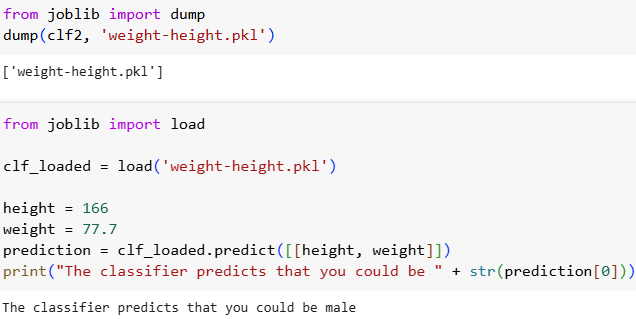
\includegraphics[width=0.75\linewidth]{graphics/ketqua_gender.png}
    \caption{Kết quả khi sử dụng mô hình SVM để dự đoán giới tính thông qua chiều cao và cân nặng}
\end{figure}

\subsubsection{Dự đoán tỷ lệ phần trăm mỡ của cơ thể}
Mặc dù trên ứng dụng Mi Fit có công thức tính toán tỷ lệ phần trăm mỡ của cơ thể, tuy nhiên sai số khi đo với cảm biến là rất lớn. Nhằm để giảm chi phí lắp đặt cảm biến lên cân cũng như giảm diện tích của trạm cân sức khoẻ nên em sử dụng trí tuệ nhân tạo (AI) để dự đoán cân nặng của 1 người thông qua các thông số như: độ tuổi, giới tính, chiều cao, và cân nặng. Mô hình được huấn luyện trên tập dữ liệu gồm các thông số như: \textbf{age}, \textbf{gender}, \textbf{height\_cm}, \textbf{weight\_kg}, \textbf{body\_fat}, \textbf{diastolic}, \textbf{systolic}, \textbf{gripForce}, \textbf{sit and bend forward\_cm}, \textbf{sit-ups counts}, \textbf{broad jump\_cm}, và \textbf{class} và khoảng 13400 bảng ghi. Cụ thể thông tin về bộ dữ liệu như sau:

\begin{figure} [!htp]
    \centering
    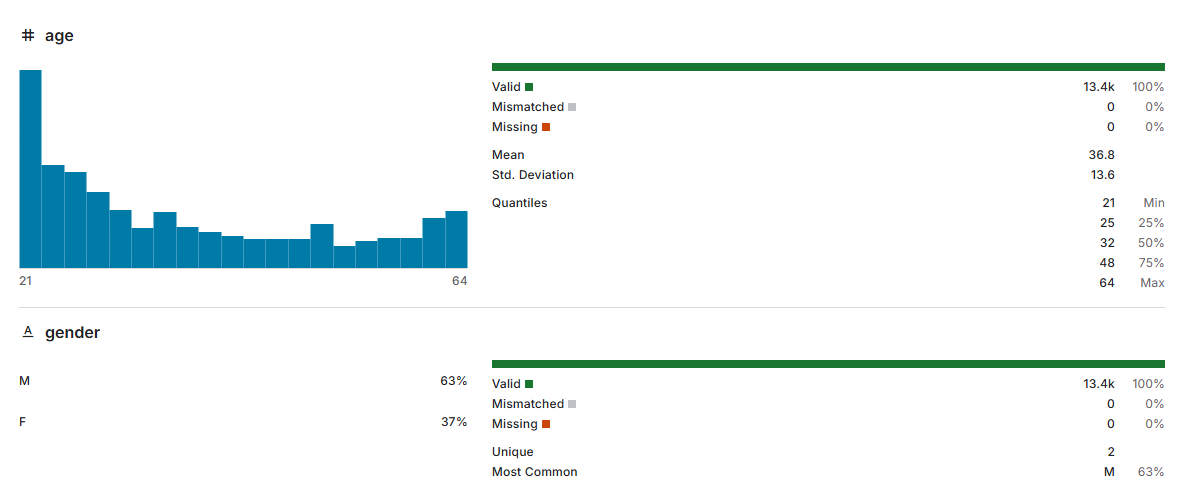
\includegraphics[width=1\linewidth]{graphics/BP_dataset_dotuoi_gioitinh.png}
    \caption{Thông tin độ tuổi và giới tính có trong bộ dữ liệu được huấn luyện để dự đoán tỷ lệ phần trăm mỡ trong cơ thể}
\end{figure}

\newpage

\begin{figure} [!htp]
    \centering
    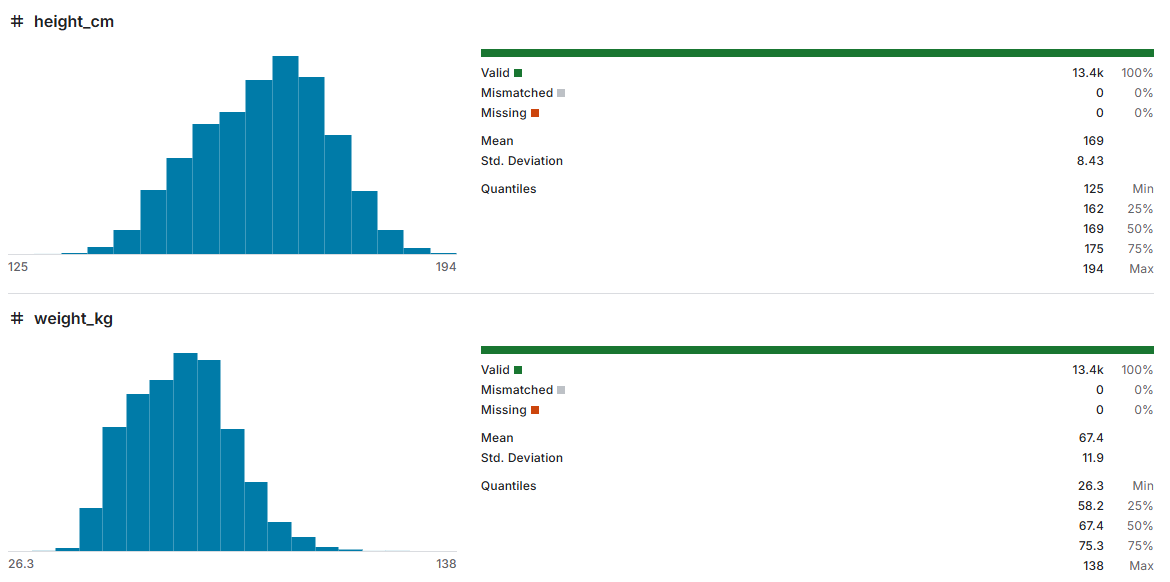
\includegraphics[width=1\linewidth]{graphics/BP_dataset_chieucao_cannang.png}
    \caption{Thông tin chiều cao và cân nặng có trong bộ dữ liệu được huấn luyện để dự đoán tỷ lệ phần trăm mỡ trong cơ thể}
\end{figure}

\begin{figure} [!htp]
    \centering
    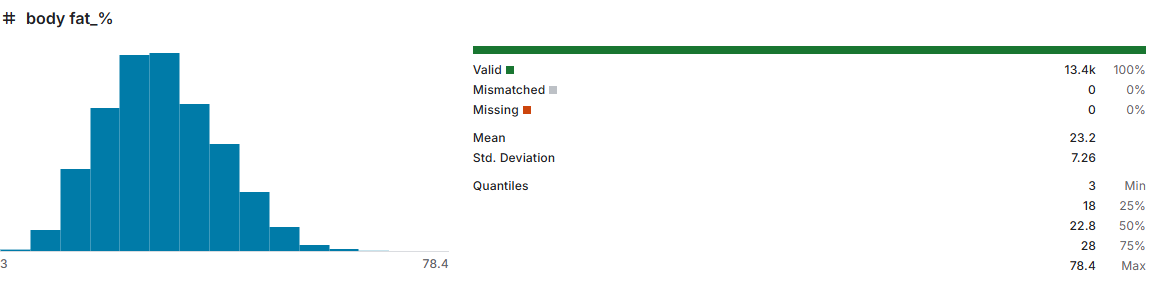
\includegraphics[width=1\linewidth]{graphics/BP_dataset_tylemo.png}
    \caption{Thông tin về tỷ lệ mỡ có trong bộ dữ liệu được huấn luyện để dự đoán tỷ lệ phần trăm mỡ trong cơ thể}
\end{figure}

Do bộ dữ liệu là dữ liệu liên tục (tuổi, chiều cao, cân nặng, tỷ lệ mỡ cơ thể). Hồi quy tuyến tính hoạt động tốt với các loại dữ liệu này, giúp xây dựng một đường thẳng để dự đoán giá trị liên tục của biến phụ thuộc dựa trên các biến độc lập. Nên chọn mô hình Hồi quy tuyến tính \textbf{(Linear Regression model)} là phù hợp để giải quyết bài toán dự đoán tỷ lệ mỡ của cơ thể. Sau khi sử dụng mô hình hồi quy tuyến tính trên bộ dữ liệu để dự đoán tỷ lệ mỡ em thu được các kết quả như sau:

\newpage

\begin{figure} [!htp]
    \centering
    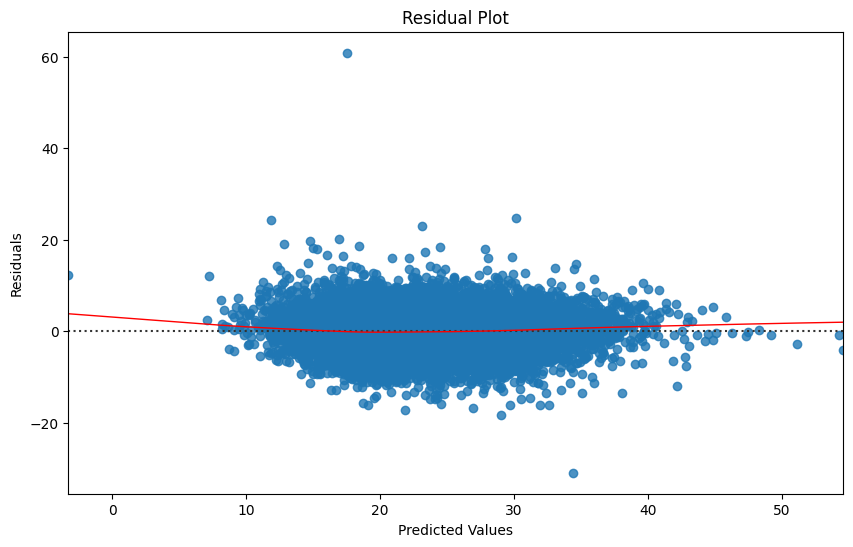
\includegraphics[width=0.8\linewidth]{graphics/residual_plot.png}
    \caption{Biểu đồ phần dư}
\end{figure}

Biểu đồ phần dư được sử dụng để kiểm tra độ phù hợp của mô hình hồi quy. Trên trục hoành là các giá trị dự đoán, còn trục tung biểu diễn phần dư (sai số giữa giá trị thực tế và giá trị dự đoán).

Một phân bố ngẫu nhiên của phần dư xung quanh trục 0 cho thấy mô hình phù hợp với dữ liệu và các giả định về tuyến tính và phương sai không đổi của sai số được đáp ứng.

Trong biểu đồ này, phần dư không có xu hướng rõ ràng theo bất kỳ hướng nào, tuy nhiên, có một số điểm ngoại lệ rõ rệt ở phía trên và dưới. Điều này cho thấy rằng, nhìn chung, mô hình có thể phù hợp, nhưng có thể cần xem xét lại các ngoại lệ đó để cải thiện chất lượng dự đoán hoặc xác minh các giả định.

\newpage

\begin{figure} [!htp]
    \centering
    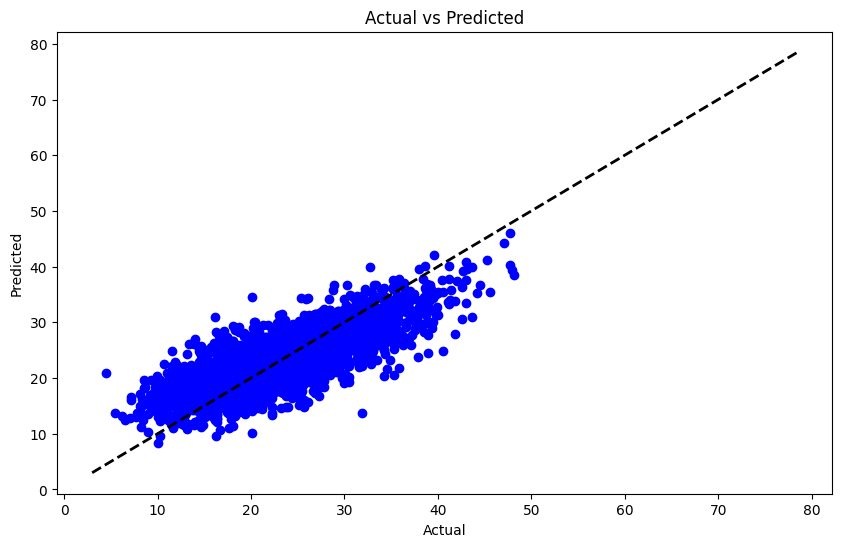
\includegraphics[width=0.8\linewidth]{graphics/ac_vs_pre.png}
    \caption{Biểu đồ phân tán}
\end{figure}

\textbf{Mối quan hệ tuyến tính:} Các điểm dữ liệu có xu hướng phân bố theo một đường thẳng, cho thấy có mối quan hệ tuyến tính giữa giá trị dự đoán và giá trị thực tế.

\textbf{Độ chính xác:} Phần lớn các điểm dữ liệu nằm gần đường thẳng y=x, cho thấy mô hình dự đoán khá chính xác. Tuy nhiên, vẫn có một số điểm dữ liệu nằm xa đường thẳng này, đặc biệt ở vùng giá trị lớn hơn 60.

\textbf{Các điểm ngoại lệ:} Có một số điểm dữ liệu nằm khá xa các điểm khác, đặc biệt ở vùng giá trị lớn hơn 60.

Biểu đồ phân tán này cho thấy mô hình dự đoán đã xây dựng được một mối quan hệ tuyến tính khá tốt giữa các biến độc lập và biến phụ thuộc.

\newpage

\begin{figure} [!htp]
    \centering
    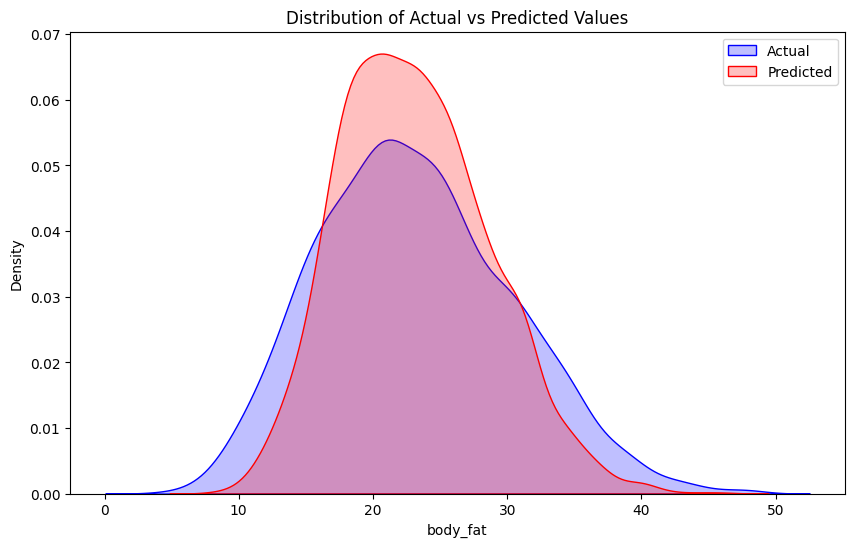
\includegraphics[width=0.8\linewidth]{graphics/dis_ac_vs_pre.png}
    \caption{Biểu đồ phân bố mật độ}
\end{figure}

\textbf{Phân phối tương đối giống nhau:} Cả hai đường cong của giá trị thực tế và dự đoán đều có hình dạng tương tự nhau, cho thấy mô hình đã bắt được xu hướng chung của dữ liệu.

\textbf{Mô hình có xu hướng dự đoán hơi thấp:} Đỉnh của đường cong dự đoán có vẻ hơi dịch chuyển về phía bên trái so với đỉnh của đường cong thực tế, cho thấy mô hình có xu hướng dự đoán giá trị phần trăm mỡ cơ thể hơi thấp so với giá trị thực tế.

Dựa trên biểu đồ này, có thể kết luận rằng mô hình hồi quy tuyến tính đã thực hiện khá tốt trong việc dự đoán lượng mỡ cơ thể. Tuy nhiên, vẫn còn một số không chính xác nhất định, đặc biệt là mô hình có xu hướng đánh giá thấp lượng mỡ cơ thể.

\newpage

\begin{figure} [!htp]
    \centering
    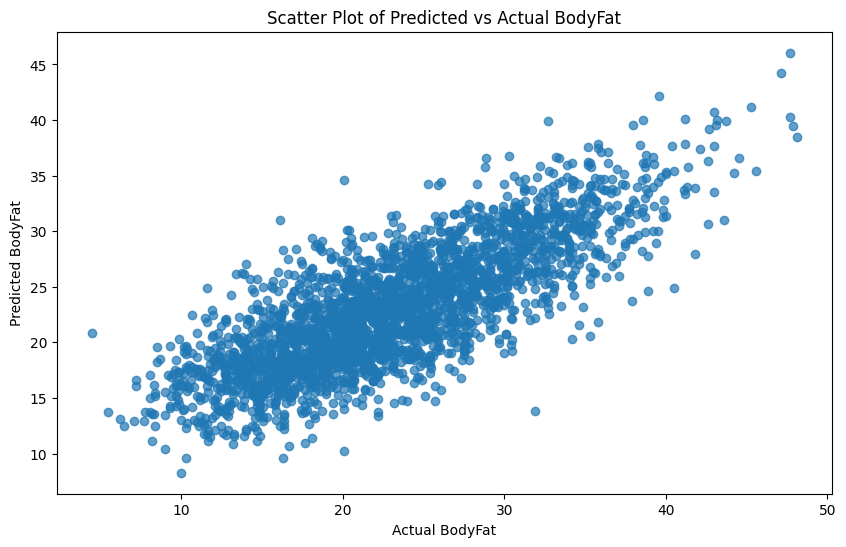
\includegraphics[width=0.8\linewidth]{graphics/scatt_pre_vs_ac.png}
    \caption{Biểu đồ phân tán}
\end{figure}

\textbf{Mối quan hệ tuyến tính:} Các điểm dữ liệu có xu hướng phân bố theo một đường thẳng, cho thấy có mối quan hệ tuyến tính giữa giá trị dự đoán và giá trị thực tế.

\textbf{Độ chính xác:} Phần lớn các điểm dữ liệu nằm gần đường thẳng y=x, cho thấy mô hình dự đoán khá chính xác. Tuy nhiên, vẫn có một số điểm dữ liệu nằm xa đường thẳng này, đặc biệt ở vùng giá trị thực tế lớn hơn 40.

\textbf{Các điểm ngoại lệ:} Có một số điểm dữ liệu nằm khá xa các điểm khác, đặc biệt ở vùng giá trị thực tế nhỏ hơn 15 và lớn hơn 45.

Biểu đồ phân tán này cho thấy mô hình hồi quy tuyến tính đã xây dựng được một mối quan hệ tuyến tính khá tốt giữa các biến độc lập và biến phụ thuộc.

Từ những đánh giá sơ bộ trên có thể kết luận rằng mô hình Linear Regression phù hợp với bài toán dự đoán tỷ lệ mỡ trên cơ thể. Thử nghiệm mô hình trên giá trị giả định: \textbf{25 tuổi}, \textbf{giới tính nam}, \textbf{chiều cao 166 cm}, và \textbf{cân nặng 77.7 kí} cho kết quả như sau:

\newpage

\begin{figure} [!htp]
    \centering
    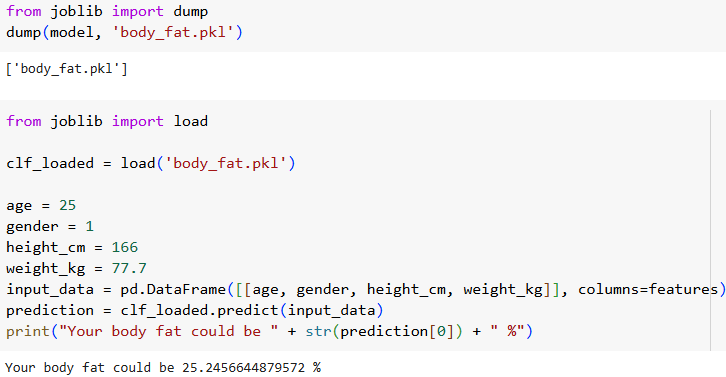
\includegraphics[width=0.9\linewidth]{graphics/result_bf.png}
    \caption{Kết quả dự đoán phần trăm mỡ dựa trên dữ liệu đầu vào giả định}
\end{figure}

\subsubsection{Đo độ thăng bằng của cơ thể}

Chức năng này sử dụng MediaPipe và OpenCV để theo dõi tư thế người dùng qua camera, thu thập mẫu chuẩn và đo độ thăng bằng dựa trên vị trí tâm khối (COM).

\newpage
\begin{figure}[!htp]
    \centering
    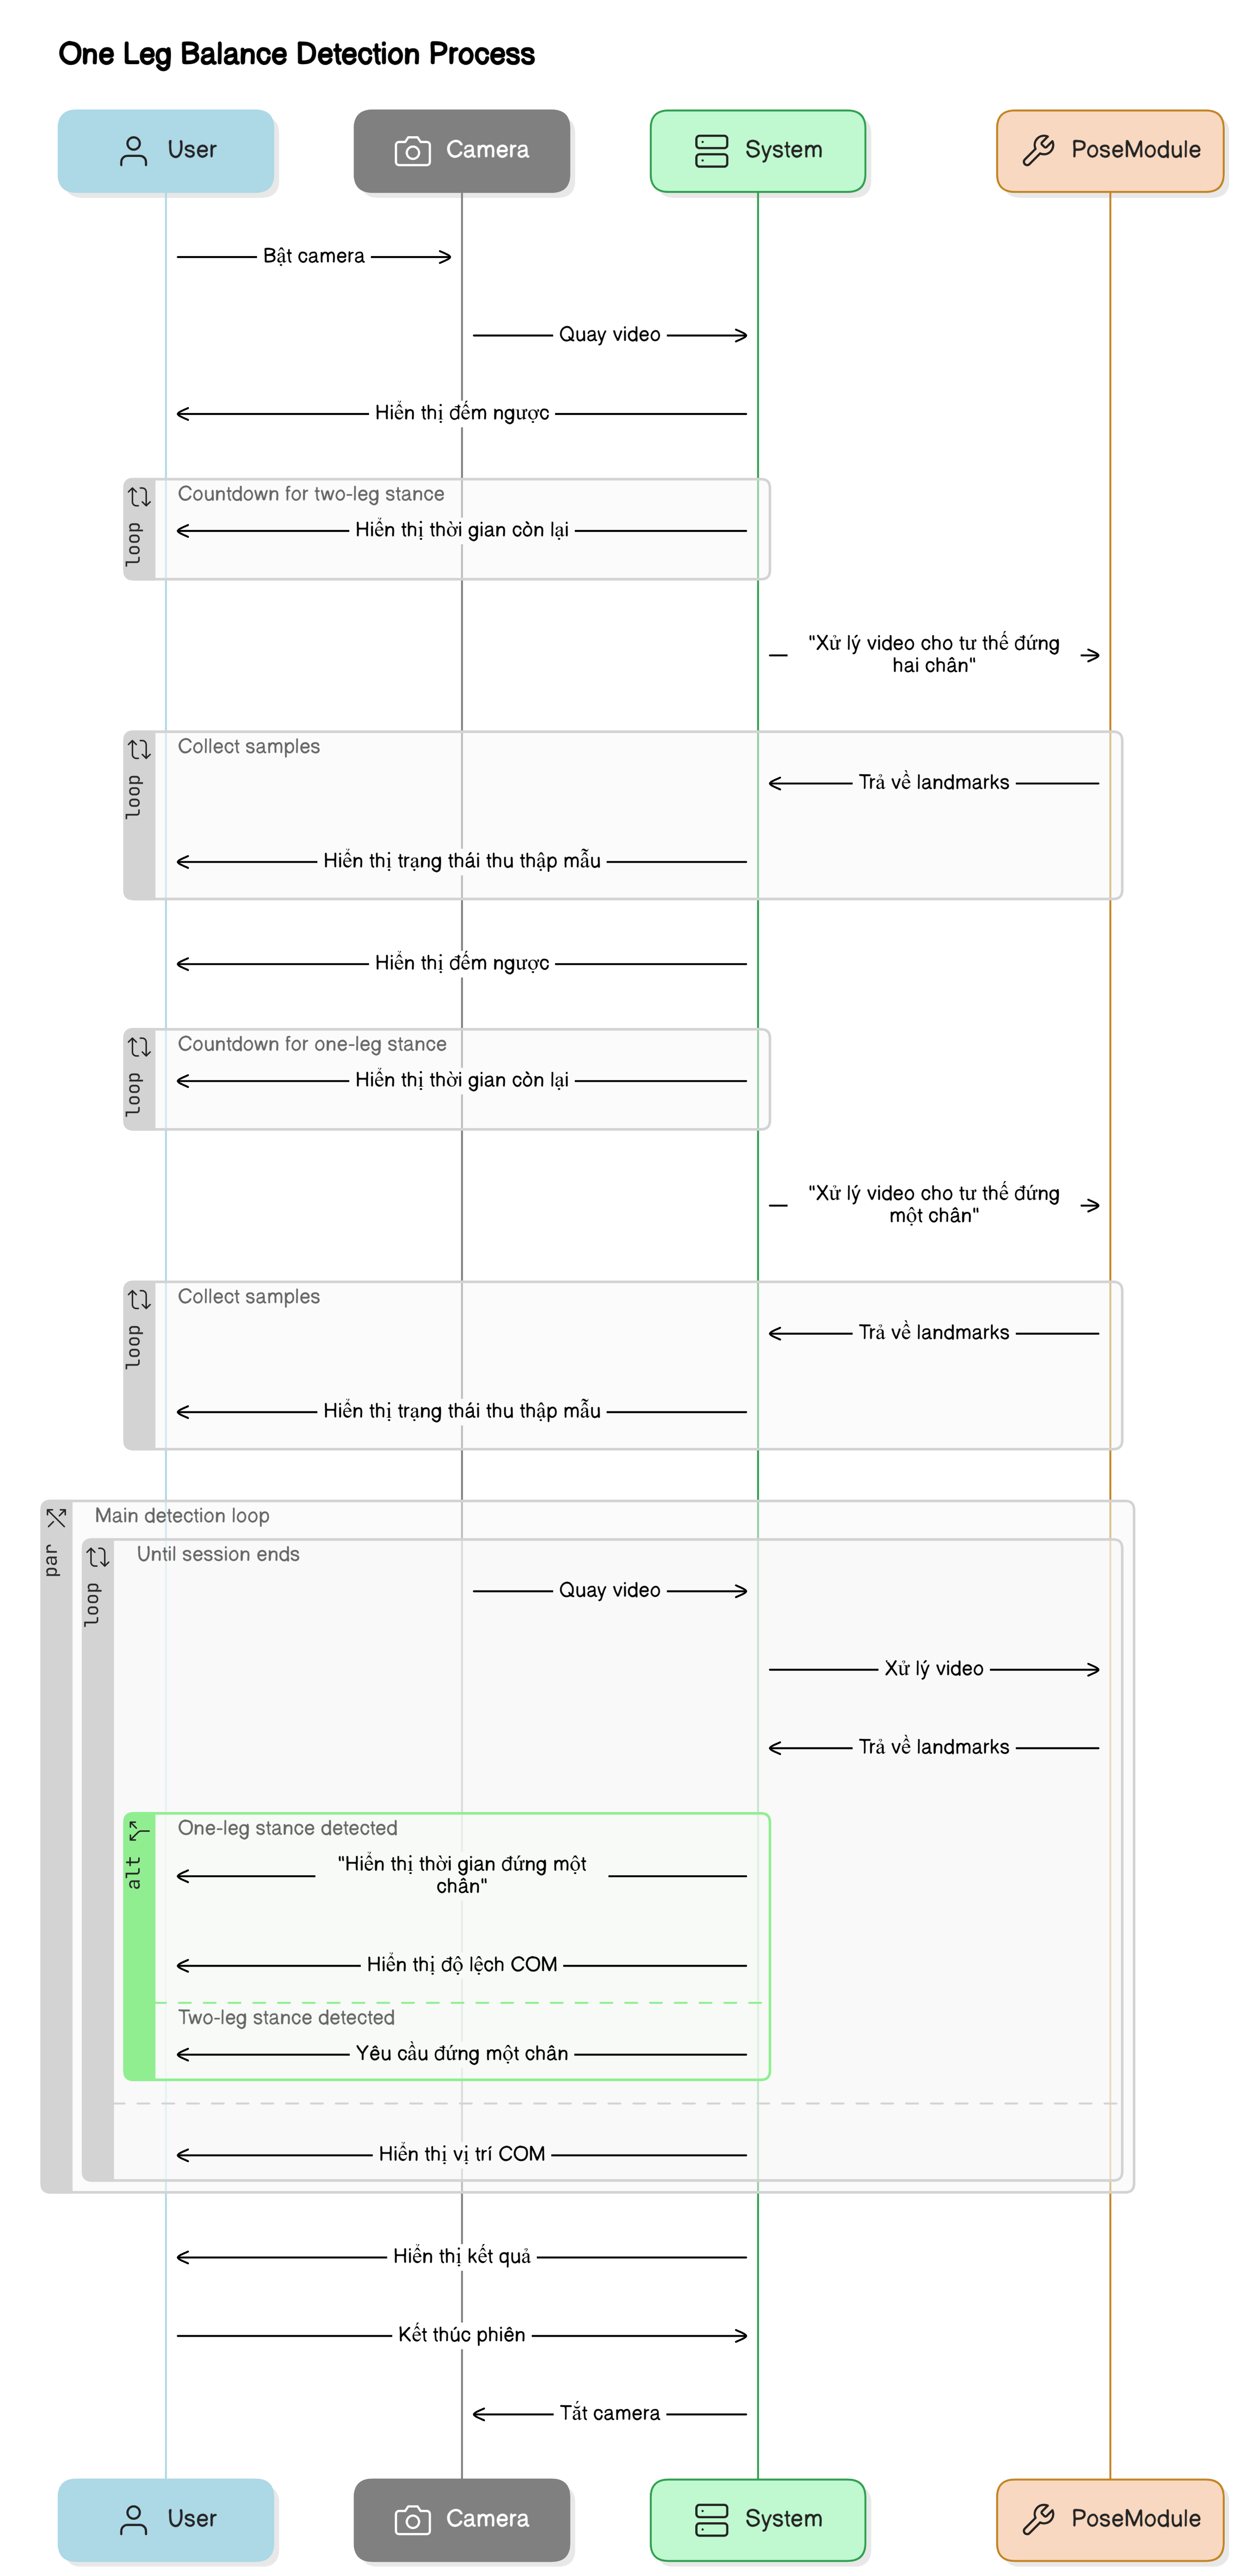
\includegraphics[width=0.6\linewidth]{graphics/oneleg_chart.png}
    \caption{Quá trình nhận diện thời gian thăng bằng 1 chân}
\end{figure}
\newpage

\paragraph{Kiến trúc và luồng hoạt động}
\begin{itemize}
  \item \textbf{Giai đoạn thu thập mẫu chuẩn:} Người dùng đứng hai chân để thu thập mẫu \texttt{two\_legs\_samples}, sau đó đứng một chân để thu thập mẫu \texttt{one\_leg\_samples}. Mỗi mẫu là một vector tọa độ landmarks.
  \item \textbf{Giai đoạn đo đạc chính:} Xử lý video liên tục, xác định tư thế hiện tại qua cosine similarity giữa vector hiện tại và hai bộ mẫu. Khi phát hiện tư thế một chân, ghi nhận thời gian và độ lệch COM.
  \item \textbf{Giai đoạn kết thúc:} Khi người dùng trở về tư thế hai chân, tính tổng thời gian đứng một chân và độ lệch trung bình, trả về kết quả.
\end{itemize}

\paragraph{Phân tích chi tiết các thành phần}

\subparagraph{Xử lý video và hiển thị}
\begin{itemize}
  \item Sử dụng \texttt{cv2.VideoCapture} để lấy khung hình, \texttt{cv2.putText}, \texttt{cv2.circle}, \texttt{cv2.imshow} để vẽ hướng dẫn và kết quả.
  \item Hàm \texttt{countdown(cap, duration, message)}: vòng lặp dựa trên \texttt{time.time()}, cập nhật thời gian còn lại và hiển thị đếm ngược, cho phép thoát sớm bằng phím \texttt{q}.
\end{itemize}

\subparagraph{Trích xuất và chuyển đổi landmarks}
\begin{itemize}
  \item Khởi tạo \texttt{mp\_pose.Pose} với \texttt{min\_detection\_confidence=0.5} và \texttt{min\_tracking\_confidence=0.5}.
  \item \texttt{landmarks\_to\_vector(landmarks)}: chuyển danh sách landmarks thành vector NumPy 1 chiều chứa \texttt{[x\_1, y\_1, x\_2, y\_2, \dots]}.
\end{itemize}

\subparagraph{Đo độ tương đồng giữa các mẫu}
\begin{itemize}
  \item \texttt{calculate\_max\_similarity(current\_vector, samples)}: lặp qua các mẫu, tính cosine similarity bằng \texttt{1 - cosine(v1, v2)}, chọn giá trị cao nhất để quyết định tư thế.
\end{itemize}

\subparagraph{Thu thập mẫu}
\begin{itemize}
  \item \texttt{collect\_samples(pose, cap, num\_samples, instruction\_text)}: thu thập \texttt{num\_samples} vector landmarks trong tối đa 30 giây, chờ 1 giây giữa mỗi mẫu, hiển thị số lượng mẫu đã thu.
\end{itemize}

\subparagraph{Phân tích phiên “đứng một chân”}
\begin{itemize}
  \item \texttt{one\_leg\_balance\_detection(camera\_index, num\_samples)}:
    \begin{enumerate}
      \item Đếm ngược chuẩn bị, thu hai bộ mẫu (hai chân và một chân).
      \item Với mỗi khung hình, ước tính COM qua trung điểm hông trái – hông phải, quy đổi sang pixel.
      \item Tính cosine similarity với hai bộ mẫu, xác định tư thế.
      \item Khi ở tư thế một chân, bắt đầu phiên, tính offset theo trục \(x\) giữa COM hiện tại và COM baseline, lưu vào \texttt{session\_offsets}.
      \item Khi quay về hai chân, kết thúc phiên, tính \(\text{session\_duration}\) và \(\text{avg\_offset}\), trả về kết quả.
    \end{enumerate}
\end{itemize}

\paragraph{Ưu điểm và hướng cải thiện}

\subparagraph{Ưu điểm}
\begin{itemize}
  \item Giao diện trực quan: đếm ngược, hướng dẫn và kết quả thời gian thực.
  \item Sử dụng cosine similarity hiệu quả để phân loại tư thế.
  \item Quy trình rõ ràng, dễ bảo trì.
\end{itemize}

\subparagraph{Hạn chế và cải thiện}
\begin{itemize}
  \item Ứng dụng COM chỉ dựa trên trung điểm hông có thể thiếu chính xác; có thể bổ sung các điểm khác như vai, đầu gối.
  \item Cần xử lý nhiễu từ landmarks (ánh sáng, góc quay) bằng bộ lọc hoặc smoothing.
  \item Thay vì \texttt{time.sleep(1)}, có thể sampling linh hoạt dựa trên thay đổi thực tế của landmarks.
\end{itemize}

\paragraph{Kết luận}

Giải pháp cho phép đo độ thăng bằng dựa trên phân tích COM từ MediaPipe, với quy trình thu thập mẫu và đo đạc rõ ràng. Tuy còn một số hạn chế về độ chính xác và hiệu suất, khung sườn hiện tại là nền tảng vững chắc cho các cải tiến sau này.


\subsubsection{Đưa ra các đánh giá và lời khuyên dựa trên các chỉ số của cơ thể}
Sau khi nội suy và dự đoán các thông số sức khoẻ của cơ thể, sử dụng \href{https://aistudio.google.com/u/0/apikey}{API của mô hình Google Gemini Pro 1.5 Flash} để đưa ra các đánh giá và lời khuyên để cải thiện sức khoẻ người dùng.

\begin{figure} [!htp]
    \centering
    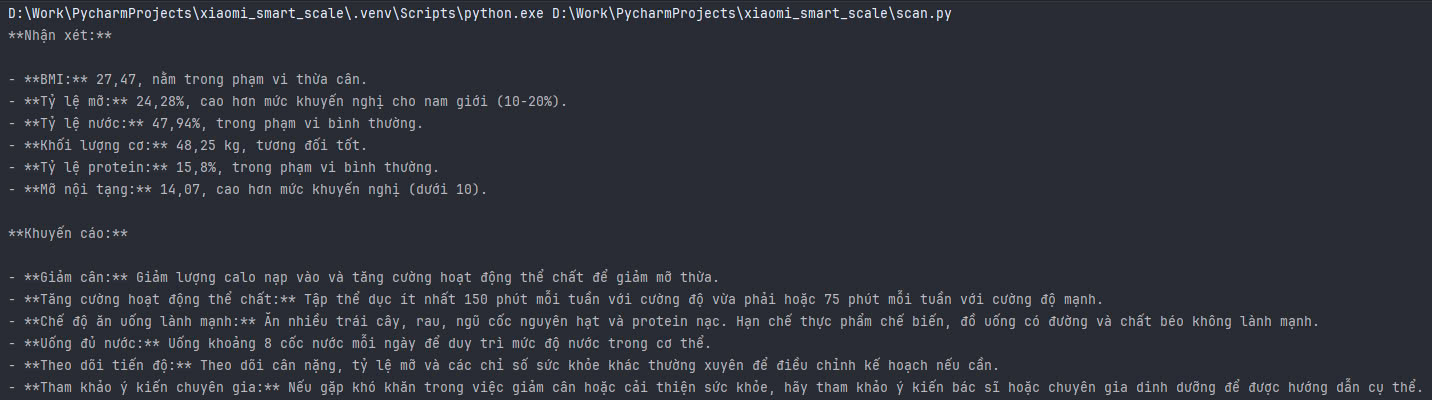
\includegraphics[width=1\linewidth]{graphics/ai_rcmd.jpg}
    \caption{Sử dụng AI để đánh giá và đưa ra các lời khuyên về sức khoẻ của người dùng}
\end{figure}

\subsubsection{Đọc các đánh giá và lời khuyên cho người dùng}
Sau nhận các đánh giá từ AI, sử dụng \href{https://pypi.org/project/gTTS/}{thư viện gTTS (Google Text-to-Speech)} để đọc các đánh giá cho người dùng

\begin{lstlisting}[language=python,caption={Sử dụng thư viện gTTS để đọc các đánh giá của AI}]
from gtts import gTTS
import os

def read_recommend_vietnamese(user_info, text):

    tts = gTTS(text = text, lang = 'vi', slow=False)

    tts.save("audio/audio.mp3")

    os.system("start audio/audio.mp3")  # Windows
\end{lstlisting}

\subsection{Đánh giá các số liệu nội suy và dự đoán bởi AI so với thiết bị có cảm biến}
Để đánh giá các chỉ số cơ thể từ nội suy theo công thức và dự đoán bằng trí tuệ nhân tạo, em sử dụng cân điện tử \textbf{Xiaomi Smart Scale 2} để lấy cân nặng ban đầu và tiến hành tính toán, dự đoán ra các thông số cơ thể so sánh với thiết bị cân điện tử có cảm biến \textbf{(Xiaomi Scale Composition S400)} thu được bảng sau:

\begin{table}[!htp]
\centering
\begin{tabular}{clccr}
\toprule
STT & Chỉ số & Xiaomi Smart Scale 2 & Xiaomi Scale Composition S400 & Sai số \\
\midrule
1 & Cân nặng & 75.55 & 75.6 & 0.07\% \\
2 & BMI & 27.42 & 27.4 & 0.07\% \\
3 & BMR & 1755.21 & 1599 & 9.77\% \\
4 & TDEE & 2720.58 & None &  None\\
5 & LBM & 51.58 & 56.8 & 9.19\% \\
6 & Phần trăm mỡ (AI) & 24.21 & 24.8 & 2.38\% \\
8 & Phần trăm nước & 47.99 & 52.5 & 8.59\% \\
9 & Khối lượng xương & 2.58 & 2.9 & 11.03\% \\
10 & Khối lượng cơ & 48.2 & 53.9 & 10.58\% \\
11 & Phần trăm protein & 15.81 & 18 & 12.17\% \\
12 & Mỡ nội tạng & 14 & 10 & 40.00\% \\
13 & Cân nặng lý tưởng & 60.2 & 60.2 & 0.00\% \\
\bottomrule
\end{tabular}
\caption{So sánh chỉ số giữa các thông số tính toán và Xiaomi Scale Composition S400}
\end{table}

Bảng so sánh trên cung cấp một cái nhìn chi tiết về sự khác biệt giữa các thông số nội suy theo công thức, dự đoán bằng AI và Xiaomi Scale Composition S400. Cả hai đều thể hiện được các chỉ số cơ thể cơ bản như cân nặng, BMI, nhưng S400 cung cấp nhiều thông tin chi tiết hơn về thành phần cơ thể.

Nhìn chung, các chỉ số đo được từ S400 có sự chênh lệch không đáng kể so với các thông số nội suy và dự đoán, ngoại trừ một số chỉ số như mỡ nội tạng có sự chênh lệch khá lớn (40\%).

Tuy nhiên, có một số lưu ý như:

\begin{itemize}
    \item \textbf{Sai số:} Mặc dù S400 cho kết quả chi tiết hơn, nhưng vẫn tồn tại sai số nhất định ở một số chỉ số. Do đó, không nên quá phụ thuộc vào một lần đo mà nên theo dõi kết quả trong một thời gian dài để có cái nhìn tổng quan chính xác hơn.
    \item \textbf{Giá thành:} Thông thường, các mẫu cân có nhiều tính năng hơn sẽ có giá thành cao hơn. Vì vậy, S400 có thể có giá thành cao hơn so với một chiếc cân điện tử thông thường được áp dụng các công thức nội suy và dự đoán của AI.
\end{itemize}

\subsection{Lưu trữ thông tin người dùng}
Những thông tin cơ bản của người dùng và các chỉ số đo, tính toán được sẽ được lưu lại dưới dạng 1 file .csv để có thể trực quan hoá và phục vụ cho mục đích nghiên cứu sau này, file .csv lưu lại các thông tin sau: \textbf{datetime, name, age, gender, height, weight, dob, activity\_factor, bmi, bmr, tdee, lean\_body\_mass, fat\_percentage, water\_percentage, bone\_mass, muscle\_mass, protein\_percentage, visceral\_fat, ideal\_weight}

\begin{figure}[!htp]
    \centering
    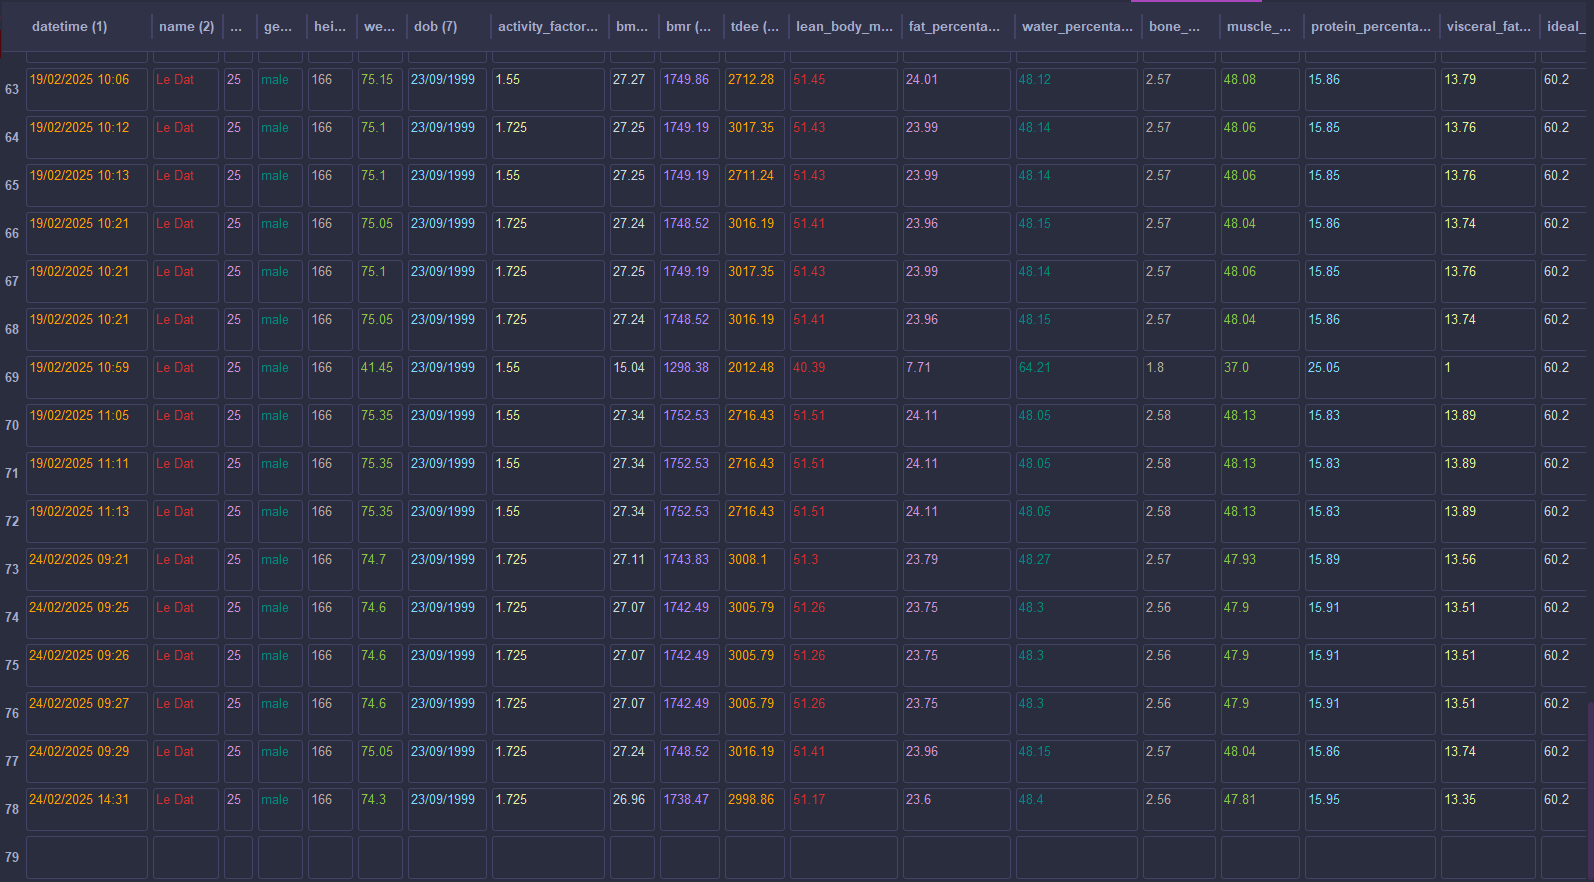
\includegraphics[width=0.7\linewidth]{graphics/csv.png}
    \caption{Các thông tin của người dùng được lưu trữ trong file csv}
\end{figure}

\subsection{Trực quan hóa dữ liệu sức khỏe thông qua CoreIoT}
\subsubsection{Cấu hình thiết bị trên nền tảng IoT}
Trên nền tảng CoreIoT, việc cấu hình thiết bị là bước quan trọng nhằm trực quan hóa các thông số sức khỏe, cho phép Gateway giao tiếp hiệu quả với nền tảng thông qua giao thức MQTT. Để thực hiện, người dùng cần truy cập vào thẻ \textbf{Entities}, sau đó chọn thẻ con \textbf{Devices} để thiết lập kết nối và truyền dữ liệu từ thiết bị IoT.

\begin{figure}[!htp]
    \centering
    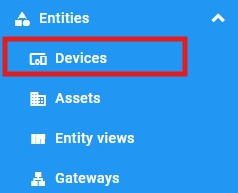
\includegraphics[width=0.5\linewidth]{graphics/coreiot_device.png}
    \caption{Chọn thẻ Devices để cấu hình thiết bị giao tiếp với nền tảng CoreIoT}
    \label{fig:coreiot-device}
\end{figure}
\newpage

Trong phần \textbf{Device Credentials}, người dùng cần thiết lập phương thức xác thực cho thiết bị. Nền tảng CoreIoT hỗ trợ nhiều tùy chọn xác thực, bao gồm \textbf{Access token}, \textbf{X.509}, và \textbf{MQTT Basic}. Trong dự án này, phương thức \textbf{MQTT Basic} được sử dụng, tận dụng các thông tin như \textbf{ClientID}, \textbf{User Name}, và \textbf{Password} để đảm bảo thiết bị kết nối an toàn và ổn định với nền tảng.

\begin{figure}[!htp]
    \centering
    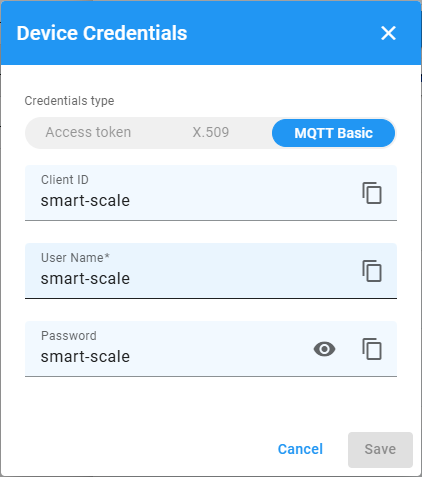
\includegraphics[width=0.5\linewidth]{graphics/coreiot_mqtt.png}
    \caption{Cấu hình Device Credentials trên nền tảng CoreIoT}
    \label{fig:device-credentials}
\end{figure}

Sau khi hoàn tất việc thiết lập thông tin xác thực trong thẻ \textbf{Device Credentials}, các thông tin này sẽ được sử dụng để cấu hình trong mã nguồn của thiết bị. Quy trình này đảm bảo thiết bị giao tiếp chính xác với nền tảng CoreIoT.

\begin{figure}[!htp]
    \centering
    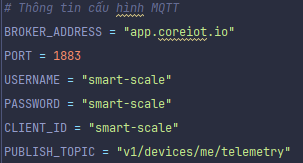
\includegraphics[width=0.5\linewidth]{graphics/mqtt_info.png}
    \caption{Cấu hình các thông số xác thực MQTT trong mã nguồn của thiết bị}
    \label{fig:mqtt-config}
\end{figure}

Để truyền các giá trị thông số sức khỏe từ thiết bị lên nền tảng CoreIoT, đoạn mã sau được sử dụng:

\begin{lstlisting}[language=python,caption={Gửi dữ liệu sức khỏe lên CoreIoT qua MQTT}]
mqtt_client.publish(PUBLISH_TOPIC, health_data.get_body_composition())
\end{lstlisting}

Trong đó, \textbf{PUBLISH\_TOPIC = "v1/devices/me/telemetry"} là topic mặc định mà nền tảng CoreIoT sử dụng để nhận dữ liệu từ thiết bị.

Cuối cùng, để kiểm tra và quan sát các giá trị thông số sức khỏe đã được cập nhật, người dùng có thể chuyển sang thẻ \textbf{Latest telemetry} của thiết bị trên giao diện CoreIoT.

\begin{figure}[!htp]
    \centering
    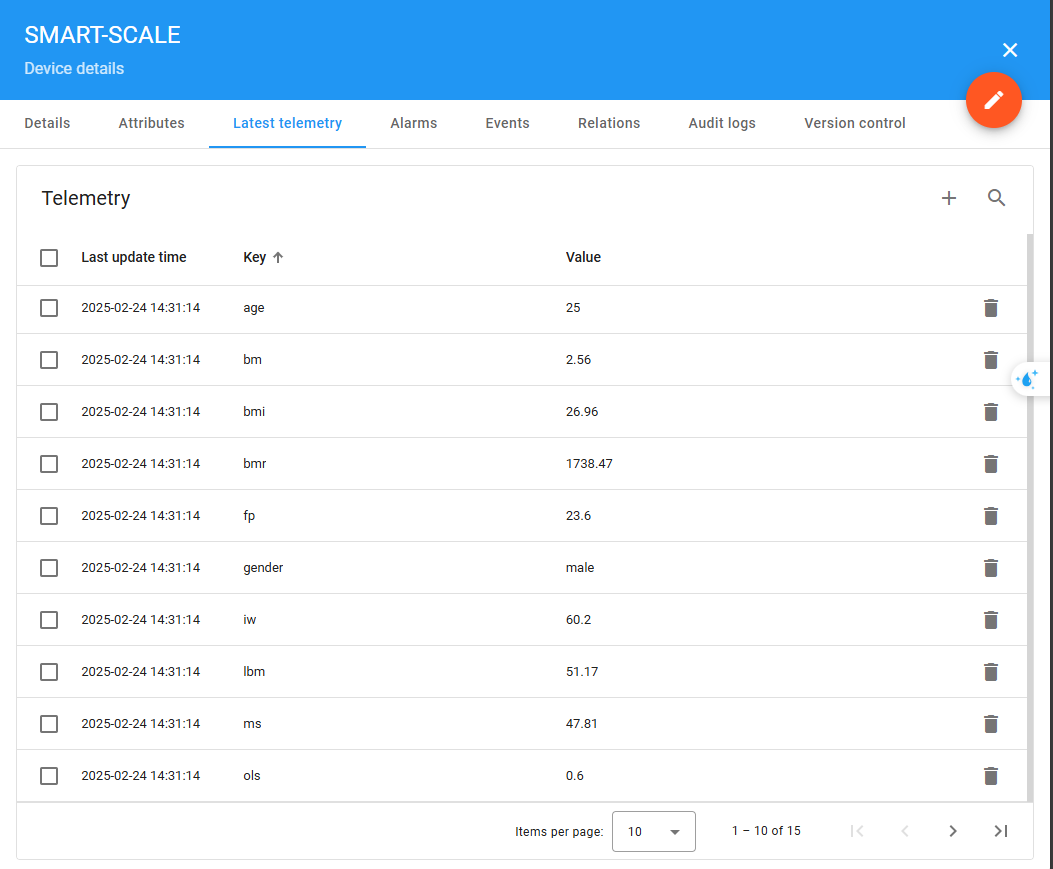
\includegraphics[width=0.8\linewidth]{graphics/lastest_telemetry.png}
    \caption{Các giá trị thông số sức khỏe được cập nhật trong thẻ Latest telemetry của thiết bị}
    \label{fig:latest-telemetry}
\end{figure}

\newpage

\subsubsection{Cài đặt bảng điều khiển để hiển thị các thông số sức khỏe}

Sau khi các thông số sức khỏe từ cân điện tử thông minh đã được truyền tải và hiển thị trong thẻ \textbf{Latest telemetry} của thiết bị trên giao diện CoreIoT, bước tiếp theo là chuyển sang thẻ \textbf{Dashboard} để cấu hình và trực quan hóa các thông số này trên bảng điều khiển chính.

\begin{figure}[!htp]
    \centering
    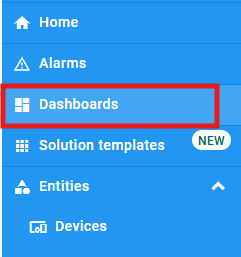
\includegraphics[width=0.5\linewidth]{graphics/dashboard.png}
    \caption{Thẻ Dashboard trên giao diện của nền tảng CoreIoT}
    \label{fig:dashboard-tab}
\end{figure}

\newpage

Tiếp theo, người dùng cần tạo một Dashboard mới và đặt tên cho nó để dễ dàng quản lý và nhận diện.

\begin{figure}[!htp]
    \centering
    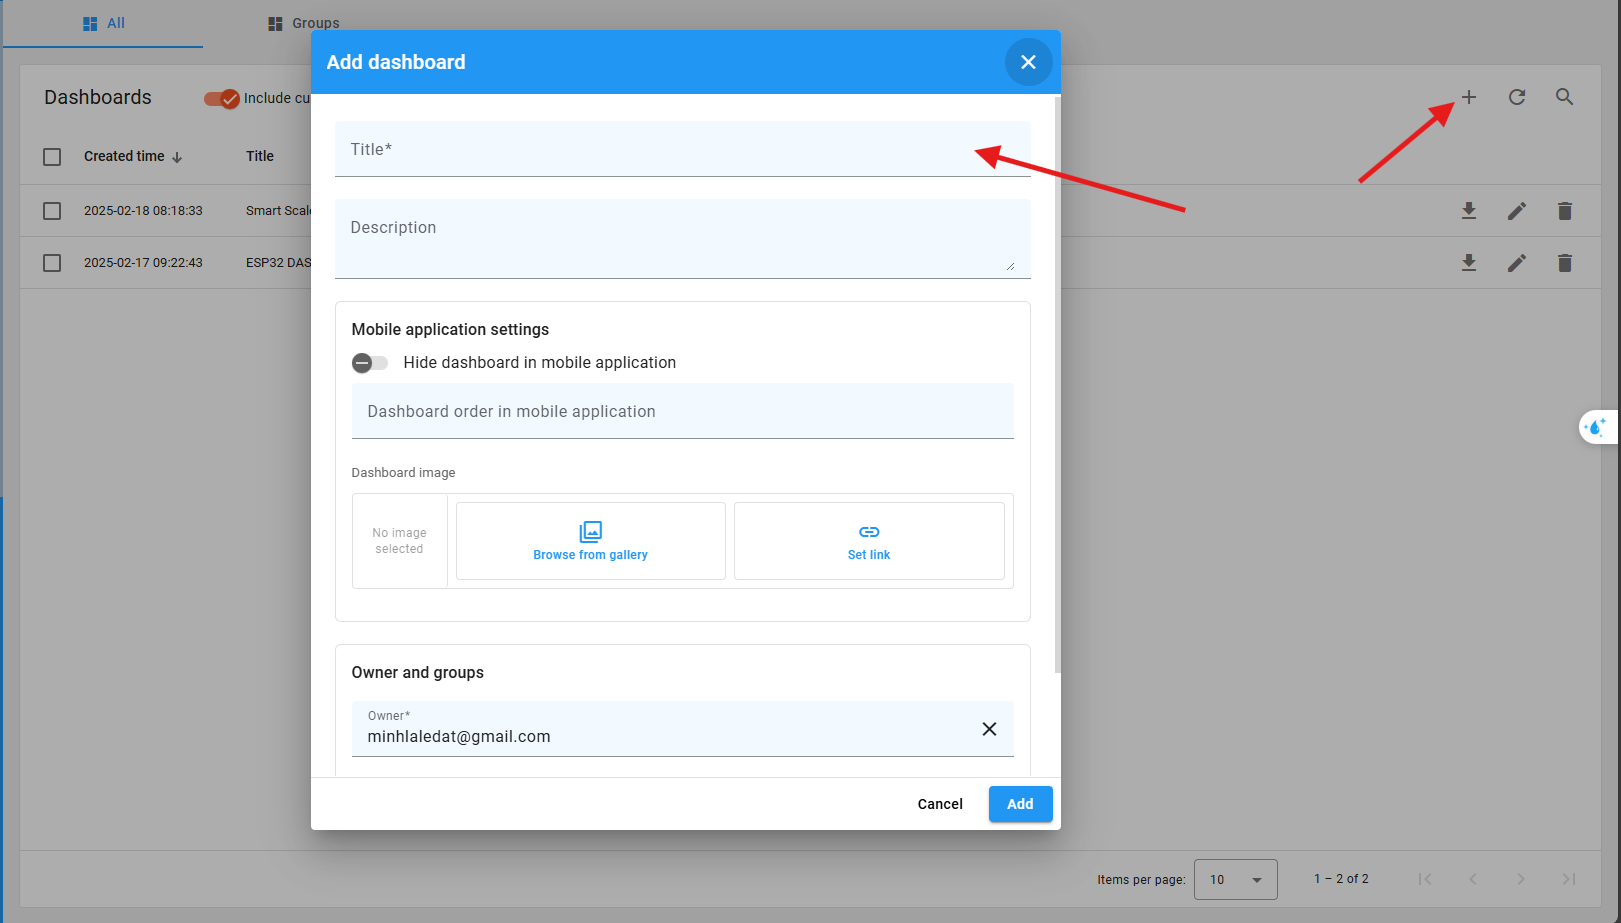
\includegraphics[width=0.9\linewidth]{graphics/create_named_dashboard.png}
    \caption{Tạo và đặt tên cho Dashboard mới}
    \label{fig:create-dashboard}
\end{figure}

Sau khi Dashboard được tạo, người dùng có thể thêm các phần tử (widgets) để hiển thị trực quan các thông số sức khỏe, giúp theo dõi dữ liệu một cách hiệu quả.

\begin{figure}[!htp]
    \centering
    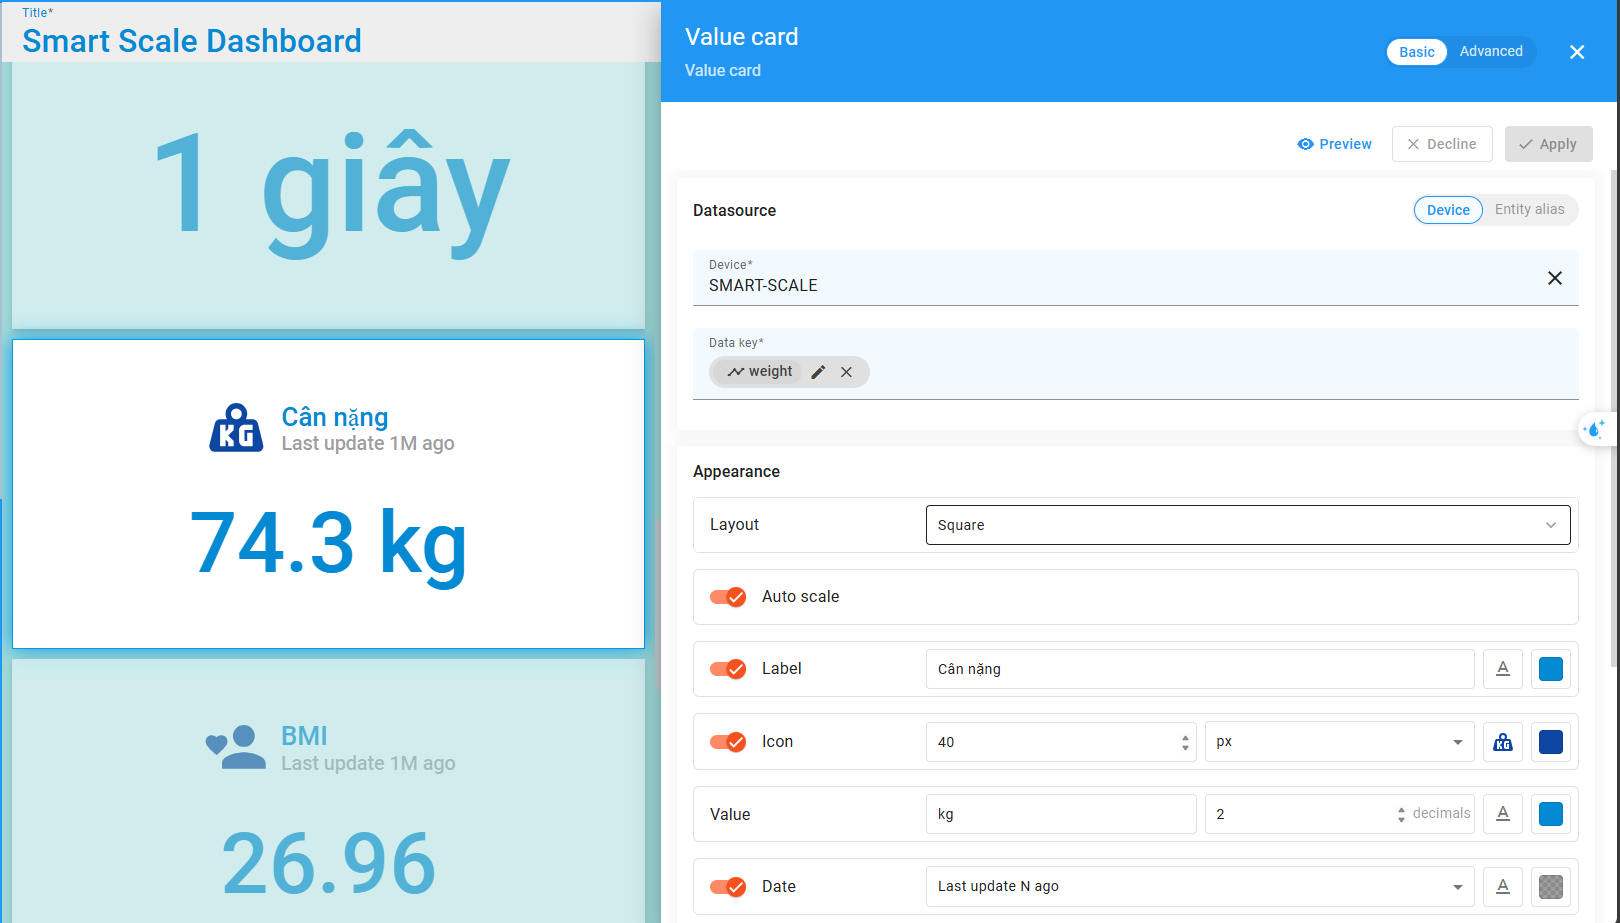
\includegraphics[width=0.75\linewidth]{graphics/init_element_dashboard.png}
    \caption{Cấu hình các thông số cho phần tử hiển thị trên Dashboard}
    \label{fig:config-widget}
\end{figure}

\newpage

Trong quá trình cấu hình phần tử, người dùng cần cung cấp các thông tin sau:

\begin{itemize}
    \item \textbf{Device:} Tên của thiết bị đã được thiết lập trước đó trong mục \textbf{Entities} > \textbf{Devices}.
    \item \textbf{Data key:} Giá trị tương ứng với thông số sức khỏe được truyền từ Gateway, có thể tra cứu trong thẻ \textbf{Latest telemetry}.
\end{itemize}

Ngoài ra, nền tảng CoreIoT còn cung cấp các tùy chọn tinh chỉnh như màu sắc, kích thước và kiểu hiển thị của các phần tử trên Dashboard, cho phép người dùng điều chỉnh giao diện theo nhu cầu cụ thể.

\begin{figure}[!htp]
    \centering
    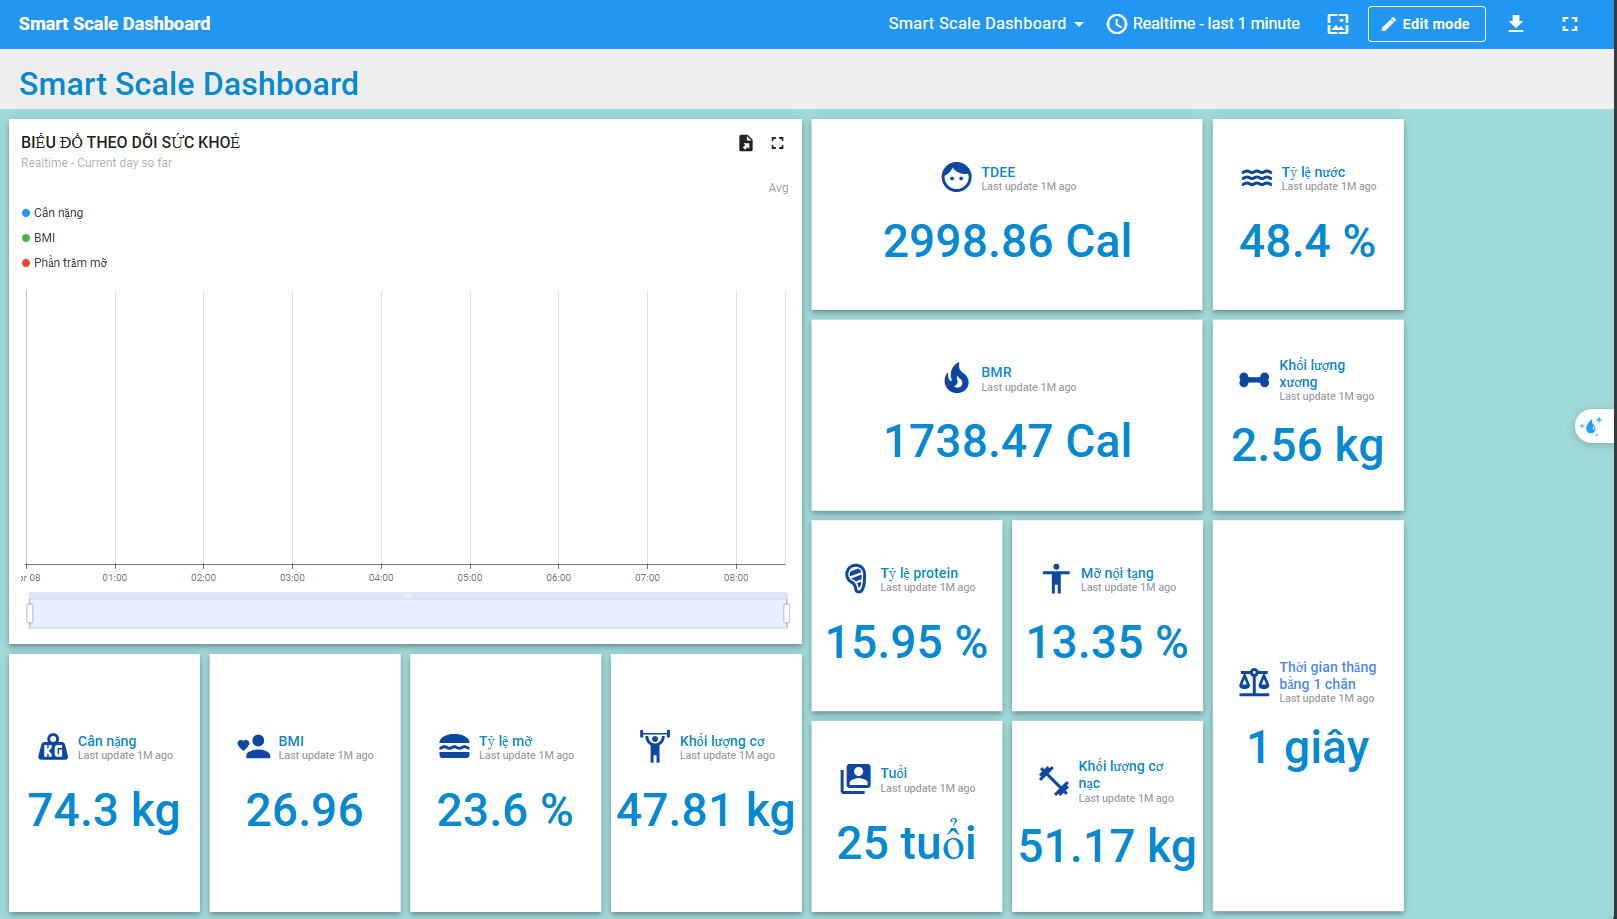
\includegraphics[width=0.75\linewidth]{graphics/final_dashboard.png}
    \caption{Dashboard của dự án sau khi được tinh chỉnh và hoàn thiện}
    \label{fig:final-dashboard}
\end{figure}
\section{TỔNG KẾT}

Trong bối cảnh chuyển đổi số ngày càng lan rộng và đóng vai trò then chốt trong lĩnh vực y tế, đề tài \textbf{\textit{“Xây dựng hệ thống chăm sóc sức khỏe điện tử với thiết bị theo dõi sức khỏe thông minh”}} đã được triển khai với kỳ vọng góp phần đổi mới phương thức theo dõi và quản lý sức khỏe cá nhân, đồng thời hỗ trợ hiệu quả cho các cơ sở y tế trong công tác giám sát cộng đồng. Qua quá trình thực hiện, hệ thống đã tích hợp thành công giữa phần cứng (thiết bị cân thông minh) và phần mềm (nền tảng phân tích và hiển thị dữ liệu sức khỏe), tạo nên một giải pháp có tính ứng dụng cao và phù hợp với thực tiễn.

\subsection{Đánh giá kết quả thực hiện}

Về mặt kỹ thuật, hệ thống đã đạt được các yêu cầu đặt ra trong đề tài. Cụ thể:

\begin{itemize}
  \item \textbf{Khả năng thu thập và xử lý dữ liệu}: Hệ thống đã kết nối thành công với các thiết bị cân sức khỏe thông minh thông qua Bluetooth Low Energy, trích xuất chính xác các thông số như cân nặng, tỷ lệ mỡ, khối lượng cơ, nước, xương, v.v. Dữ liệu được lưu trữ có tổ chức và có thể tái sử dụng cho các mục đích phân tích sau này.
  
  \item \textbf{Phân tích và nội suy thông số sinh học}: Thông qua các công thức y sinh học và kỹ thuật nội suy, hệ thống cung cấp nhiều chỉ số có giá trị đánh giá tình trạng sức khỏe tổng quát của người dùng như BMI, TDEE, BMR, LBM, v.v.
  
  \item \textbf{Ứng dụng trí tuệ nhân tạo (AI)}: Các mô hình học máy được tích hợp vào hệ thống nhằm dự đoán giới tính, tỷ lệ mỡ cơ thể, đo lường độ thăng bằng và cung cấp lời khuyên sức khỏe. So sánh với kết quả từ các thiết bị có cảm biến thực tế cho thấy mức độ chính xác tương đối cao.
  
  \item \textbf{Trực quan hóa và tương tác}: Dữ liệu sau khi được xử lý có thể hiển thị trực tiếp trên nền tảng IoT Core thông qua giao diện bảng điều khiển (Dashboard), giúp người dùng dễ dàng theo dõi sự thay đổi sức khỏe theo thời gian.
  
  \item \textbf{Khả năng mở rộng}: Hệ thống được thiết kế với kiến trúc mở, cho phép tích hợp thêm các cảm biến mới hoặc các dịch vụ y tế số khác trong tương lai.
\end{itemize}

Tuy nhiên, vẫn còn tồn tại một số điểm cần hoàn thiện, đặc biệt là về hiệu năng trong môi trường có nhiều người dùng đồng thời, khả năng bảo mật dữ liệu khi triển khai thực tế, và độ ổn định trong các điều kiện mạng phức tạp.

\subsection{Hướng phát triển}

Nhằm nâng cao chất lượng và khả năng ứng dụng thực tiễn của hệ thống, một số định hướng phát triển trong tương lai được đề xuất như sau:

\begin{itemize}
  \item \textbf{Tối ưu hóa hiệu năng và trải nghiệm người dùng}: Cải tiến tốc độ xử lý dữ liệu và giao diện hiển thị để phù hợp với người dùng cuối, đặc biệt là nhóm người cao tuổi hoặc có trình độ công nghệ hạn chế.
  
  \item \textbf{Bổ sung tính năng chẩn đoán và tư vấn chuyên sâu}: Mở rộng mô hình AI để hỗ trợ nhận diện dấu hiệu bất thường và tự động gợi ý các biện pháp can thiệp ban đầu hoặc đề xuất gặp bác sĩ khi cần thiết.
  
  \item \textbf{Tăng cường bảo mật và bảo vệ quyền riêng tư}: Áp dụng các tiêu chuẩn bảo mật tiên tiến như mã hóa đầu cuối, xác thực hai lớp và kiểm soát truy cập dựa trên vai trò để đảm bảo an toàn dữ liệu người dùng.
  
  \item \textbf{Tích hợp đa nền tảng}: Phát triển ứng dụng tương thích với các hệ điều hành phổ biến (Android, iOS, Web) và mở rộng tích hợp với các hệ thống y tế điện tử hiện hành tại Việt Nam như hồ sơ sức khỏe điện tử cá nhân.
  
  \item \textbf{Hợp tác với các cơ sở y tế và doanh nghiệp}: Tiến hành các nghiên cứu ứng dụng thực tế tại bệnh viện, phòng khám hoặc các dự án y tế cộng đồng nhằm kiểm nghiệm và hoàn thiện hệ thống trước khi triển khai đại trà.
\end{itemize}

Như vậy, có thể khẳng định rằng đề tài không chỉ góp phần nâng cao nhận thức về tầm quan trọng của việc số hóa dữ liệu sức khỏe cá nhân mà còn đặt nền tảng cho các nghiên cứu và phát triển tiếp theo trong lĩnh vực y tế số, hướng đến một hệ sinh thái chăm sóc sức khỏe thông minh, tiện lợi và an toàn hơn cho người dùng.


\renewcommand{\refname}{Tài liệu tham khảo}
\bibliographystyle{plain}
\bibliography{refs/refs.bib}
\nocite{*}

\end{document}
